% *** Authors should verify (and, if needed, correct) their LaTeX system  ***
%DIF LATEXDIFF DIFFERENCE FILE
%DIF DEL R0-Renyi-entropy-sar.tex   Tue Jun  3 14:14:17 2025
%DIF ADD R1-Renyi-entropy-sar.tex   Wed Jun  4 12:03:41 2025
% *** with the testflow diagnostic prior to trusting their LaTeX platform ***
% *** with production work. IEEE's font choices can trigger bugs that do  ***
% *** not appear when using other class files.                            ***
% The testflow support page is at:
% http://www.michaelshell.org/tex/testflow/


%%*************************************************************************
%% Legal Notice:
%% This code is offered as-is without any warranty either expressed or
%% implied; without even the implied warranty of MERCHANTABILITY or
%% FITNESS FOR A PARTICULAR PURPOSE!
%% User assumes all risk.
%% In no event shall IEEE or any contributor to this code be liable for
%% any damages or losses, including, but not limited to, incidental,
%% consequential, or any other damages, resulting from the use or misuse
%% of any information contained here.
%%
%% All comments are the opinions of their respective authors and are not
%% necessarily endorsed by the IEEE.
%%
%% This work is distributed under the LaTeX Project Public License (LPPL)
%% ( http://www.latex-project.org/ ) version 1.3, and may be freely used,
%% distributed and modified. A copy of the LPPL, version 1.3, is included
%% in the base LaTeX documentation of all distributions of LaTeX released
%% 2003/12/01 or later.
%% Retain all contribution notices and credits.
%% ** Modified files should be clearly indicated as such, including  **
%% ** renaming them and changing author support contact information. **
%%
%% File list of work: IEEEtran.cls, New_IEEEtran_how-to.pdf, bare_jrnl_new_sample4.tex,
%%*************************************************************************
\PassOptionsToPackage{unicode}{hyperref}
\PassOptionsToPackage{hyphens}{url}
\PassOptionsToPackage{dvipsnames,svgnames,x11names}{xcolor}
% Note that the a4paper option is mainly intended so that authors in
% countries using A4 can easily print to A4 and see how their papers will
% look in print - the typesetting of the document will not typically be
% affected with changes in paper size (but the bottom and side margins will).
% Use the testflow package mentioned above to verify correct handling of
% both paper sizes by the user's LaTeX system.
%
% Also note that the "draftcls" or "draftclsnofoot", not "draft", option
% should be used if it is desired that the figures are to be displayed in
% draft mode.
%
\documentclass[
  lettersize  journal,
]{IEEEtran}%
% If IEEEtran.cls has not been installed into the LaTeX system files,
% manually specify the path to it like:
% \documentclass[journal]{../sty/IEEEtran}
%\usepackage[cmex10]{amsmath}
%\usepackage{amssymb}
\usepackage{iftex}
\usepackage{subcaption}
\renewcommand{\thesubfigure}{(\alph{subfigure})}
\captionsetup[subfigure]{labelformat=simple}
\usepackage{caption}
\captionsetup[table]{justification=centerlast, labelsep=newline, textfont={small,sc}}
\ifPDFTeX
  \usepackage[T1]{fontenc}
  \usepackage[utf8]{inputenc}
  \usepackage{textcomp} % provide euro and other symbols
\else % if luatex or xetex
  \usepackage{unicode-math} % this also loads fontspec
  \defaultfontfeatures{Scale=MatchLowercase}
  \defaultfontfeatures[\rmfamily]{Ligatures=TeX,Scale=1}
\fi
%\usepackage{lmodern}
\ifPDFTeX\else
\fi
% Use upquote if available, for straight quotes in verbatim environments
\IfFileExists{upquote.sty}{\usepackage{upquote}}{}
\IfFileExists{microtype.sty}{% use microtype if available
  \usepackage[]{microtype}
  \UseMicrotypeSet[protrusion]{basicmath} % disable protrusion for tt fonts
}{}
\makeatletter
\parindent    1.0em
\ifCLASSOPTIONcompsoc
  \parindent    1.5em
\fi
\makeatother
\usepackage{xcolor}
\setlength{\emergencystretch}{3em} % prevent overfull lines

\setcounter{secnumdepth}{5}
% Make \paragraph and \subparagraph free-standing
\ifx\paragraph\undefined\else
  \let\oldparagraph\paragraph
  \renewcommand{\paragraph}[1]{\oldparagraph{#1}\mbox{}}
\fi
\ifx\subparagraph\undefined\else
  \let\oldsubparagraph\subparagraph
  \renewcommand{\subparagraph}[1]{\oldsubparagraph{#1}\mbox{}}
\fi


\providecommand{\tightlist}{%
  \setlength{\itemsep}{0pt}\setlength{\parskip}{0pt}}\usepackage{longtable,booktabs,array}
\usepackage{calc} % for calculating minipage widths
% Correct order of tables after \paragraph or \subparagraph
\usepackage{etoolbox}
\makeatletter
\patchcmd\longtable{\par}{\if@noskipsec\mbox{}\fi\par}{}{}
\makeatother
% Allow footnotes in longtable head/foot
\IfFileExists{footnotehyper.sty}{\usepackage{footnotehyper}}{\usepackage{footnote}}
\makesavenoteenv{longtable}
\usepackage{graphicx}
\makeatletter
\def\maxwidth{\ifdim\Gin@nat@width>\linewidth\linewidth\else\Gin@nat@width\fi}
\def\maxheight{\ifdim\Gin@nat@height>\textheight\textheight\else\Gin@nat@height\fi}
\makeatother
% Scale images if necessary, so that they will not overflow the page
% margins by default, and it is still possible to overwrite the defaults
% using explicit options in \includegraphics[width, height, ...]{}
\setkeys{Gin}{width=\maxwidth,height=\maxheight,keepaspectratio}
% Set default figure placement to htbp
\makeatletter
\def\fps@figure{htbp}
\makeatother
% definitions for citeproc citations
\NewDocumentCommand\citeproctext{}{}
\NewDocumentCommand\citeproc{mm}{%
  \begingroup\def\citeproctext{#2}\cite{#1}\endgroup}
\makeatletter
 % allow citations to break across lines
 \let\@cite@ofmt\@firstofone
 % avoid brackets around text for \cite:
 \def\@biblabel#1{}
 \def\@cite#1#2{{#1\if@tempswa , #2\fi}}
\makeatother
\newlength{\cslhangindent}
\setlength{\cslhangindent}{1.5em}
\newlength{\csllabelwidth}
\setlength{\csllabelwidth}{3em}
\newenvironment{CSLReferences}[2] % #1 hanging-indent, #2 entry-spacing
 {\begin{list}{}{%
  \setlength{\itemindent}{0pt}
  \setlength{\leftmargin}{0pt}
  \setlength{\parsep}{0pt}
  % turn on hanging indent if param 1 is 1
  \ifodd #1
   \setlength{\leftmargin}{\cslhangindent}
   \setlength{\itemindent}{-1\cslhangindent}
  \fi
  % set entry spacing
  \setlength{\itemsep}{#2\baselineskip}}}
 {\end{list}}
\usepackage{calc}
\newcommand{\CSLBlock}[1]{\hfill\break\parbox[t]{\linewidth}{\strut\ignorespaces#1\strut}}
\newcommand{\CSLLeftMargin}[1]{\parbox[t]{\csllabelwidth}{\strut#1\strut}}
\newcommand{\CSLRightInline}[1]{\parbox[t]{\linewidth - \csllabelwidth}{\strut#1\strut}}
\newcommand{\CSLIndent}[1]{\hspace{\cslhangindent}#1}

\usepackage{booktabs}
\usepackage{longtable}
\usepackage{array}
\usepackage{multirow}
\usepackage{wrapfig}
\usepackage{float}
\usepackage{colortbl}
\usepackage{pdflscape}
\usepackage{tabu}
\usepackage{threeparttable}
\usepackage{threeparttablex}
\usepackage[normalem]{ulem}
\usepackage{makecell}
\usepackage{xcolor}
\usepackage{physics}
\usepackage[version=3]{mhchem}
\usepackage{orcidlink}
\usepackage{float} 
\usepackage{bm,bbm}
\usepackage{mathrsfs}
\usepackage{nccmath}
\usepackage{amssymb}
\usepackage{mathtools}
\usepackage{siunitx}
\usepackage{graphicx}
\usepackage{url}
\usepackage[T1]{fontenc}
\usepackage{booktabs}
\usepackage{color}
\usepackage{hyperref}
\usepackage{float}
\usepackage{array}
\usepackage{multirow}
\usepackage{wrapfig}
\usepackage{colortbl}
\usepackage{pdflscape}
\usepackage{xcolor}
\makeatletter
\@ifpackageloaded{caption}{}{\usepackage{caption}}
\AtBeginDocument{%
\ifdefined\contentsname
  \renewcommand*\contentsname{Table of contents}
\else
  \newcommand\contentsname{Table of contents}
\fi
\ifdefined\listfigurename
  \renewcommand*\listfigurename{List of Figures}
\else
  \newcommand\listfigurename{List of Figures}
\fi
\ifdefined\listtablename
  \renewcommand*\listtablename{List of Tables}
\else
  \newcommand\listtablename{List of Tables}
\fi
\ifdefined\figurename
  \renewcommand*\figurename{Fig.}
\else
  \newcommand\figurename{Fig.}
\fi
\ifdefined\tablename
  \renewcommand*\tablename{Table}
\else
  \newcommand\tablename{Table}
\fi
}
\@ifpackageloaded{float}{}{\usepackage{float}}
\floatstyle{ruled}
\@ifundefined{c@chapter}{\newfloat{codelisting}{h}{lop}}{\newfloat{codelisting}{h}{lop}[chapter]}
\floatname{codelisting}{Listing}
\newcommand*\listoflistings{\listof{codelisting}{List of Listings}}
\makeatother
\makeatletter
\makeatother
\makeatletter
\@ifpackageloaded{caption}{}{\usepackage{caption}}
\@ifpackageloaded{subcaption}{}{\usepackage{subcaption}}
\makeatother
\usepackage[skip=2pt,font=footnotesize]{caption}
%\captionsetup{format=myformat}
\makeatletter
%\setlength{\cslhangindent}{0pt plus .5pt}
\providecommand{\bibfont}{\footnotesize}
\let\CSLReferences@rig=\CSLReferences
\renewcommand{\CSLReferences}[2]{
\bibfont\settowidth\csllabelwidth{[999]}
\CSLReferences@rig{#1}{#2}
\vskip 0.3\baselineskip plus 0.1\baselineskip minus 0.1\baselineskip%
}
\makeatother
\ifLuaTeX
  \usepackage{selnolig}  % disable illegal ligatures
\fi
\IfFileExists{bookmark.sty}{\usepackage{bookmark}}{\usepackage{hyperref}}
\IfFileExists{xurl.sty}{\usepackage{xurl}}{} % add URL line breaks if available
\urlstyle{same} % disable monospaced font for URLs
\hypersetup{
%DIF 256c256
%DIF <   pdftitle={Quantifying Roughness in SAR Imagery with the Rényi Entropy},
%DIF -------
  pdftitle={Quantifying Heterogeneity in SAR Imagery with the Rényi Entropy}, %DIF > 
%DIF -------
  pdfauthor={Janeth Alpala; Abraão D.~C.~Nascimento; Alejandro C.~Frery},
  pdfkeywords={Rényi entropy, Gamma
distribution, heterogeneity, SAR, hypothesis tests, bootstrap},
  colorlinks=true,
  linkcolor={black},
  filecolor={Maroon},
  citecolor={black},
  urlcolor={black},
  pdfcreator={LaTeX via pandoc}}

% *** Do not adjust lengths that control margins, column widths, etc. ***
% *** Do not use packages that alter fonts (such as pslatex).         ***
% There should be no need to do such things with IEEEtran.cls V1.6 and later.
% (Unless specifically asked to do so by the journal or conference you plan
% to submit to, of course. )


% correct bad hyphenation here
\hyphenation{op-tical net-works semi-conduc-tor}

%
% paper title
% can use linebreaks \\ within to get better formatting as desired
% Do not put math or special symbols in the title.
% paper title
% can use linebreaks \\ within to get better formatting as desired
% Do not put math or special symbols in the title.
\title{Quantifying \DIFdelbegin \DIFdel{Roughness }\DIFdelend \DIFaddbegin \DIFadd{Heterogeneity }\DIFaddend in SAR Imagery with the Rényi Entropy}

\author{
Janeth Alpala\orcidlink{0000-0002-0265-6236},~Abraão
D.~C.~Nascimento\orcidlink{0000-0003-2673-219X}
and~Alejandro
C.~Frery\orcidlink{0000-0002-8002-5341},~\IEEEmembership{Fellow, IEEE}%
\DIFdelbegin %DIFDELCMD < \thanks{Janeth Alpala and Abraão D. C. Nascimento are with the
%DIFDELCMD < Departamento de Estatística, Universidade Federal de Pernambuco, Recife,
%DIFDELCMD < 50670-901 PE, Brazil (e-mails: janeth.alpala@ufpe.br,
%DIFDELCMD < abraao@de.ufpe.br).
%DIFDELCMD < 
%DIFDELCMD < Alejandro C. Frery is with the School of Mathematics and Statistics,
%DIFDELCMD < Victoria University of Wellington, Wellington, 6140, New Zealand
%DIFDELCMD < (e-mail: alejandro.frery@vuw.ac.nz).
%DIFDELCMD < \emph{Corresponding author: Alejandro C. Frery.}
%DIFDELCMD < 
%DIFDELCMD < Data and code are available at:
%DIFDELCMD < \url{https://github.com/rjaneth/renyi-entropy}}
%DIFDELCMD < %%%
\DIFdelend \DIFaddbegin \thanks{Janeth Alpala and Abraão D. C. Nascimento are with the
Departamento de Estatística, Universidade Federal de Pernambuco, Recife,
50670-901 PE, Brazil (e-mails: janeth.alpala@ufpe.br,
abraao@de.ufpe.br).

Alejandro C. Frery is with the School of Mathematics and Statistics,
Victoria University of Wellington, Wellington, 6140, New Zealand
(e-mail: alejandro.frery@vuw.ac.nz).
\emph{Corresponding author: Alejandro C. Frery.}

This research, including its outputs, e.g., this manuscript, was
executed in Quarto and is fully reproducible. We used RStudio version
2024.12.1+563, and R version 4.4.2. Data and code are available at:
\url{https://github.com/rjaneth/renyi-entropy}}
\DIFaddend }
%DIF PREAMBLE EXTENSION ADDED BY LATEXDIFF
%DIF UNDERLINE PREAMBLE %DIF PREAMBLE
\RequirePackage[normalem]{ulem} %DIF PREAMBLE
\RequirePackage{color}\definecolor{RED}{rgb}{1,0,0}\definecolor{BLUE}{rgb}{0,0,1} %DIF PREAMBLE
\providecommand{\DIFaddtex}[1]{{\protect\color{blue}\uwave{#1}}} %DIF PREAMBLE
\providecommand{\DIFdeltex}[1]{{\protect\color{red}\sout{#1}}} %DIF PREAMBLE
%DIF SAFE PREAMBLE %DIF PREAMBLE
\providecommand{\DIFaddbegin}{} %DIF PREAMBLE
\providecommand{\DIFaddend}{} %DIF PREAMBLE
\providecommand{\DIFdelbegin}{} %DIF PREAMBLE
\providecommand{\DIFdelend}{} %DIF PREAMBLE
\providecommand{\DIFmodbegin}{} %DIF PREAMBLE
\providecommand{\DIFmodend}{} %DIF PREAMBLE
%DIF FLOATSAFE PREAMBLE %DIF PREAMBLE
\providecommand{\DIFaddFL}[1]{\DIFadd{#1}} %DIF PREAMBLE
\providecommand{\DIFdelFL}[1]{\DIFdel{#1}} %DIF PREAMBLE
\providecommand{\DIFaddbeginFL}{} %DIF PREAMBLE
\providecommand{\DIFaddendFL}{} %DIF PREAMBLE
\providecommand{\DIFdelbeginFL}{} %DIF PREAMBLE
\providecommand{\DIFdelendFL}{} %DIF PREAMBLE
%DIF HYPERREF PREAMBLE %DIF PREAMBLE
\providecommand{\DIFadd}[1]{\texorpdfstring{\DIFaddtex{#1}}{#1}} %DIF PREAMBLE
\providecommand{\DIFdel}[1]{\texorpdfstring{\DIFdeltex{#1}}{}} %DIF PREAMBLE
\newcommand{\DIFscaledelfig}{0.5}
%DIF HIGHLIGHTGRAPHICS PREAMBLE %DIF PREAMBLE
\RequirePackage{settobox} %DIF PREAMBLE
\RequirePackage{letltxmacro} %DIF PREAMBLE
\newsavebox{\DIFdelgraphicsbox} %DIF PREAMBLE
\newlength{\DIFdelgraphicswidth} %DIF PREAMBLE
\newlength{\DIFdelgraphicsheight} %DIF PREAMBLE
% store original definition of \includegraphics %DIF PREAMBLE
\LetLtxMacro{\DIFOincludegraphics}{\includegraphics} %DIF PREAMBLE
\newcommand{\DIFaddincludegraphics}[2][]{{\color{blue}\fbox{\DIFOincludegraphics[#1]{#2}}}} %DIF PREAMBLE
\newcommand{\DIFdelincludegraphics}[2][]{% %DIF PREAMBLE
\sbox{\DIFdelgraphicsbox}{\DIFOincludegraphics[#1]{#2}}% %DIF PREAMBLE
\settoboxwidth{\DIFdelgraphicswidth}{\DIFdelgraphicsbox} %DIF PREAMBLE
\settoboxtotalheight{\DIFdelgraphicsheight}{\DIFdelgraphicsbox} %DIF PREAMBLE
\scalebox{\DIFscaledelfig}{% %DIF PREAMBLE
\parbox[b]{\DIFdelgraphicswidth}{\usebox{\DIFdelgraphicsbox}\\[-\baselineskip] \rule{\DIFdelgraphicswidth}{0em}}\llap{\resizebox{\DIFdelgraphicswidth}{\DIFdelgraphicsheight}{% %DIF PREAMBLE
\setlength{\unitlength}{\DIFdelgraphicswidth}% %DIF PREAMBLE
\begin{picture}(1,1)% %DIF PREAMBLE
\thicklines\linethickness{2pt} %DIF PREAMBLE
{\color[rgb]{1,0,0}\put(0,0){\framebox(1,1){}}}% %DIF PREAMBLE
{\color[rgb]{1,0,0}\put(0,0){\line( 1,1){1}}}% %DIF PREAMBLE
{\color[rgb]{1,0,0}\put(0,1){\line(1,-1){1}}}% %DIF PREAMBLE
\end{picture}% %DIF PREAMBLE
}\hspace*{3pt}}} %DIF PREAMBLE
} %DIF PREAMBLE
\LetLtxMacro{\DIFOaddbegin}{\DIFaddbegin} %DIF PREAMBLE
\LetLtxMacro{\DIFOaddend}{\DIFaddend} %DIF PREAMBLE
\LetLtxMacro{\DIFOdelbegin}{\DIFdelbegin} %DIF PREAMBLE
\LetLtxMacro{\DIFOdelend}{\DIFdelend} %DIF PREAMBLE
\DeclareRobustCommand{\DIFaddbegin}{\DIFOaddbegin \let\includegraphics\DIFaddincludegraphics} %DIF PREAMBLE
\DeclareRobustCommand{\DIFaddend}{\DIFOaddend \let\includegraphics\DIFOincludegraphics} %DIF PREAMBLE
\DeclareRobustCommand{\DIFdelbegin}{\DIFOdelbegin \let\includegraphics\DIFdelincludegraphics} %DIF PREAMBLE
\DeclareRobustCommand{\DIFdelend}{\DIFOaddend \let\includegraphics\DIFOincludegraphics} %DIF PREAMBLE
\LetLtxMacro{\DIFOaddbeginFL}{\DIFaddbeginFL} %DIF PREAMBLE
\LetLtxMacro{\DIFOaddendFL}{\DIFaddendFL} %DIF PREAMBLE
\LetLtxMacro{\DIFOdelbeginFL}{\DIFdelbeginFL} %DIF PREAMBLE
\LetLtxMacro{\DIFOdelendFL}{\DIFdelendFL} %DIF PREAMBLE
\DeclareRobustCommand{\DIFaddbeginFL}{\DIFOaddbeginFL \let\includegraphics\DIFaddincludegraphics} %DIF PREAMBLE
\DeclareRobustCommand{\DIFaddendFL}{\DIFOaddendFL \let\includegraphics\DIFOincludegraphics} %DIF PREAMBLE
\DeclareRobustCommand{\DIFdelbeginFL}{\DIFOdelbeginFL \let\includegraphics\DIFdelincludegraphics} %DIF PREAMBLE
\DeclareRobustCommand{\DIFdelendFL}{\DIFOaddendFL \let\includegraphics\DIFOincludegraphics} %DIF PREAMBLE
%DIF COLORLISTINGS PREAMBLE %DIF PREAMBLE
\RequirePackage{listings} %DIF PREAMBLE
\RequirePackage{color} %DIF PREAMBLE
\lstdefinelanguage{DIFcode}{ %DIF PREAMBLE
%DIF DIFCODE_UNDERLINE %DIF PREAMBLE
  moredelim=[il][\color{red}\sout]{\%DIF\ <\ }, %DIF PREAMBLE
  moredelim=[il][\color{blue}\uwave]{\%DIF\ >\ } %DIF PREAMBLE
} %DIF PREAMBLE
\lstdefinestyle{DIFverbatimstyle}{ %DIF PREAMBLE
	language=DIFcode, %DIF PREAMBLE
	basicstyle=\ttfamily, %DIF PREAMBLE
	columns=fullflexible, %DIF PREAMBLE
	keepspaces=true %DIF PREAMBLE
} %DIF PREAMBLE
\lstnewenvironment{DIFverbatim}{\lstset{style=DIFverbatimstyle}}{} %DIF PREAMBLE
\lstnewenvironment{DIFverbatim*}{\lstset{style=DIFverbatimstyle,showspaces=true}}{} %DIF PREAMBLE
\lstset{extendedchars=\true,inputencoding=utf8}

%DIF END PREAMBLE EXTENSION ADDED BY LATEXDIFF

\begin{document}

% The paper headers
\markboth{Journal XXX, Month Year}{}

% use for special paper notices

% make the title area
\maketitle

% As a general rule, do not put math, special symbols or citations
% in the abstract or keywords.
\begin{abstract}
Quantifying surface roughness in synthetic aperture radar (SAR) data is
critical for accurate geophysical interpretation and remote sensing
applications. We propose a test statistic based on a non-parametric
estimation of Rényi entropy to characterize surface roughness from SAR
intensity data. The statistic is refined using bootstrap to improve its
stability, size, and power. This approach enhances roughness
quantification by capturing scale-dependent variations and addressing
data-driven uncertainty. Experimental results demonstrate the robustness
of the proposed method in distinguishing roughness patterns\DIFdelbegin \DIFdel{, offering a
statistically rigorous tool for SAR-based terrain analysis}\DIFdelend .
\end{abstract}
% Note that keywords are not normally used for peerreview papers.
\begin{IEEEkeywords}
Rényi entropy, Gamma distribution, heterogeneity, SAR, hypothesis
tests, bootstrap
\end{IEEEkeywords}

% For peer review papers, you can put extra information on the cover
% page as needed:
% \ifCLASSOPTIONpeerreview
% \begin{center} \bfseries EDICS Category: 3-BBND \end{center}
% \fi
%
% For peerreview papers, this IEEEtran command inserts a page break and
% creates the second title. It will be ignored for other modes.
% \IEEEpeerreviewmaketitle


\renewcommand{\tablename}{TABLE}

\section{Introduction}\label{introduction}

\IEEEPARstart{S}{ynthetic} Aperture Radar (SAR) technology has become
essential for many applications~\DIFdelbegin \DIFdel{\mbox{%DIFAUXCMD
\citeproc{ref-Yu2023}{{[}1{]}}}\hskip0pt%DIFAUXCMD
--\mbox{%DIFAUXCMD
\citeproc{ref-Mondini2021}{{[}3{]}}}\hskip0pt%DIFAUXCMD
}\DIFdelend \DIFaddbegin \DIFadd{\mbox{%DIFAUXCMD
\citeproc{ref-Mondini2021}{{[}1{]}}}\hskip0pt%DIFAUXCMD
}\DIFaddend . It
provides high-resolution data independent of sunlight and operates in
various weather conditions\DIFdelbegin \DIFdel{that facilitate }\DIFdelend \DIFaddbegin \DIFadd{, facilitating }\DIFaddend global Earth
monitoring~\DIFdelbegin \DIFdel{\mbox{%DIFAUXCMD
\citeproc{ref-Zeng2020}{{[}4{]}}}\hskip0pt%DIFAUXCMD
. Despite its advantages}\DIFdelend \DIFaddbegin \DIFadd{\mbox{%DIFAUXCMD
\citeproc{ref-Zeng2020}{{[}2{]}}}\hskip0pt%DIFAUXCMD
. However}\DIFaddend , the effective use
of SAR data depends on understanding its statistical properties because
it is affected by speckle, a noise-like interference
effect~\DIFdelbegin \DIFdel{\mbox{%DIFAUXCMD
\citeproc{ref-Argenti2013}{{[}5{]}}}\hskip0pt%DIFAUXCMD
--\mbox{%DIFAUXCMD
\citeproc{ref-Baraha2023}{{[}7{]}}}\hskip0pt%DIFAUXCMD
}\DIFdelend \DIFaddbegin \DIFadd{\mbox{%DIFAUXCMD
\citeproc{ref-Baraha2023}{{[}3{]}}}\hskip0pt%DIFAUXCMD
}\DIFaddend . In intensity format, speckle
is \DIFdelbegin \DIFdel{typically }\DIFdelend non-Gaussian, \DIFdelbegin \DIFdel{and its presence
complicates subsequent image analysistasks}\DIFdelend \DIFaddbegin \DIFadd{which complicates image analysis}\DIFaddend .

The \(\mathcal{G}^0_I\) distribution effectively characterizes SAR
intensity data because it captures different roughness levels. A
limiting case is the Gamma distribution, \DIFdelbegin \DIFdel{which arises when speckle is
fully developed
, indicating }\DIFdelend \DIFaddbegin \DIFadd{associated with fully developed
speckle in }\DIFaddend textureless regions. \DIFdelbegin \DIFdel{Although these
assumptions offer flexibility in describing SAR intensities, selecting the appropriate distribution can be challenging for two reasons: the
small sample sizes used }\DIFdelend \DIFaddbegin \DIFadd{However, selecting suitable models is
challenging due to small window sizes }\DIFaddend in practical applications and
\DIFdelbegin \DIFdel{the inherent
difficulties associated with parameter estimation. These challenges
complicate model selection and highlight the need to explore }\DIFdelend \DIFaddbegin \DIFadd{difficulties in parameter estimation, motivating }\DIFaddend alternative statistical
approaches.

Entropy measures have gained attention \DIFdelbegin \DIFdel{as valuable statistical tools for analyzing SAR data}\DIFdelend \DIFaddbegin \DIFadd{for SAR analysis}\DIFaddend , with
applications in edge detection~\DIFdelbegin \DIFdel{\mbox{%DIFAUXCMD
\citeproc{ref-Nascimento2014}{{[}8{]}}}\hskip0pt%DIFAUXCMD
}\DIFdelend \DIFaddbegin \DIFadd{\mbox{%DIFAUXCMD
\citeproc{ref-Nascimento2014}{{[}4{]}}}\hskip0pt%DIFAUXCMD
}\DIFaddend ,
segmentation~\DIFdelbegin \DIFdel{\mbox{%DIFAUXCMD
\citeproc{ref-Nobre2016}{{[}9{]}}}\hskip0pt%DIFAUXCMD
, classification~\mbox{%DIFAUXCMD
\citeproc{ref-Cassetti2022}{{[}10{]}}}\hskip0pt%DIFAUXCMD
, }\DIFdelend \DIFaddbegin \DIFadd{\mbox{%DIFAUXCMD
\citeproc{ref-Nobre2016}{{[}5{]}}}\hskip0pt%DIFAUXCMD
, }\DIFaddend and noise
reduction~\DIFdelbegin \DIFdel{\mbox{%DIFAUXCMD
\citeproc{ref-Chan2022}{{[}11{]}}}\hskip0pt%DIFAUXCMD
}\DIFdelend \DIFaddbegin \DIFadd{\mbox{%DIFAUXCMD
\citeproc{ref-Chan2022}{{[}6{]}}}\hskip0pt%DIFAUXCMD
}\DIFaddend . Traditionally, Shannon
entropy~\DIFdelbegin \DIFdel{\mbox{%DIFAUXCMD
\citeproc{ref-Shannon1948}{{[}12{]}} }\hskip0pt%DIFAUXCMD
}\DIFdelend \DIFaddbegin \DIFadd{\mbox{%DIFAUXCMD
\citeproc{ref-Shannon1948}{{[}7{]}} }\hskip0pt%DIFAUXCMD
}\DIFaddend has been widely used to
quantify data uncertainty and disorder. We explore a more general
information measure: Rényi entropy---a generalization of Shannon's
formulation.
\DIFdelbegin \DIFdel{This more flexible approach provides additional insights
for identifying heterogeneity, making it a promising tool for enhancing
SARimage analysis. }\DIFdelend 

\DIFaddbegin \DIFadd{Recent studies highlight the role of entropy in SAR classification.
Cassetti et al.~\mbox{%DIFAUXCMD
\citeproc{ref-Cassetti2022}{{[}8{]}} }\hskip0pt%DIFAUXCMD
evaluated entropy
estimators in both supervised and unsupervised models. Gallet et
al.~\mbox{%DIFAUXCMD
\citeproc{ref-Gallet2024}{{[}9{]}} }\hskip0pt%DIFAUXCMD
proposed a Rényi divergence-based
framework for explainable classification. Parikh et
al.~\mbox{%DIFAUXCMD
\citeproc{ref-Parikh2019}{{[}10{]}} }\hskip0pt%DIFAUXCMD
discussed challenges in deep
learning for SAR, including limited availability of labeled data and the
complexity of tuning hyperparameters. These works motivate lightweight,
interpretable alternatives.
}

\DIFaddend We propose a statistical test based on a non-parametric estimator of
Rényi entropy to identify heterogeneous regions in SAR data. The test
assesses whether the observed Rényi entropy significantly differs from
its expected theoretical value under the homogeneity assumption\DIFdelbegin \DIFdel{.
Compared to our previous approach using Shannon
entropy~\mbox{%DIFAUXCMD
\citeproc{ref-Frery2024}{{[}13{]}}}\hskip0pt%DIFAUXCMD
, the
Rényi-based approach improves the detection of heterogeneity}\DIFdelend \DIFaddbegin \DIFadd{,
improving upon our previous Shannon-based
approach~\mbox{%DIFAUXCMD
\citeproc{ref-Frery2024}{{[}11{]}}}\hskip0pt%DIFAUXCMD
. We further enhance the
non-parametric estimator through a bootstrap-based bias correction,
improving accuracy for small windows. The proposed approach is
unsupervised, requires no training data, and yields interpretable
\(p\)-values, making it especially suitable for scenarios where ground
truth information is limited or unavailable}\DIFaddend .

The \DIFdelbegin \DIFdel{remainder }\DIFdelend \DIFaddbegin \DIFadd{rest }\DIFaddend of this article is organized as follows. Section~\ref{sec:pre}
overviews the statistical models for SAR intensity data and \DIFdelbegin \DIFdel{introduces }\DIFdelend Rényi
entropy. Section~\ref{sec:met} describes the proposed hypothesis test\DIFdelbegin \DIFdel{and the test statistic}\DIFdelend .
Section~\ref{sec:app} evaluates the performance of the test using SAR
data. Finally, the \DIFdelbegin \DIFdel{concluding remarks are drawn }\DIFdelend \DIFaddbegin \DIFadd{conclusions are presented }\DIFaddend in
Section~\ref{sec:conclusion}.

\section{PRELIMINARIES}\label{sec:pre}

\subsection{Statistical Models}\label{statistical-models}

The main distributions considered for SAR intensity data are the
\(\Gamma_{\text{SAR}}\) distribution, which is suitable for fully
developed speckle, and the \(\mathcal{G}^0_I\) distribution, which can
describe roughness~\DIFdelbegin \DIFdel{\mbox{%DIFAUXCMD
\citeproc{ref-Frery1997}{{[}14{]}}}\hskip0pt%DIFAUXCMD
}\DIFdelend \DIFaddbegin \DIFadd{\mbox{%DIFAUXCMD
\citeproc{ref-Frery1997}{{[}12{]}}}\hskip0pt%DIFAUXCMD
}\DIFaddend . These
distributions are characterized by the following probability density
functions (pdfs): \begin{equation}
    f_{\Gamma_{\text{SAR}}}\bigl(z;L, \mu \bigr) 
    = \frac{L^L}{\Gamma(L)\,\mu^L} z^{L-1} 
    \exp \biggl(-\frac{Lz}{\mu}\biggr)
    \mathbbm 1_{\mathbbm R_+}(z) \DIFdelbegin \DIFdel{, }\DIFdelend \label{E:gamma1}
\end{equation} and \begin{multline}
    f_{\mathcal{G}^0_I}\bigl(z; \mu, \alpha, L \bigr) 
    = \frac{L^L\,\Gamma(L-\alpha)}{\bigl[-\mu(\alpha+1)\bigr]^{\alpha} \Gamma(-\alpha)\,\Gamma(L)}\\
    \frac{z^{L-1}}{\bigl[-\mu(\alpha+1)+Lz\bigr]^{L-\alpha}}
    \mathbbm 1_{\mathbbm R_+}(z), \label{E:gi01}
\end{multline} where \(\mu > 0\) is the mean, \(\alpha < 0\) measures
the roughness, \(L \geq 1\) is the number of looks, \(\Gamma(\cdot)\) is
the gamma function, and \(\mathbbm 1_{A}(z)\) is the indicator function
of the set \(A\). The \(\Gamma_{\text{SAR}}\) \DIFdelbegin \DIFdel{model }\DIFdelend \DIFaddbegin \DIFadd{law }\DIFaddend is a particular case
of the \(\mathcal{G}^0_I\)
distribution~\DIFdelbegin \DIFdel{\mbox{%DIFAUXCMD
\citeproc{ref-Frery1997}{{[}14{]}}}\hskip0pt%DIFAUXCMD
}\DIFdelend \DIFaddbegin \DIFadd{\mbox{%DIFAUXCMD
\citeproc{ref-Frery1997}{{[}12{]}}}\hskip0pt%DIFAUXCMD
}\DIFaddend : for \(\mu\) fixed, \[
f_{\mathcal{G}^0_I}\big(z; \mu, \alpha, L\big)
\longrightarrow 
f_{\Gamma_{\text{SAR}}}(z;L, \mu) \text{ when } \alpha\to-\infty.
\]

\subsection{Rényi Entropy}\label{ruxe9nyi-entropy}

\DIFdelbegin \DIFdel{Introduced by Alfréd Rényi in
1961~\mbox{%DIFAUXCMD
\citeproc{ref-renyi1961measures}{{[}15{]}}}\hskip0pt%DIFAUXCMD
, this measure
generalizes several well-known entropies, including
Shannon's~\mbox{%DIFAUXCMD
\citeproc{ref-Ribeiro2021}{{[}16{]}}}\hskip0pt%DIFAUXCMD
. }\DIFdelend For a continuous random variable \(Z\) with pdf \(f(z)\), the Rényi
entropy of order \(\lambda \in \mathbbm R_+ \setminus \{1\}\) \DIFdelbegin \DIFdel{, }\DIFdelend is defined
as: \begin{equation}
\label{E:entropy2}
H_\lambda(Z) = \frac{1}{1 - \lambda} \ln \int_{-\infty}^{\infty} [f(z)]^\lambda \, dz.
\end{equation} Using~\eqref{E:entropy2}, we derive closed-form
expressions for the Rényi entropy of the \(\Gamma_{\mathrm{SAR}}\) and
the \(\mathcal{G}^0_I\) distributions: \begin{multline}
\label{eq-HGammaSAR}
H_\lambda\bigl(\Gamma_{\text{SAR}}(L, \mu)\bigr)
= 
\ln \mu - \ln L + \frac{1}{1-\lambda}
\Bigl[
  -\lambda\,\ln\Gamma(L)  \\ + \ln\Gamma\bigl(\lambda(L-1)+1\bigr)  - \bigl(\lambda(L-1)+1\bigr)\,\ln\lambda
\Bigr]
\DIFdelbegin \DIFdel{,
}\DIFdelend \end{multline} and \begin{multline}  
\label{eq-HGI0}  
H_\lambda\bigl(\mathcal{G}^0_I(\mu, \alpha, L)\bigr) = H_\lambda\bigl(\Gamma_{\text{SAR}}(L, \mu)\bigr) \DIFaddbegin \DIFadd{\;\;}\DIFaddend + \\ \ln(-1 - \alpha)  
+ \frac{1}{1 - \lambda} \Bigl[ \lambda\bigl(\ln\Gamma(L - \alpha) - \ln\Gamma(-\alpha)\bigr) \\ 
+ \ln\Gamma\bigl(\lambda(-\alpha + 1) - 1\bigr) - \ln\Gamma\bigl(\lambda(L - \alpha)\bigr) \\
+ \bigl(\lambda(L-1)+1\bigr)\ln\lambda \Bigr].  
\end{multline} \DIFdelbegin \DIFdel{The derivation of the latter result is proven in the
Appendix. Note that the Rényi entropy of \(\mathcal{G}^0_I\) can be expressed in terms of that of \(\Gamma_{\mathrm{SAR}}\), with additional
terms that depend }\DIFdelend \DIFaddbegin \DIFadd{Equation~\eqref{eq-HGI0} can be read as: }\[
\DIFadd{H_{\lambda}(\mathcal{G}^0_I)
=
\underbrace{H_\lambda\!\bigl(\Gamma_{\mathrm{SAR}}\bigr)}_{\text{baseline entropy}}
\hspace{1.8em} + \hspace{-1.0em}
\underbrace{\Delta_\alpha}_{\text{extra entropy caused by texture}}\hspace{-3.0em},
}\]

\DIFadd{where the excess term \(\Delta_\alpha\) depends }\DIFaddend on the roughness
parameter\DIFdelbegin \DIFdel{\(\alpha\). As
\(\alpha \to -\infty\), these terms tend }\DIFdelend \DIFaddbegin \DIFadd{. When \(\alpha\!\to\!-\infty\) (fully developed speckle), this
excess tends }\DIFaddend to zero, \DIFdelbegin \DIFdel{reducing~\eqref{eq-HGI0} to~\eqref{eq-HGammaSAR}. This work's core idea
is to check if this excess entropy }\DIFdelend \DIFaddbegin \DIFadd{\% and detecting heterogeneity is equivalent to
deciding whether \(\Delta_\alpha\) }\DIFaddend is significantly different from zero.
\DIFdelbegin %DIFDELCMD < 

%DIFDELCMD < %%%
\DIFdelend Fig.~\DIFdelbegin \DIFdel{\ref{fig-plot} illustrates this convergence by showing
\(H_\lambda(\mathcal{G}^0_I)\) as a function of \(\mu\) for different
values of }\DIFdelend \DIFaddbegin \DIFadd{\ref{fig-convergence} illustrates this behaviour: as }\DIFaddend \(\alpha\)
\DIFdelbegin \DIFdel{. As \(\alpha\) decreases , the curves approach
\(H_\lambda(\Gamma_{\text{SAR}})\) (solid black line). This confirms
that \(\Gamma_{\text{SAR}}\) is a limiting case of \(\mathcal{G}^0_I\)}\DIFdelend \DIFaddbegin \DIFadd{decreases the colored curves of \(H_\lambda(\mathcal{G}^0_I)\) converge
towards the solid black curve of \(H_\lambda(\Gamma_{\mathrm{SAR}})\)}\DIFaddend .

\begin{figure}[hbt]
  \DIFdelbeginFL %DIFDELCMD < 

%DIFDELCMD < \centering{
%DIFDELCMD < 

%DIFDELCMD < 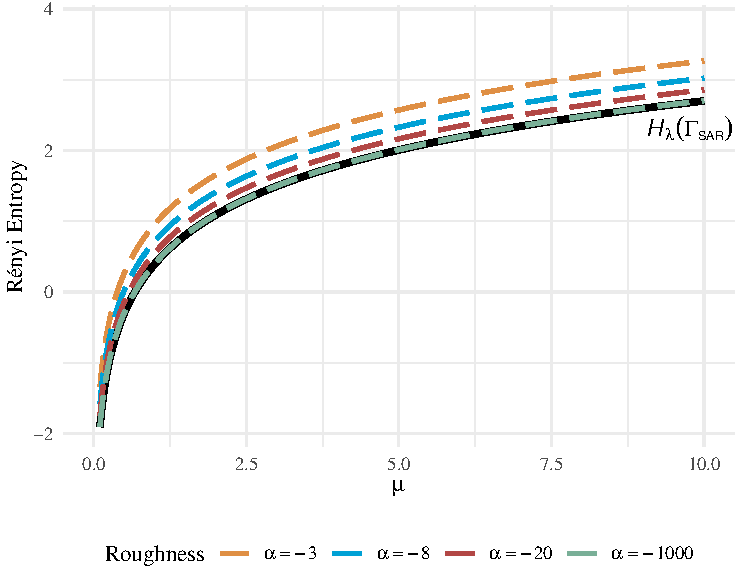
\includegraphics[width=0.45\textwidth,height=\textheight]{R0-Renyi-entropy-sar_files/figure-pdf/fig-plot-1.pdf}
%DIFDELCMD < 

%DIFDELCMD < }
%DIFDELCMD < 

%DIFDELCMD < %%%
\DIFdelendFL \DIFaddbeginFL \centering
  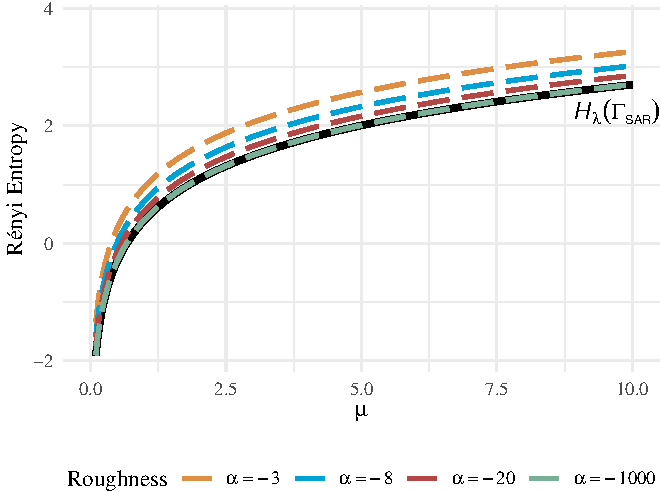
\includegraphics[width=0.42\textwidth]{Figures-R1/fig-convergence-1.pdf}
  \vspace{0.5em}
  \DIFaddendFL \caption{\DIFdelbeginFL %DIFDELCMD < \label{fig-plot}%%%
\DIFdelFL{\(H_{\lambda}(\mathcal{G}^0_I)\) converges }\DIFdelendFL \DIFaddbeginFL \DIFaddFL{Convergence of $H_{\lambda}(\mathcal{G}^0_I)$ }\DIFaddendFL to \DIFdelbeginFL \DIFdelFL{the \(H_{\lambda}(\Gamma_{\text{SAR}})\) when \(\alpha\to-\infty\), with
\(L=8\) and \(\lambda=0.8\)}\DIFdelendFL \DIFaddbeginFL \DIFaddFL{$H_{\lambda}(\Gamma_{\text{SAR}})$ as $\alpha$ decreases}\DIFaddendFL .}
  \DIFdelbeginFL %DIFDELCMD < 

%DIFDELCMD < %%%
\DIFdelendFL \DIFaddbeginFL \label{fig-convergence}
\DIFaddendFL \end{figure}
%DIF < 

\subsection{Non-parametric Estimation of Rényi
Entropy}\label{non-parametric-estimation-of-ruxe9nyi-entropy}

In order to estimate~\eqref{E:entropy2} from a random sample, one may
estimate the parameters that index the probability density function
\(f\) and integrate\DIFdelbegin \DIFdel{. This approach relies heavily }\DIFdelend \DIFaddbegin \DIFadd{, an approach that relies }\DIFaddend on the model assumptions\DIFdelbegin \DIFdel{and the absence of outliers.
Alternatively, one may estimate
directly \(f\). Such non-parametric estimation of \(H(Z)\) has been
widely studied using spacing-based estimators, which rely on differences
between order
statistics~\mbox{%DIFAUXCMD
\citeproc{ref-vasicek1976test}{{[}17{]}}}\hskip0pt%DIFAUXCMD
--\mbox{%DIFAUXCMD
\citeproc{ref-IbrahimAlOmari2014}{{[}21{]}}}\hskip0pt%DIFAUXCMD
.
}\DIFdelend \DIFaddbegin \DIFadd{.
}\DIFaddend Recently, Al-Labadi et al.~\DIFdelbegin \DIFdel{\mbox{%DIFAUXCMD
\citeproc{ref-AlLabadi2024}{{[}22{]}}
}\hskip0pt%DIFAUXCMD
}\DIFdelend \DIFaddbegin \DIFadd{\mbox{%DIFAUXCMD
\citeproc{ref-AlLabadi2024}{{[}13{]}}
}\hskip0pt%DIFAUXCMD
}\DIFaddend proposed a non-parametric estimator for Rényi entropy \DIFdelbegin \DIFdel{following this
approach}\DIFdelend \DIFaddbegin \DIFadd{based on
non-parametric estimation using differences between order statistics
(spacings)}\DIFaddend .

Let \(\bm{Z}=(Z_1, Z_2,\ldots,Z_n)\) be an independent and identically
distributed random sample of size \(n\) from \DIFdelbegin \DIFdel{a distribution \(F\)}\DIFdelend \DIFaddbegin \DIFadd{\(Z \sim F\)}\DIFaddend , and let
\(Z_{(1)} \leq Z_{(2)} \leq \dots \leq Z_{(n)}\) denote its order
statistics. The \(m\)-spacing density estimator is defined as: \[
f_n(Z_{(i)}) = \frac{c_i m / n}{Z_{(i+m)} - Z_{(i-m)}},
\] where \(Z_{(i-m)} = Z_{(1)}\) when \(i \leq m\), and
\(Z_{(i+m)} = Z_{(n)}\) if \(i \geq n - m\). The coefficient \(c_i\) is
given by: \[
c_i = 
\begin{cases}
\frac{m + i - 1}{m}, & \text{if } 1 \leq i \leq m, \\%[6pt]
2, & \text{if } m+1 \leq i \leq n - m, \\%[6pt]
\frac{n + m - i}{m}, & \text{if } n - m + 1 \leq i \leq n.
\end{cases}
\] \DIFdelbegin %DIFDELCMD < 

%DIFDELCMD < %%%
\DIFdel{Following Vasicek~\mbox{%DIFAUXCMD
\citeproc{ref-vasicek1976test}{{[}17{]}} }\hskip0pt%DIFAUXCMD
and Ebrahimi
et al.~\mbox{%DIFAUXCMD
\citeproc{ref-Ebrahimi1994}{{[}19{]}} }\hskip0pt%DIFAUXCMD
for Shannon entropy
estimation, and using the \(m\)-spacing density estimator, the }\DIFdelend \DIFaddbegin \DIFadd{The }\DIFaddend Rényi entropy can be estimated \DIFdelbegin \DIFdel{as: }\DIFdelend \DIFaddbegin \DIFadd{with this density estimator as
}\DIFaddend \begin{align}
\label{eq:est_R}
\widehat{H}_\lambda(\bm{Z}) = \frac{1}{1 - \lambda} \ln \left[\frac{1}{n} \sum_{i=1}^{n} \left( \frac{c_i m / n}{Z_{(i+m)} - Z_{(i-m)}} \right)^{\lambda - 1} \right].
\end{align} This estimator is asymptotically consistent, i.e., it
converges in probability to the true value when \(m,n\rightarrow\infty\)
and \(m/n\rightarrow0\). We \DIFdelbegin \DIFdel{used }\DIFdelend \DIFaddbegin \DIFadd{use }\DIFaddend the heuristic spacing
\(m=\left[\sqrt{n}+0.5\right]\).

\section{PROPOSED METHODOLOGY}\label{sec:met}

\subsection{\DIFdelbegin %DIFDELCMD < \texorpdfstring{On \(\lambda\) optimality for a sample
%DIFDELCMD < size}{On \textbackslash lambda optimality for a sample size}%%%
\DIFdelend \DIFaddbegin \texorpdfstring{Finding an optimal value of
\(\lambda\)}{Finding an optimal value of \textbackslash lambda}\DIFaddend }\DIFdelbegin %DIFDELCMD < \label{on-lambda-optimality-for-a-sample-size}
%DIFDELCMD < %%%
\DIFdelend \DIFaddbegin \label{finding-an-optimal-value-of-lambda}
\DIFaddend 

We aim to determine the optimal order \(\lambda\) for the Rényi entropy
estimator \DIFdelbegin \DIFdel{for a sample size \(n=49\). To identify this optimal value, we
analyze both the }\DIFdelend \DIFaddbegin \DIFadd{using simulated samples of size \(n = 49\) from
\(Z\sim \Gamma_{\text{SAR}}(5,1)\). We computed the bias and the }\DIFaddend mean
squared error (MSE) \DIFdelbegin \DIFdel{and bias of the estimator
across different values of }\DIFdelend \DIFaddbegin \DIFadd{for varying }\DIFaddend \(\lambda\) \DIFdelbegin \DIFdel{. Lower MSE and bias indicate
better estimator performance in approximating the true entropy.
}%DIFDELCMD < 

%DIFDELCMD < %%%
\DIFdelend \DIFaddbegin \DIFadd{via a Monte Carlo
experiment. }\DIFaddend We found that \DIFdelbegin \DIFdel{the optimal value }\DIFdelend for \(L > 1\)\DIFdelbegin \DIFdel{is \(\lambda = 0.9\), as
it minimizes the
}\DIFdelend \DIFaddbegin \DIFadd{, \(\lambda = 0.9\) yields the
lowest }\DIFaddend MSE while maintaining a low bias\DIFaddbegin \DIFadd{, thus offering a favorable
trade-off between bias and variance. As shown in
Fig.~\ref{fig-optimal_order},~\(\lambda = 0.85\) produces slightly lower
bias, but results in higher MSE, supporting the choice of
\(\lambda = 0.9\)}\DIFaddend .
\DIFdelbegin \DIFdel{However,}\DIFdelend \DIFaddbegin 

\begin{figure}[hbt]
  \centering
  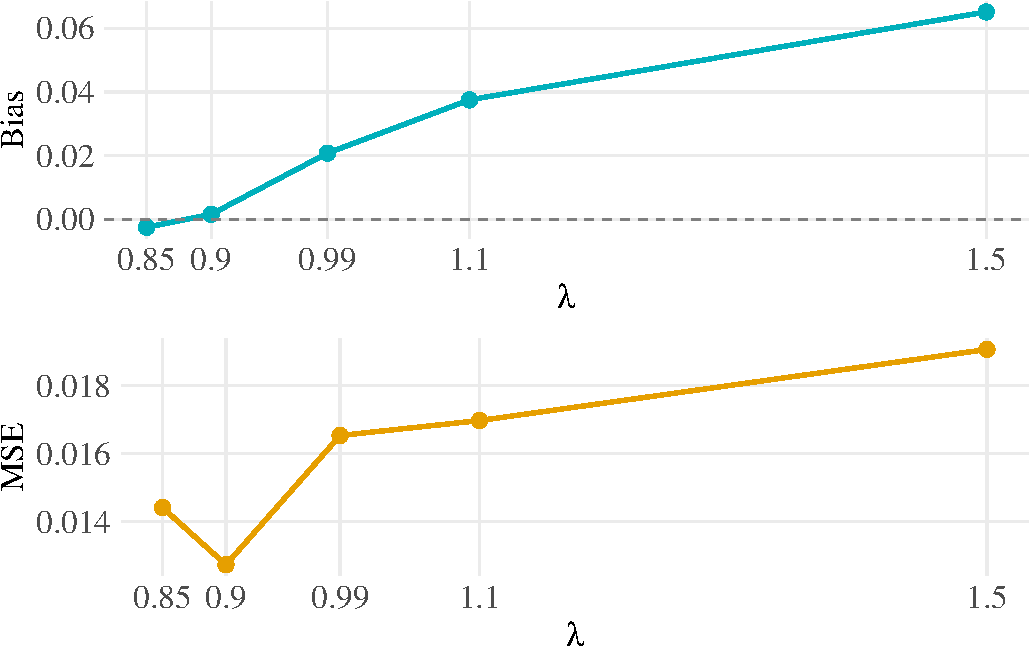
\includegraphics[width=0.42\textwidth]{Figures-R1/fig-optimal_order-1.pdf}
  \vspace{0.5em}
  \caption{\DIFaddFL{Bias and MSE as a function of $\lambda$, with $n=49$, $L=5$.}}
  \label{fig-optimal_order}
\end{figure}

\DIFadd{Particularly, }\DIFaddend for \(L = 1\), the optimal \(\lambda\) tends to be higher,
and we \DIFdelbegin \DIFdel{chose
}\DIFdelend \DIFaddbegin \DIFadd{choose }\DIFaddend \(\lambda = 3\) to achieve good results.
\DIFdelbegin \DIFdel{Fig.~\ref{fig-plotf}
illustrates the case for \(L = 5\).
}\DIFdelend 

\DIFdelbegin %DIFDELCMD < \begin{figure}[hbt]
%DIFDELCMD < 

%DIFDELCMD < \centering{
%DIFDELCMD < 

%DIFDELCMD < \includegraphics[width=0.42\textwidth,height=\textheight]{R0-Renyi-entropy-sar_files/figure-pdf/fig-plotf-1.pdf}
%DIFDELCMD < 

%DIFDELCMD < }
%DIFDELCMD < 

%DIFDELCMD < %%%
%DIFDELCMD < \caption{%
{%DIFAUXCMD
%DIFDELCMD < \label{fig-plotf}%%%
\DIFdelFL{Bias and MSE as a function of \(\lambda\),
with \(n=49\), \(L=5\).}}
%DIFAUXCMD
%DIFDELCMD < 

%DIFDELCMD < \end{figure}%%%
%DIF < 
%DIFDELCMD < 

%DIFDELCMD < %%%
\DIFdelend \subsection{Bootstrap Correction for Entropy
Estimator}\label{bootstrap-correction-for-entropy-estimator}

Following Refs.~\DIFdelbegin \DIFdel{\mbox{%DIFAUXCMD
\citeproc{ref-Frery2024}{{[}13{]}}}\hskip0pt%DIFAUXCMD
,
\mbox{%DIFAUXCMD
\citeproc{ref-Alpala2024}{{[}23{]}}}\hskip0pt%DIFAUXCMD
, we refined }\DIFdelend \DIFaddbegin \DIFadd{\mbox{%DIFAUXCMD
\citeproc{ref-Frery2024}{{[}11{]}}}\hskip0pt%DIFAUXCMD
,
\mbox{%DIFAUXCMD
\citeproc{ref-Alpala2024}{{[}14{]}}}\hskip0pt%DIFAUXCMD
, we refine }\DIFaddend the non-parametric
entropy estimator \(\widehat{H}_{\lambda}\) in~\eqref{eq:est_R} \DIFdelbegin \DIFdel{reducing
its bias }\DIFdelend with
bootstrap, obtaining \(\widetilde{H}_{\lambda}\): \DIFdelbegin \[
\DIFdel{\widetilde{H}_{\lambda} = 2\widehat{H}_{\lambda}(\bm{Z}) - \frac{1}{B} \sum_{b=1}^{B} \widehat{H}_{\lambda}(\bm{Z}^{(b)}),
}\]%DIFAUXCMD
\DIFdelend \DIFaddbegin \begin{equation*}
\DIFadd{\widetilde{H}_{\lambda} = 2\widehat{H}_{\lambda}(\bm{Z}) - \frac{1}{B} \sum_{b=1}^{B} \widehat{H}_{\lambda}(\bm{Z}^{(b)}),
}\end{equation*}\DIFaddend  where \(B\) is the number of bootstrap replications, and
\(\bm{Z}^{(b)}\) \DIFdelbegin \DIFdel{is }\DIFdelend \DIFaddbegin \DIFadd{denotes }\DIFaddend the \(b\)-th resampled dataset obtained by
drawing \(n\) observations with replacement from \(\bm{Z}\).

A Monte Carlo study with \(1000\) replications for each sample size
\(n \in \{9, 25, 49, 81, 121\}\) from the \(\Gamma_{\text{SAR}}\) (\DIFdelbegin \DIFdel{\(\mu=1, L=5\)}\DIFdelend \DIFaddbegin \DIFadd{5,1}\DIFaddend )
confirms that for \(\lambda=0.9\), the bootstrap-corrected estimator
\(\widetilde{H}_{\lambda}\) (\(B=200\)) reduces both bias and MSE
compared to the original \(\widehat{H}_{\lambda}\), with significant
improvements for small sample sizes, as shown in
\DIFdelbegin \DIFdel{~}\DIFdelend Fig.~\DIFdelbegin \DIFdel{\ref{fig-Plot_bias_msef3}}\DIFdelend \DIFaddbegin \DIFadd{\ref{fig-bias_mse}}\DIFaddend .

\begin{figure}[hbt]
  \DIFdelbeginFL %DIFDELCMD < 

%DIFDELCMD < \centering{
%DIFDELCMD < 

%DIFDELCMD < \includegraphics[width=0.42\textwidth,height=\textheight]{R0-Renyi-entropy-sar_files/figure-pdf/fig-Plot_bias_msef3-1.pdf}
%DIFDELCMD < 

%DIFDELCMD < }
%DIFDELCMD < 

%DIFDELCMD < %%%
\DIFdelendFL \DIFaddbeginFL \centering
  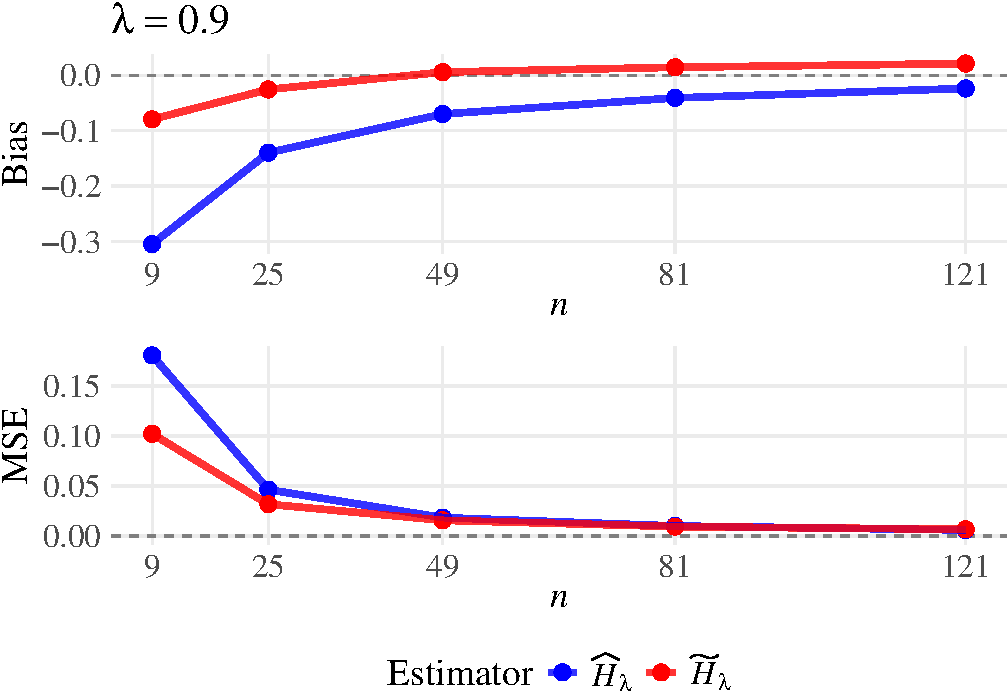
\includegraphics[width=0.40\textwidth]{Figures-R1/fig-bias_mse-1.pdf}
  \vspace{0.1em}
  \DIFaddendFL \caption{\DIFdelbeginFL %DIFDELCMD < \label{fig-Plot_bias_msef3}%%%
\DIFdelendFL Bias and MSE of the Rényi entropy estimators for \DIFdelbeginFL \DIFdelFL{\(\Gamma_{\text{SAR}}\)}\DIFdelendFL \DIFaddbeginFL \DIFaddFL{$\Gamma_{\text{SAR}}$}\DIFaddendFL .}
  \DIFdelbeginFL %DIFDELCMD < 

%DIFDELCMD < %%%
\DIFdelendFL \DIFaddbeginFL \label{fig-bias_mse}
\DIFaddendFL \end{figure}
%DIF < 

\DIFdelbegin \DIFdel{We use the \(\widetilde{H}_{\lambda}\) estimator for subsequent
simulations.
}%DIFDELCMD < 

%DIFDELCMD < %%%
\DIFdelend \subsection{Hypothesis Testing}\label{hypothesis-testing}

We test whether the observed data come from a homogeneous
(\(\Gamma_{\text{SAR}}\)) or a heterogeneous (\(\mathcal{G}^0_I\))
region, as follows: \begin{equation}\label{eq:hypothesis_test}
\begin{cases}
\mathcal{H}_0: \mathbb{E}[\widetilde{H}_{\lambda}] = H_{\lambda}(\Gamma_{\text{SAR}}) & \text{(Homogeneous region)}, \\[6pt]
\mathcal{H}_1: \mathbb{E}[\widetilde{H}_{\lambda}] = H_{\lambda}(\mathcal{G}^0_I) & \text{(Heterogeneous region)}.
\end{cases}
\end{equation}

Under \(\mathcal{H}_0\), the expected value of the entropy estimator
should match the theoretical \(H_{\lambda}(\Gamma_{\text{SAR}})\).
\DIFdelbegin \DIFdel{If
the estimated entropy significantly deviates from its expected value, we
reject \(\mathcal{H}_0\), indicating the presence of }\DIFdelend \DIFaddbegin \DIFadd{Significant deviations indicate }\DIFaddend heterogeneity.

\DIFdelbegin \DIFdel{Classical inference methods are inapplicable since homogeneity
corresponds to \(\alpha \to -\infty\) in the \(\mathcal{G}^0_I\) model.
Instead, we }\DIFdelend \DIFaddbegin \subsection{\DIFadd{The Proposed Test}}\label{the-proposed-test}

\DIFadd{We }\DIFaddend propose a test statistic \DIFdelbegin \DIFdel{based on the Rényi entropy
estimator, comparing it with its theoretical expectation under
\(\mathcal{H}_0\) to distinguish between
homogeneous and heterogeneous
areas.
}%DIFDELCMD < 

%DIFDELCMD < %%%
\subsection{\DIFdel{The Proposed Test}}%DIFAUXCMD
\addtocounter{subsection}{-1}%DIFAUXCMD
%DIFDELCMD < \label{the-proposed-test}
%DIFDELCMD < 

%DIFDELCMD < %%%
\DIFdel{Assume we have an estimator \(\widetilde{H}_{\lambda}\) for the Rényi
entropy of an arbitrary model. For testing~\eqref{eq:hypothesis_test},
this estimator is expected to be close to the theoretical expression
given in Equation~\eqref{eq-HGammaSAR}. }\DIFdelend \DIFaddbegin \DIFadd{that identifies the discrepancy between
estimated and theoretical entropy under homogeneity. }\DIFaddend Since \(L\geq1\) is
known, we define the test statistic as follows: \begin{multline}
\label{eq-test}
S_{\widetilde{H}_{\lambda}}(\bm{Z}; L) = \widetilde{H}_{\lambda} - \bigl\{\ln \widehat{\mu} - \ln L + \frac{1}{1-\lambda}
\bigl[-\lambda\,\ln\Gamma(L) \\ 
+ \ln\Gamma\bigl(\lambda(L-1)+1\bigr)  
- \bigl(\lambda(L-1)+1\bigr)\,\ln\lambda
\bigr]\bigr\},
\end{multline} where \(\widehat{\mu}={n}^{-1}\sum_{i=1}^n Z_{i}\) is the
sample mean. \DIFdelbegin \DIFdel{This test statistic should be }\DIFdelend \DIFaddbegin \DIFadd{The test statistic can be interpreted as: }\[
\DIFadd{S_{\widetilde H_\lambda} 
= 
\underbrace{\widetilde H_\lambda}_{\text{estimated}} 
\;-\;
\underbrace{H_\lambda\bigl(\Gamma_{\mathrm{SAR}}\bigr)}_{\text{theoretical under } H_0}\hspace{-0.5em},
}\] \DIFadd{the difference between the estimated entropy and the expected value
under homogeneity. Values }\DIFaddend close to zero \DIFdelbegin \DIFdel{when the null
hypothesis holds. }\DIFdelend \DIFaddbegin \DIFadd{indicate that the region behaves
like fully developed speckle, while large positive values signal excess
entropy and, thus, heterogeneity. This formulation avoids the need to
estimate \(\mathcal{G}^0_I\) parameters such as \(\alpha\), offering a
simple, interpretable, and statistically grounded test. Moreover, the
method remains effective for small samples, aided by the bootstrap bias
correction.
}

\DIFaddend Fig.~\DIFdelbegin \DIFdel{\ref{fig-density_entropyR} }\DIFdelend \DIFaddbegin \DIFadd{\ref{fig-densities} }\DIFaddend shows the empirical \DIFdelbegin \DIFdel{density of
\(S_{\widetilde{H}_{\lambda}}(\bm{Z}; L)\), based on }\DIFdelend \DIFaddbegin \DIFadd{distribution of
\(S_{\widetilde{H}_{\lambda}}\) under \(\mathcal{H}_0\), obtained from
}\DIFaddend \(10^4\) \DIFdelbegin \DIFdel{replications of the \(\Gamma_{\text{SAR}}\) model for each sample size
\(n \in \{49,81, 121\}\) with }\DIFdelend \DIFaddbegin \DIFadd{Monte Carlo experiments with varying sample sizes
(\(n \in {49,81,121}\)), }\DIFaddend \(\lambda=0.9\)\DIFdelbegin \DIFdel{and \(L \in \{5,18\}\). }\DIFdelend \DIFaddbegin \DIFadd{, and \(L \in {5,18}\). The
concentration around zero confirms the expected behavior of the test,
while the heavy tails indicate sensitivity to deviations, enabling the
detection of subtle texture changes.
}\DIFaddend 

\begin{figure}[hbt]
  \DIFdelbeginFL %DIFDELCMD < 

%DIFDELCMD < \centering{
%DIFDELCMD < 

%DIFDELCMD < \includegraphics[width=0.47\textwidth,height=\textheight]{R0-Renyi-entropy-sar_files/figure-pdf/fig-density_entropyR-1.pdf}
%DIFDELCMD < 

%DIFDELCMD < }
%DIFDELCMD < 

%DIFDELCMD < %%%
\DIFdelendFL \DIFaddbeginFL \centering
  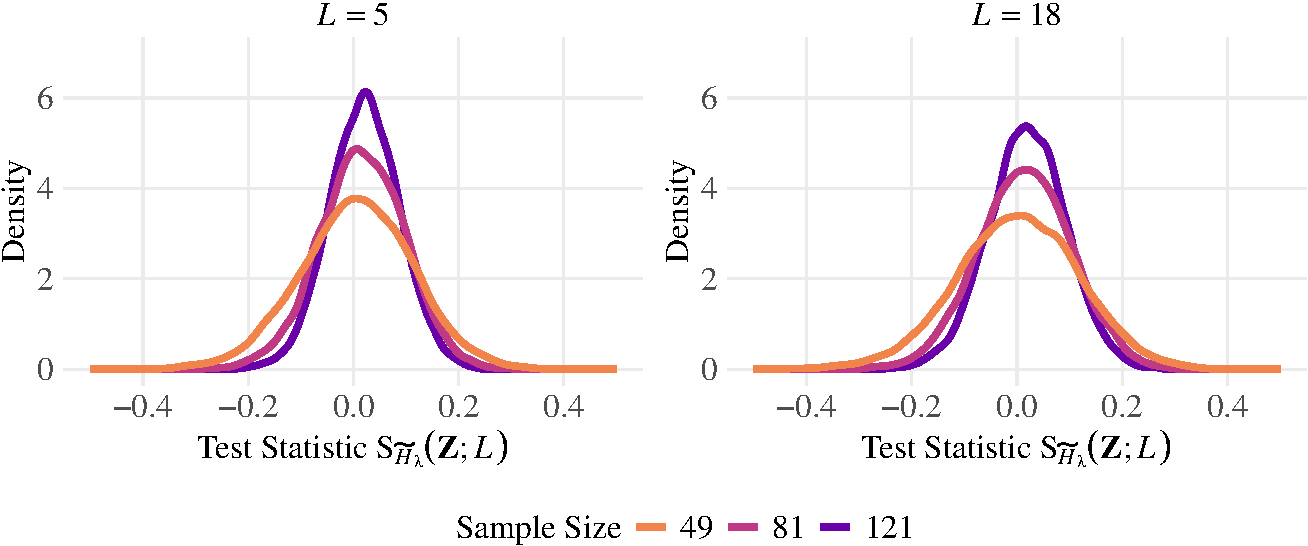
\includegraphics[width=0.42\textwidth]{Figures-R1/fig-densities-1.pdf}
  \vspace{0.2em}
  \DIFaddendFL \caption{\DIFdelbeginFL %DIFDELCMD < \label{fig-density_entropyR}%%%
\DIFdelendFL Empirical densities of \DIFdelbeginFL \DIFdelFL{\(S_{\widetilde{H}_{\lambda}}(\bm{Z}; L)\) }\DIFdelendFL \DIFaddbeginFL \DIFaddFL{$S_{\widetilde{H}_{\lambda}}(\bm{Z}; L)$ }\DIFaddendFL under \DIFdelbeginFL \DIFdelFL{\(\mathcal{H}_0\)}\DIFdelendFL \DIFaddbeginFL \DIFaddFL{$\mathcal{H}_0$}\DIFaddendFL .}
  \DIFdelbeginFL %DIFDELCMD < 

%DIFDELCMD < %%%
\DIFdelendFL \DIFaddbeginFL \label{fig-densities}
\DIFaddendFL \end{figure}
%DIF < 

Vasicek~\DIFdelbegin \DIFdel{\mbox{%DIFAUXCMD
\citeproc{ref-vasicek1976test}{{[}17{]}} }\hskip0pt%DIFAUXCMD
}\DIFdelend \DIFaddbegin \DIFadd{\mbox{%DIFAUXCMD
\citeproc{ref-vasicek1976test}{{[}15{]}} }\hskip0pt%DIFAUXCMD
}\DIFaddend proved that, for
sufficiently large samples, \(S_{\widetilde{H}_{\lambda}}(\bm{Z}; L)\)
asymptotically follows a normal distribution: \begin{equation*}
S_{\widetilde{H}_{\lambda}}(\bm{Z}; L) 
\DIFdelbegin %DIFDELCMD < \overset{d}{\longrightarrow} %%%
\DIFdelend \DIFaddbegin \overset{\mathcal{D}}{\underset{n \to \infty}{\longrightarrow}} 
\DIFaddend \mathcal{N}(\mu_S,\,\sigma^{2}_S)\DIFdelbegin \DIFdel{\,}\DIFdelend ,
\end{equation*} where \DIFdelbegin \DIFdel{\(d\) }\DIFdelend \DIFaddbegin \DIFadd{\(\mathcal{D}\) }\DIFaddend represents convergence in
distribution. Here,
\(\mu_S  = \mathbb{E}[S_{\widetilde{H}_{\lambda}}(\bm{Z}; L)]\) and
\(\sigma^{2}_S = \text{Var}[S_{\widetilde{H}_{\lambda}}(\bm{Z}; L)]\)
are the theoretical mean and variance of
\(S_{\widetilde{H}_{\lambda}}(\bm{Z}; L)\).

The standardized test statistic
\DIFdelbegin \DIFdel{\(\varepsilon = ({S_{\widetilde{H}_{\lambda}}(\bm{Z}; L) - \hat{\mu}_S})/{\hat{\sigma}_S}\)
}\DIFdelend \DIFaddbegin \DIFadd{\(\varepsilon = ({S_{\widetilde{H}_{\lambda}}(\bm{Z}; L) - \widehat{\mu}_S})/{\widehat{\sigma}_S}\)
}\DIFaddend is asymptotically standard normal distributed, where \DIFdelbegin \DIFdel{\(\hat{\mu}_S\) and \(\hat{\sigma}_S\) are the empirical }\DIFdelend \DIFaddbegin \DIFadd{\(\widehat{\mu}_S\)
and \(\widehat{\sigma}_S\) are the estimated }\DIFaddend mean and standard deviation
of \(S_{\widetilde{H}_{\lambda}}(\bm{Z}; L)\), obtained by Monte Carlo
simulations under the null hypothesis. Thus, \DIFaddbegin \DIFadd{we compute }\DIFaddend the \(p\)-values
\DIFdelbegin \DIFdel{are
calculated }\DIFdelend as \(2\Phi(-|\varepsilon|)\), where \(\Phi(\cdot)\) is the cumulative
distribution function of the standard normal \DIFdelbegin \DIFdel{distribution.
Fig.~\ref{fig-density_entropyR_standardized0} shows smoothed histograms
of standardized test statistics.
}\DIFdelend \DIFaddbegin \DIFadd{law.
}\DIFaddend 

\DIFdelbegin %DIFDELCMD < \begin{figure}[hbt]
%DIFDELCMD < 

%DIFDELCMD < \centering{
%DIFDELCMD < 

%DIFDELCMD < 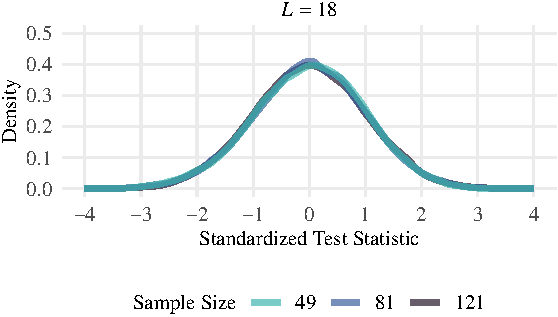
\includegraphics[width=0.35\textwidth,height=\textheight]{R0-Renyi-entropy-sar_files/figure-pdf/fig-density_entropyR_standardized0-1.pdf}
%DIFDELCMD < 

%DIFDELCMD < }
%DIFDELCMD < 

%DIFDELCMD < %%%
%DIFDELCMD < \caption{%
{%DIFAUXCMD
%DIFDELCMD < \label{fig-density_entropyR_standardized0}%%%
\DIFdelFL{Standardized
empirical densities of \(S_{\widetilde{H}_{\lambda}}(\bm{Z}; L)\) under
\(\mathcal{H}_0\).}}
%DIFAUXCMD
%DIFDELCMD < 

%DIFDELCMD < \end{figure}%%%
%DIF < 
%DIFDELCMD < 

%DIFDELCMD < %%%
\DIFdelend In general, \DIFdelbegin \DIFdel{hypotheses }\DIFdelend \DIFaddbegin \DIFadd{hypothesis }\DIFaddend tests aim to control the Type~I error rate (size)
with high test power (sensitivity to departures from \(\mathcal{H}_0\),
low Type~II error rate). To assess these properties, we performed a
Monte Carlo simulation with \(1000\) replications at significance levels
\SI{1}{\percent}, \SI{5}{\percent}, and \SI{10}{\percent}, evaluating
the test under the null hypothesis (\(\Gamma_{\text{SAR}}\)
distribution), varying sample size and values of \(L\) for \(\mu=1\).
The observed Type~I error rates align with the nominal values,
confirming the test validity.

Further, we examined the power under the alternative hypothesis
(\(\mathcal{G}^0_I\) distribution) with \(\mu=1\), \(\lambda=0.9\) and
\(\alpha=-2\). As expected, power improves as the sample size and the
number of looks increase, demonstrating the test effectiveness. The
results are shown in Table~\ref{tab:table_size_power}.

\begin{table}[htb]
\centering\centering
\caption{\label{tab:table_size_power}Size and Power of the $S_{\widetilde{H}_{\lambda}}(\bm{Z})$ test statistic.}
\resizebox{\ifdim\width>\linewidth\linewidth\else\width\fi}{!}{
\fontsize{7}{9}\selectfont
\begin{tabu} to \linewidth {>{\centering}X>{\centering}X>{\centering}X>{\centering}X>{\centering}X>{\centering}X>{\centering}X>{\centering}X}
\toprule
\multicolumn{2}{c}{ } & \multicolumn{3}{c}{Size} & \multicolumn{3}{c}{Power} \\
\cmidrule(l{3pt}r{3pt}){3-5} \cmidrule(l{3pt}r{3pt}){6-8}
\multicolumn{1}{c}{$\bm{L}$} & \multicolumn{1}{c}{$\bm{n}$} & \multicolumn{1}{c}{$\hphantom{00}\SI{1}{\percent}$} & \multicolumn{1}{c}{$\hphantom{00}\SI{5}{\percent}$} & \multicolumn{1}{c}{$\hphantom{00}\SI{10}{\percent}$} & \multicolumn{1}{c}{$\hphantom{00}\SI{1}{\percent}$} & \multicolumn{1}{c}{$\hphantom{00}\SI{5}{\percent}$} & \multicolumn{1}{c}{$\hphantom{00}\SI{10}{\percent}$}\\
\midrule
 & 25 & $\phantom{-}0.014$ & $\phantom{-}0.050$ & $\phantom{-}0.100$ & $\phantom{-}0.978$ & $\phantom{-}0.994$ & $\phantom{-}0.993$\\

 & 49 & $\phantom{-}0.011$ & $\phantom{-}0.048$ & $\phantom{-}0.109$ & $\phantom{-}0.994$ & $\phantom{-}1.000$ & $\phantom{-}0.999$\\

 & 81 & $\phantom{-}0.012$ & $\phantom{-}0.057$ & $\phantom{-}0.103$ & $\phantom{-}0.998$ & $\phantom{-}0.998$ & $\phantom{-}0.999$\\

\multirow{-4}{*}[1.5\dimexpr\aboverulesep+\belowrulesep+\cmidrulewidth]{\centering\arraybackslash 5} & 121 & $\phantom{-}0.013$ & $\phantom{-}0.061$ & $\phantom{-}0.116$ & $\phantom{-}0.999$ & $\phantom{-}0.999$ & $\phantom{-}0.997$\\
\cmidrule{1-8}
 & 25 & $\phantom{-}0.010$ & $\phantom{-}0.051$ & $\phantom{-}0.105$ & $\phantom{-}0.996$ & $\phantom{-}0.999$ & $\phantom{-}1.000$\\

 & 49 & $\phantom{-}0.008$ & $\phantom{-}0.056$ & $\phantom{-}0.109$ & $\phantom{-}1.000$ & $\phantom{-}0.999$ & $\phantom{-}1.000$\\

 & 81 & $\phantom{-}0.012$ & $\phantom{-}0.052$ & $\phantom{-}0.097$ & $\phantom{-}0.999$ & $\phantom{-}0.999$ & $\phantom{-}0.999$\\

\multirow{-4}{*}[1.5\dimexpr\aboverulesep+\belowrulesep+\cmidrulewidth]{\centering\arraybackslash 8} & 121 & $\phantom{-}0.016$ & $\phantom{-}0.070$ & $\phantom{-}0.116$ & $\phantom{-}0.998$ & $\phantom{-}1.000$ & $\phantom{-}0.999$\\
\cmidrule{1-8}
 & 25 & $\phantom{-}0.016$ & $\phantom{-}0.051$ & $\phantom{-}0.111$ & $\phantom{-}1.000$ & $\phantom{-}1.000$ & $\phantom{-}1.000$\\

 & 49 & $\phantom{-}0.014$ & $\phantom{-}0.047$ & $\phantom{-}0.098$ & $\phantom{-}1.000$ & $\phantom{-}1.000$ & $\phantom{-}1.000$\\

 & 81 & $\phantom{-}0.013$ & $\phantom{-}0.048$ & $\phantom{-}0.106$ & $\phantom{-}1.000$ & $\phantom{-}1.000$ & $\phantom{-}1.000$\\

\multirow{-4}{*}[1.5\dimexpr\aboverulesep+\belowrulesep+\cmidrulewidth]{\centering\arraybackslash 18} & 121 & $\phantom{-}0.012$ & $\phantom{-}0.066$ & $\phantom{-}0.110$ & $\phantom{-}1.000$ & $\phantom{-}1.000$ & $\phantom{-}1.000$\\
\bottomrule
\end{tabu}}
\end{table}

\DIFaddbegin \DIFadd{We applied the proposed test to SAR images using sliding windows of
\(7 \times 7\) pixels. For each window, we computed the test statistic
and calculated the \(p\)-value that quantifies the statistical evidence
against local homogeneity. High \(p\)-values, e.g., \(p > 0.05\),
indicate no evidence to reject homogeneity, while low values, e.g.,
\(p < 0.05\), suggest statistically significant deviations and are
interpreted as heterogeneity.
}

\DIFaddend \section{Applications to SAR Data}\label{sec:app}

\DIFdelbegin \DIFdel{In this section, we }\DIFdelend \DIFaddbegin \subsection{\DIFadd{Datasets}}\label{datasets}

\DIFadd{We }\DIFaddend compare two test statistics for detecting heterogeneity in SAR data:
(i) the Rényi entropy-based test,
\(S_{\widetilde{H}_{\lambda}}(\bm{Z}; L)\), described
in~\eqref{eq-test}; and (ii) the Shannon entropy-based test,
\(S_{\widetilde{H}_{\text{AO}}}(\bm{Z}; L)\), which is based on the
Al-Omari estimator proposed
in~\DIFdelbegin \DIFdel{\mbox{%DIFAUXCMD
\citeproc{ref-IbrahimAlOmari2014}{{[}21{]}} }\hskip0pt%DIFAUXCMD
}\DIFdelend \DIFaddbegin \DIFadd{\mbox{%DIFAUXCMD
\citeproc{ref-IbrahimAlOmari2014}{{[}16{]}} }\hskip0pt%DIFAUXCMD
}\DIFaddend and was improved via
bootstrap in our previous work. The details of this test can be found in
Frery et al.~\DIFdelbegin \DIFdel{\mbox{%DIFAUXCMD
\citeproc{ref-Frery2024}{{[}13{]}}}\hskip0pt%DIFAUXCMD
}\DIFdelend \DIFaddbegin \DIFadd{\mbox{%DIFAUXCMD
\citeproc{ref-Frery2024}{{[}11{]}}}\hskip0pt%DIFAUXCMD
}\DIFaddend .

\DIFdelbegin \DIFdel{We applied these tests to images covering urban, agricultural, and water
regions. We analyzed images from London , United Kingdom; the surroundings of Munich
, Germany; and Dublin Port, Ireland}\DIFdelend \DIFaddbegin \DIFadd{The selected scenes, acquired in HH polarization, correspond to the
surroundings of London (United Kingdom), the outskirts of Munich
(Germany), and the Dublin Port area (Ireland)}\DIFaddend , as shown in
Figs.~\DIFdelbegin \DIFdel{\ref{fig:london-a},~\ref{fig:munich-a}, and~\ref{fig:dublin-a}. All images were acquired in HH polarization.}\DIFdelend \DIFaddbegin \DIFadd{\ref{fig:london-sar}-\ref{fig:dublin-sar}. Corresponding optical
images (Figs.~\ref{fig:london-optical}--\ref{fig:dublin-optical})
illustrate land cover context. }\DIFaddend Table~\ref{tab:table_param} \DIFdelbegin \DIFdel{provides the
detailed acquisition parametersof these images.
}%DIFDELCMD < \renewcommand{\arraystretch}{3}
%DIFDELCMD < %%%
\DIFdelend \DIFaddbegin \DIFadd{details the
SAR acquisition parameters.
}\DIFaddend 

\DIFdelbegin %DIFDELCMD < \begin{table}[hbt]
%DIFDELCMD < %%%
\DIFdelendFL \DIFaddbeginFL \renewcommand{\arraystretch}{2.5}

\begin{table}[H]
\DIFaddendFL \centering\centering
\caption{\label{tab:table_param}Parameters of selected SAR images\DIFdelbeginFL \DIFdelFL{.}\DIFdelendFL }
\centering
\DIFdelbeginFL %DIFDELCMD < \resizebox{\ifdim\width>\linewidth\linewidth\else\width\fi}{!}{
%DIFDELCMD < \fontsize{21}{23}\selectfont
%DIFDELCMD < \begin{tabu} to \linewidth {>{\centering\arraybackslash}p{3.0cm}>{\centering\arraybackslash}p{3.7cm}>{\centering\arraybackslash}p{1.5cm}>{\centering\arraybackslash}p{4cm}>{\centering\arraybackslash}p{1.5cm}>{\centering\arraybackslash}p{4.0cm}>{\centering\arraybackslash}p{4.5cm}}
%DIFDELCMD < \toprule
%DIFDELCMD < \multicolumn{1}{c}{\textbf{Site}} & \multicolumn{1}{c}{\textbf{Mission}} & \multicolumn{1}{c}{\textbf{Band}} & \multicolumn{1}{c}{\textbf{Size (pixels)}} & \multicolumn{1}{c}{$\bm{L}$} & \multicolumn{1}{c}{\textbf{Resolution [m]}} & \multicolumn{1}{c}{\textbf{Acquisition Date}}\\
%DIFDELCMD < \midrule
%DIFDELCMD < London & TanDEM-X & X & $2000\times2000$ & $1$ & $0.99/0.99$ & 12-11-2021\\
%DIFDELCMD < Munich & UAVSAR & L & $1024\times1024$ & $12$ & $4.9/7.2$ & 16-04-2015\\
%DIFDELCMD < Dublin & TanDEM-X & X & $1100\times1100$ & $16$ & $1.35/1.35$ & 03-09-2017\\
%DIFDELCMD < \bottomrule
%DIFDELCMD < \end{tabu}}
%DIFDELCMD < %%%
\DIFdelendFL \DIFaddbeginFL \resizebox{\ifdim\width>\linewidth\linewidth\else\width\fi}{!}{
\fontsize{22}{24}\selectfont
\begin{tabu} to \linewidth {>{\centering\arraybackslash}p{3.0cm}>{\centering\arraybackslash}p{4.5cm}>{\centering\arraybackslash}p{1.5cm}>{\centering\arraybackslash}p{4cm}>{\centering\arraybackslash}p{1.5cm}>{\centering\arraybackslash}p{4.0cm}>{\centering\arraybackslash}p{4.5cm}}
\toprule
\multicolumn{1}{c}{\textbf{Scene}} & \multicolumn{1}{c}{\textbf{Mission}} & \multicolumn{1}{c}{\textbf{Band}} & \multicolumn{1}{c}{\textbf{Size (pixels)}} & \multicolumn{1}{c}{$\bm{L}$} & \multicolumn{1}{c}{\textbf{Resolution [m]}} & \multicolumn{1}{c}{\textbf{Acquisition Date}}\\
\midrule
London & TanDEM-X & X & $2000\times2000$ & $1$ & $0.99\times0.99$ & 12-11-2021\\
Munich & UAVSAR & L & $1024\times1024$ & $12$ & $4.9\times7.2$ & 16-04-2015\\
Dublin & TanDEM-X & X & $1100\times1100$ & $16$ & $1.35\times1.35$ & 03-09-2017\\
\bottomrule
\end{tabu}}
\DIFaddendFL \end{table}

\DIFdelbegin \DIFdel{We used sliding windows of size \(7\times 7\)}\DIFdelend \DIFaddbegin \DIFadd{For each SAR image, the number of looks \(L\) was obtained from the
product of azimuth and range looks provided in the metadata (SNAP). We
validated this nominal value with the equivalent number of looks (ENL)
from manually selected homogeneous areas using the classical formula
\(\text{ENL} = 1/\widehat{\text{CV}}^2\), based on the sample
coefficient of variation}\DIFaddend . The results \DIFdelbegin \DIFdel{are presented
as }\DIFdelend \DIFaddbegin \DIFadd{were consistent with the metadata.
We also verified that moderate deviations in \(L\) did not significantly
impact the outcome of the test, confirming the robustness of the
proposed method.
}

\subsection{\DIFadd{Qualitative Inspection}}\label{qualitative-inspection}

\DIFadd{The output consists of }\DIFaddend \(p\)-value maps and binary maps at a \(0.05\)
significance level. \DIFdelbegin \DIFdel{Figs.~\ref{fig:london-b}--\ref{fig:london-c},~\ref{fig:munich-b}--\ref{fig:munich-c},and~\ref{fig:dublin-b}--\ref{fig:dublin-c} correspond to
\(S_{\widetilde{H}_{\lambda}}(\bm{Z}; L)\),while
Figs.~\ref{fig:london-d}--\ref{fig:london-e},~\ref{fig:munich-d}--\ref{fig:munich-e},and~\ref{fig:dublin-d}--\ref{fig:dublin-e} correspond to
\(S_{\widetilde{H}_{\text{AO}}}(\bm{Z}; L)\).
}%DIFDELCMD < 

%DIFDELCMD < %%%
\DIFdelend The \(p\)-value \DIFdelbegin \DIFdel{maps use a color gradient}\DIFdelend \DIFaddbegin \DIFadd{maps use a color gradient
(Figs.~\ref{fig:london-renyi},~\ref{fig:london-shann},~\ref{fig:munich-renyi},~\ref{fig:munich-shann},~\ref{fig:dublin-renyi},~\ref{fig:dublin-shann})}\DIFaddend ,
where darker regions indicate areas with higher roughness, and lighter
regions denote \DIFdelbegin \DIFdel{smoother, }\DIFdelend less textured surfaces. The binary maps
\DIFdelbegin \DIFdel{classify these results: white areas
represent \(p\)-values greater than \(0.05\),indicating no statistical
evidence to reject the null hypothesis (homogeneous regions). In
contrast, black areas represent regions with \(p\)-values below
\(0.05\), providing statistical evidence to reject the null hypothesis
and indicating heterogeneity.
}%DIFDELCMD < 

%DIFDELCMD < %%%
\DIFdel{The }\DIFdelend \DIFaddbegin \DIFadd{(Figs.~\ref{fig:london-005-renyi},~\ref{fig:london-005-shann},~\ref{fig:munich-005-renyi},~\ref{fig:munich-005-shann},~\ref{fig:dublin-005-renyi},~\ref{fig:dublin-005-shann})
display heterogeneous detections in black (\(p<0.05\)) and homogeneous
areas in white (\(p \geq 0.05\)). Visually, the }\DIFaddend Rényi \DIFdelbegin \DIFdel{entropy-based test demonstrated }\DIFdelend \DIFaddbegin \DIFadd{test exhibits
}\DIFaddend greater sensitivity in detecting textural variations \DIFdelbegin \DIFdel{than the Shannon-based test }\DIFdelend due to the
flexibility provided by the parameter \(\lambda\)\DIFdelbegin \DIFdel{, as observed in the
binary maps in Figs.
~\ref{fig:london-c},~\ref{fig:munich-c},
and~\ref{fig:dublin-c}.
}\DIFdelend \DIFaddbegin \DIFadd{.
}\DIFaddend 

\begin{figure*}[hbt]
    \centering
    \DIFdelbeginFL %DIFDELCMD < \begin{subfigure}{0.17\textwidth}
%DIFDELCMD <         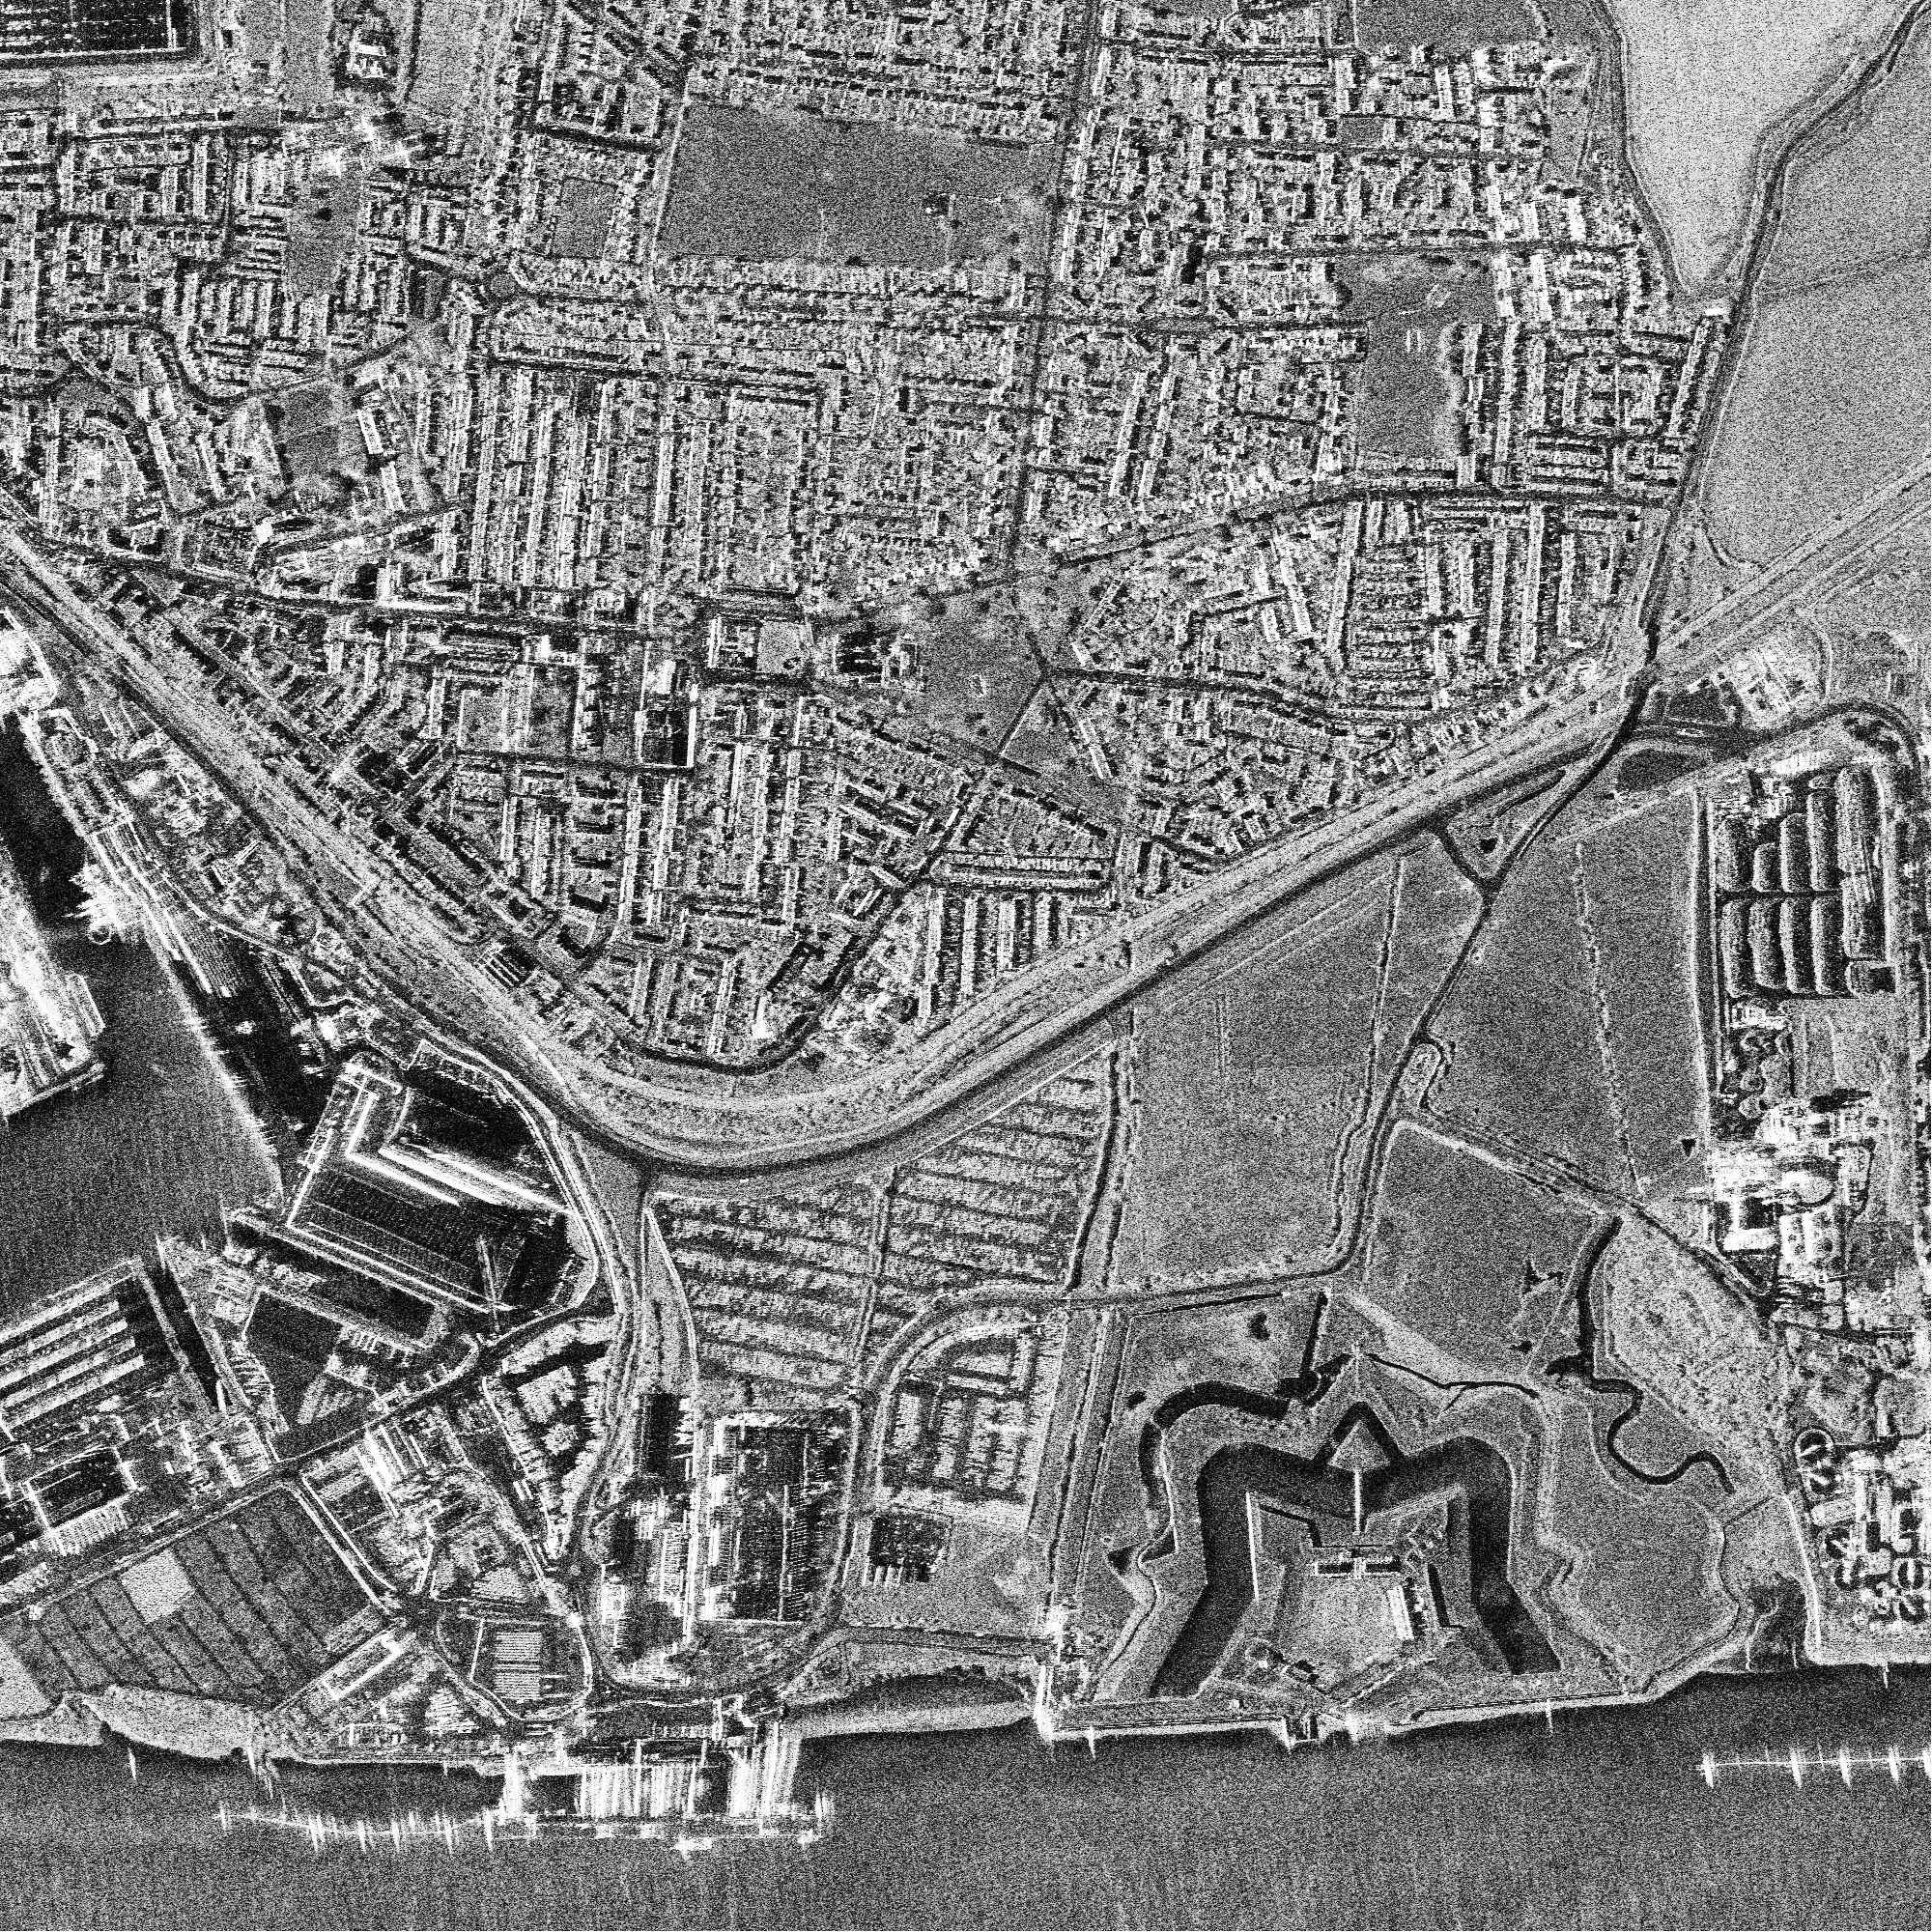
\includegraphics[width=\linewidth]{./Figures/london_2000.png}
%DIFDELCMD <         %%%
\DIFdelendFL \DIFaddbeginFL \begin{subfigure}{0.145\textwidth}
        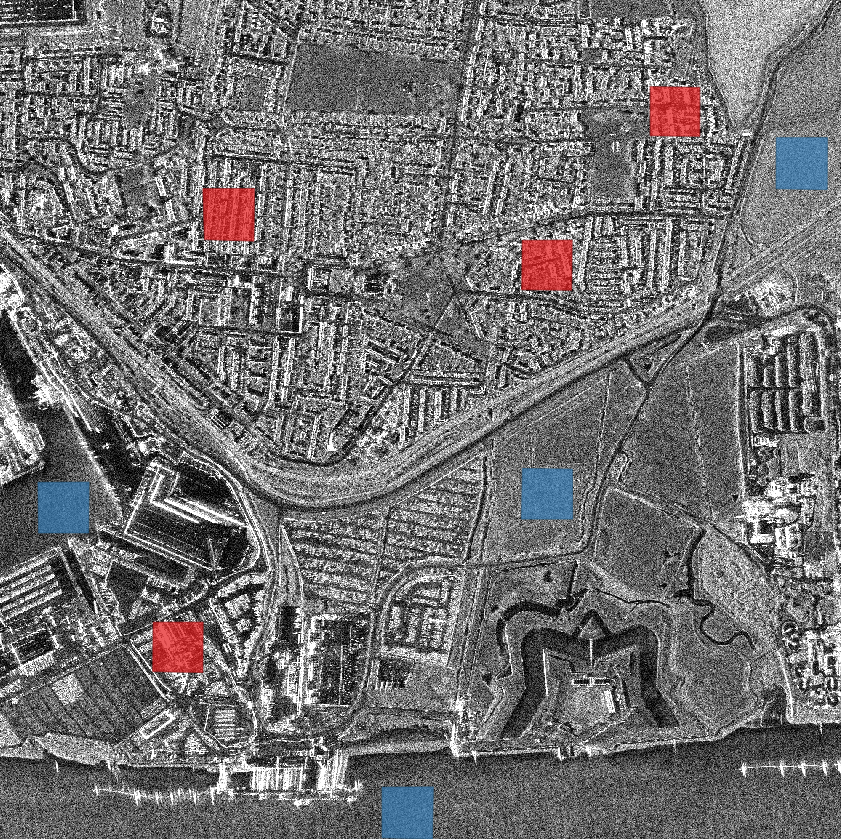
\includegraphics[width=\linewidth]{./Figures-R1/london_roi.png}
        \DIFaddendFL \caption{SAR image}
        \DIFdelbeginFL %DIFDELCMD < \label{fig:london-a}
%DIFDELCMD <     %%%
\DIFdelendFL \DIFaddbeginFL \label{fig:london-sar}
    \DIFaddendFL \end{subfigure}
    \DIFdelbeginFL %DIFDELCMD < \begin{subfigure}{0.22\textwidth}
%DIFDELCMD <         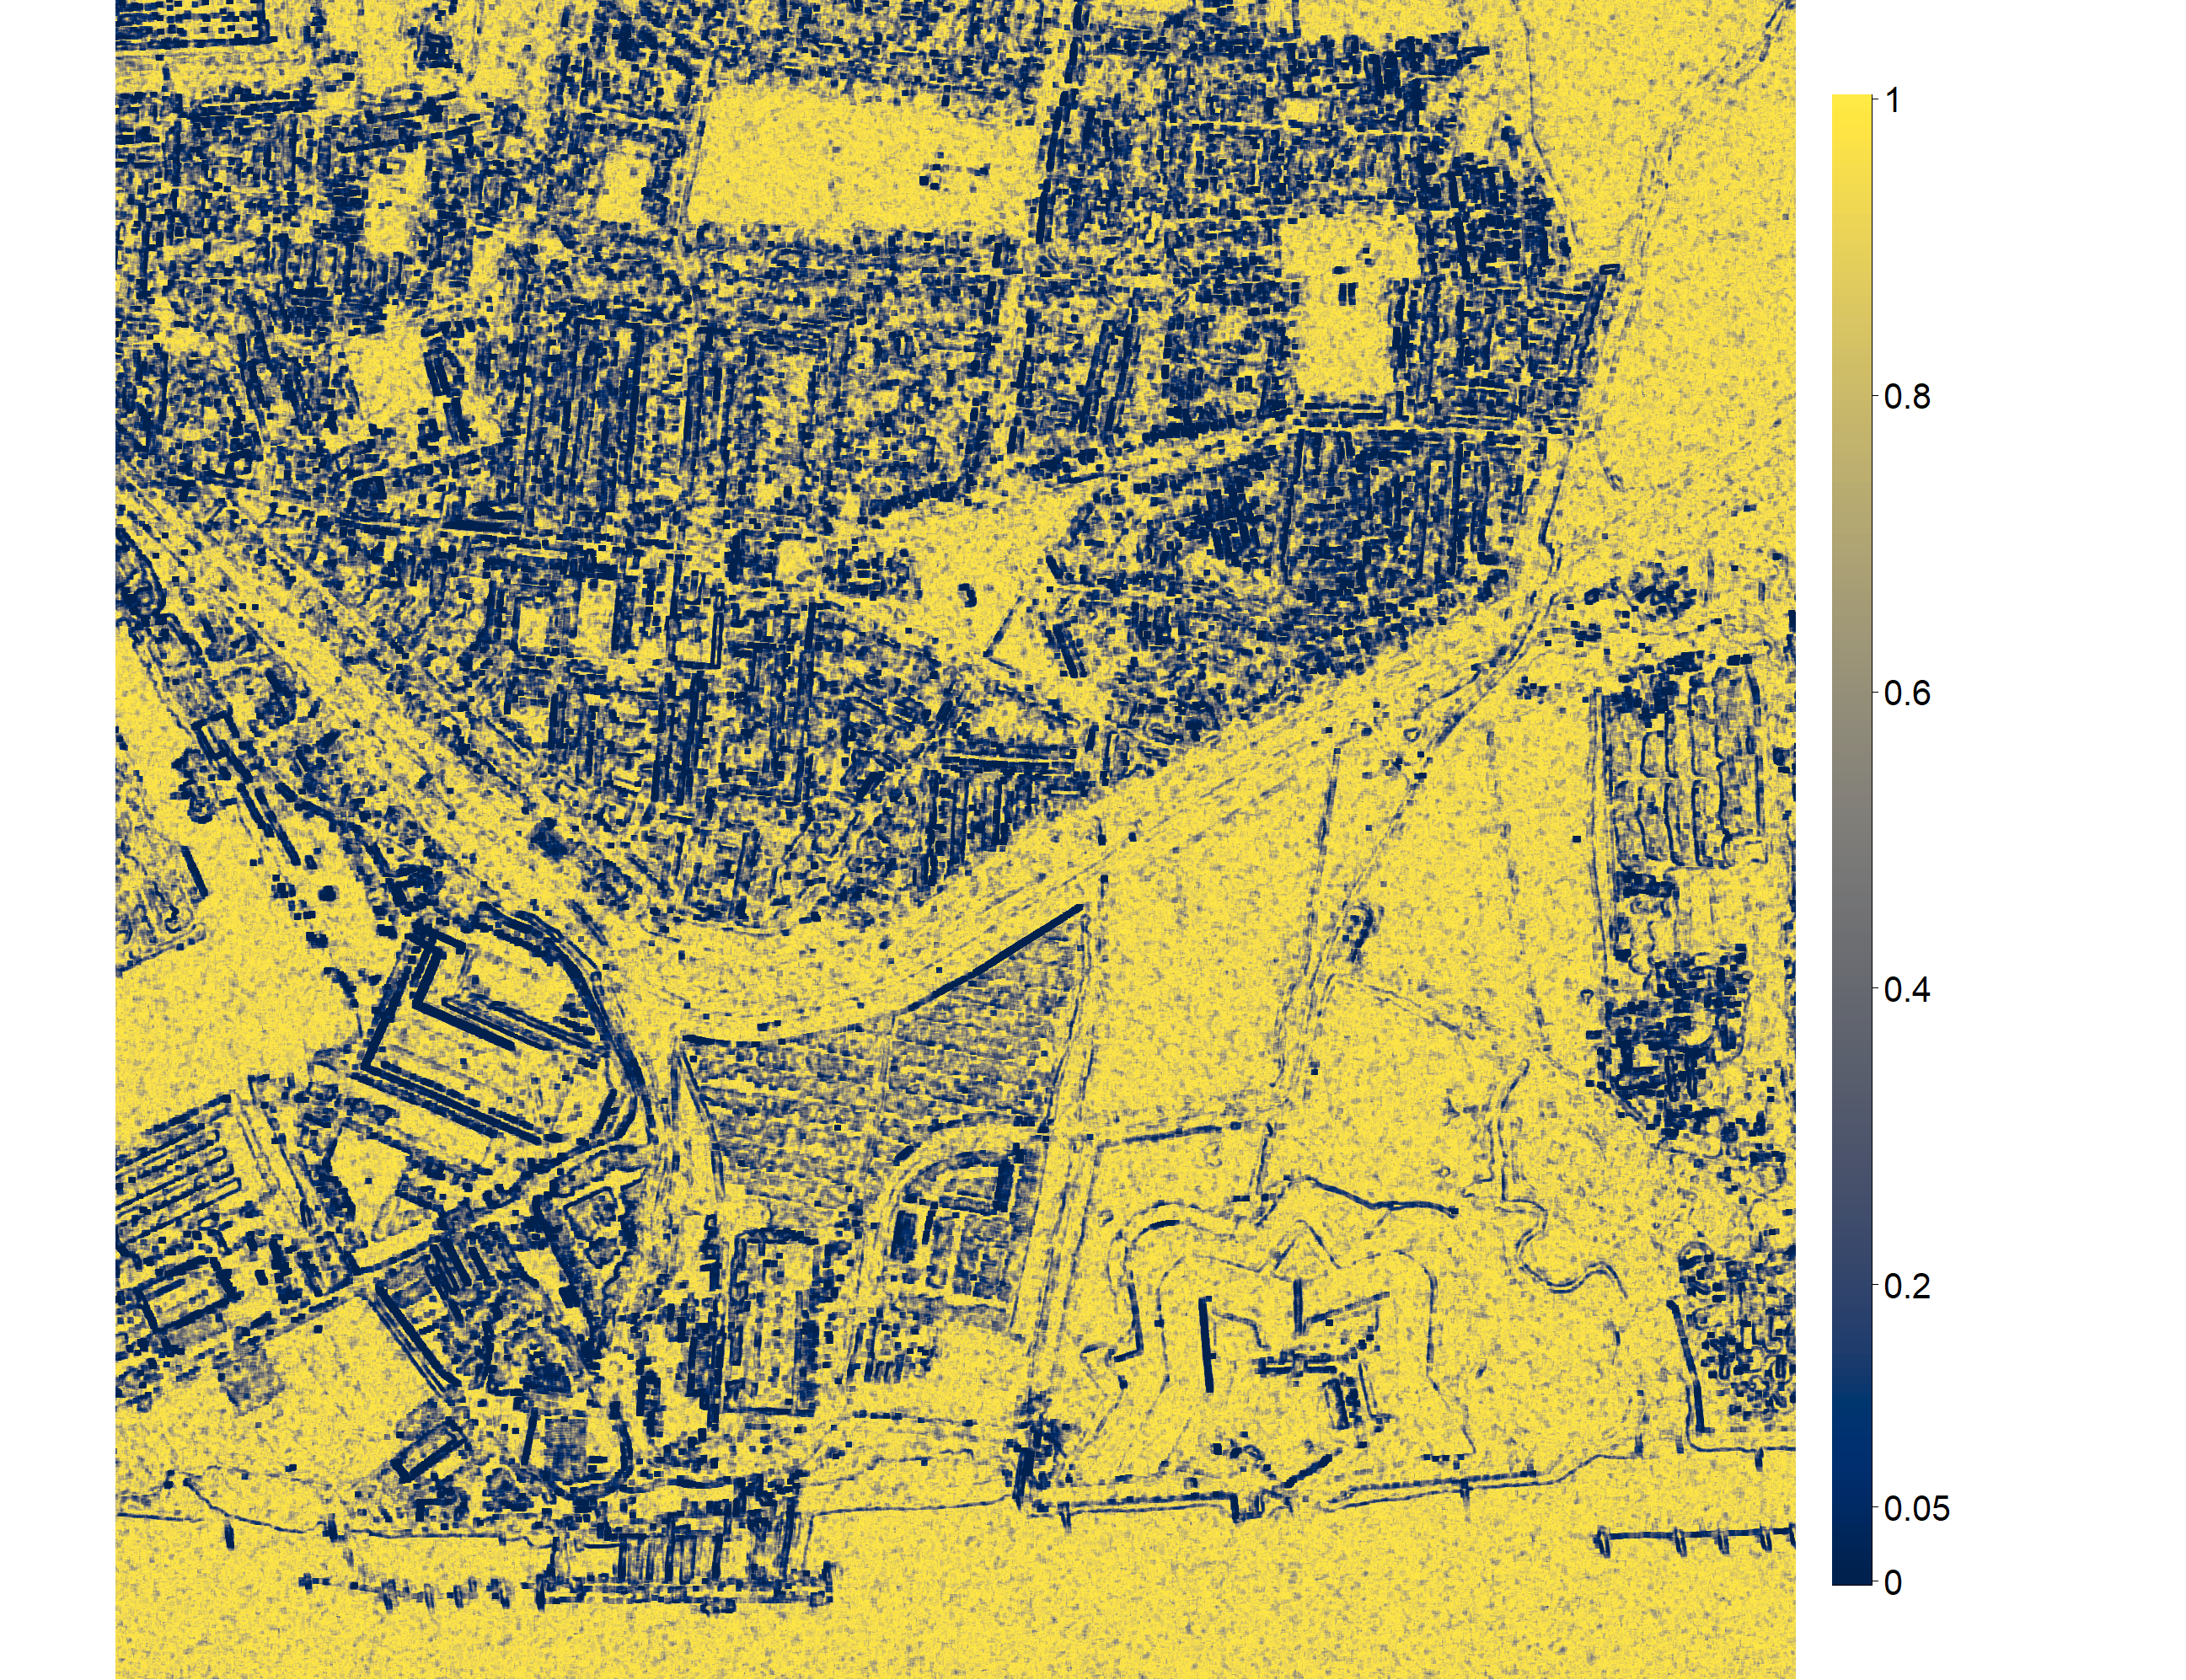
\includegraphics[width=\linewidth]{./Figures/H_pvalue_london_renyi.png}
%DIFDELCMD <         %%%
\DIFdelendFL \DIFaddbeginFL \DIFaddFL{\hspace{0.00001\textwidth}
    }\begin{subfigure}{0.142\textwidth}
        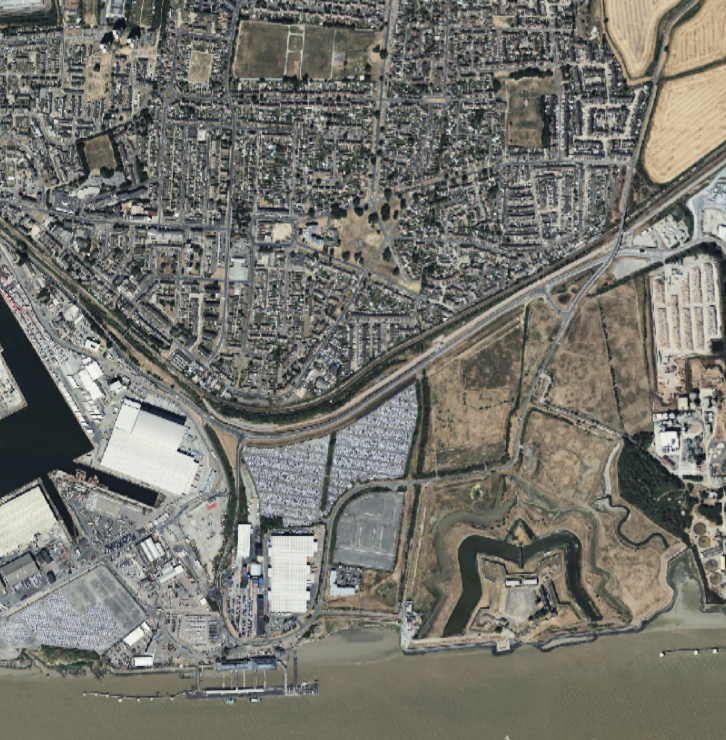
\includegraphics[width=\linewidth]{./Figures-R1/london_optical.png}
        \caption{\DIFaddFL{Optical image}}
        \label{fig:london-optical}
    \end{subfigure}
    \DIFaddFL{\hspace{0.00001\textwidth}
    }\begin{subfigure}{0.179\textwidth}
        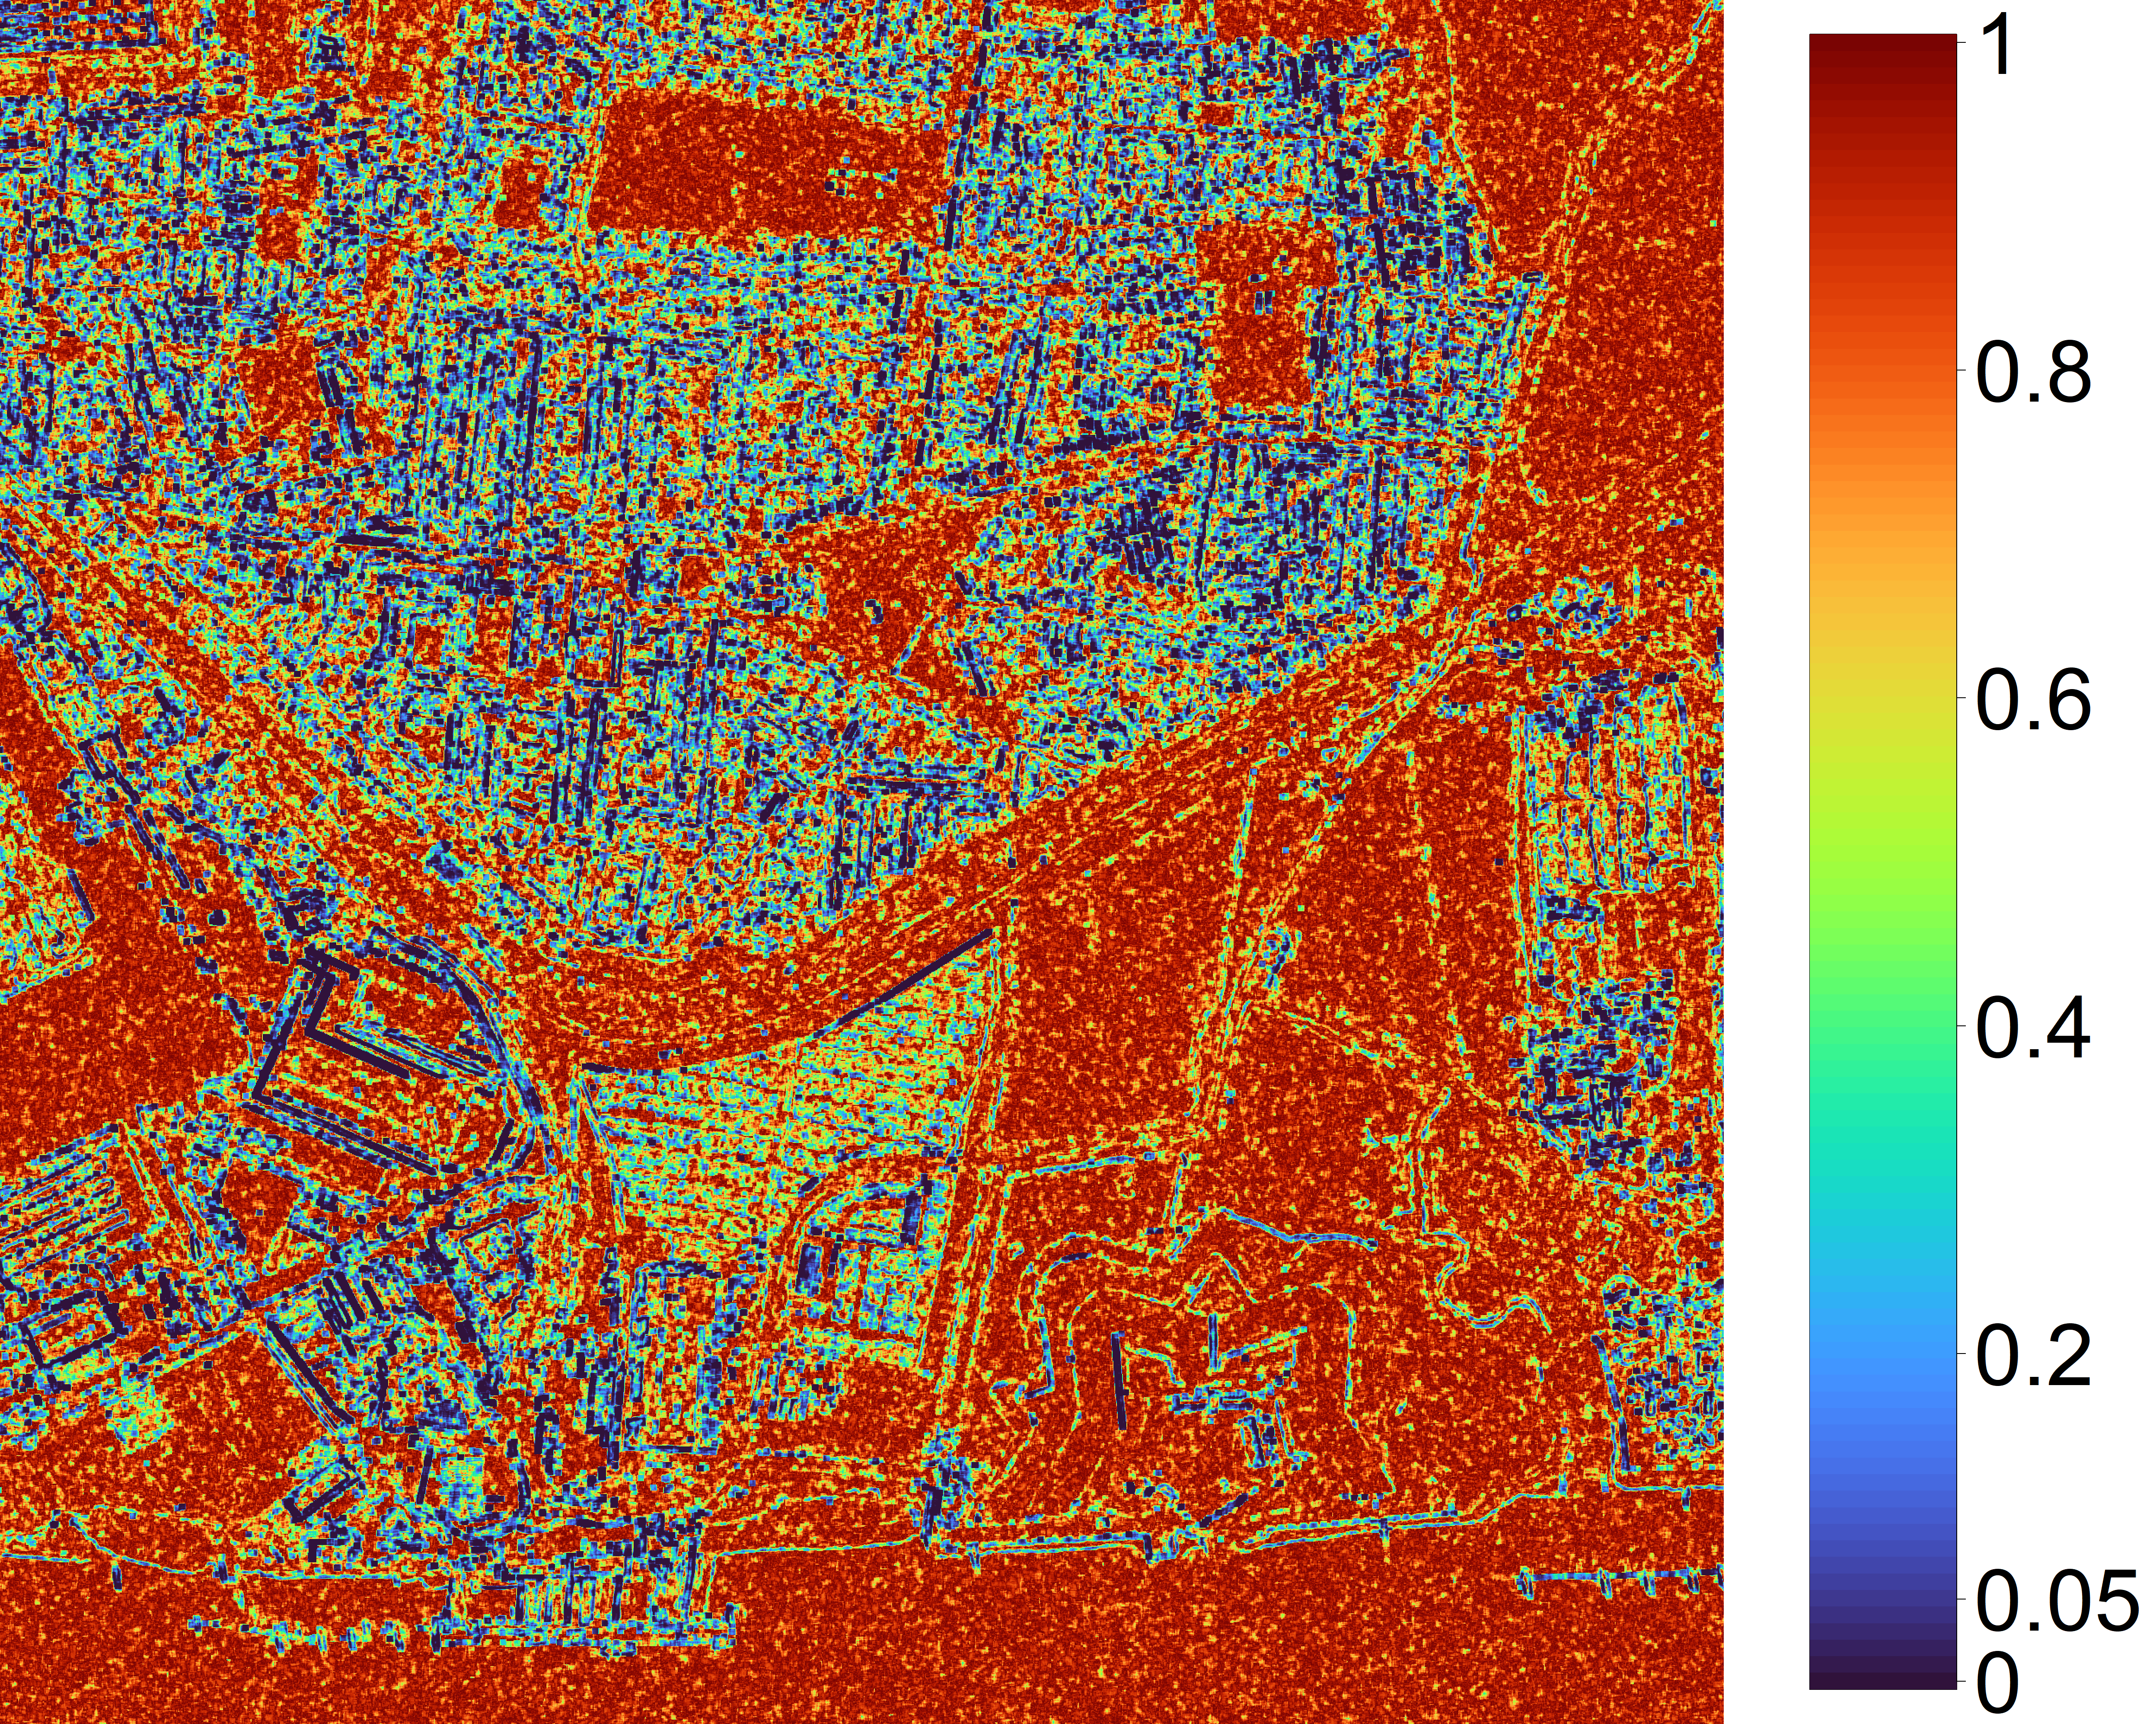
\includegraphics[width=\linewidth]{./Figures-R1/p-values_renyi-london_H1.png}
        \DIFaddendFL \caption{$p$-value map for $\small{S_{\widetilde{H}_{\lambda}}}$}
        \DIFdelbeginFL %DIFDELCMD < \label{fig:london-b}
%DIFDELCMD <     %%%
\DIFdelendFL \DIFaddbeginFL \label{fig:london-renyi}
    \DIFaddendFL \end{subfigure}
    \DIFdelbeginFL %DIFDELCMD < \begin{subfigure}{0.17\textwidth}
%DIFDELCMD <         \includegraphics[width=\linewidth]{./Figures/H_005_london_renyi_L1_.png}
%DIFDELCMD <         %%%
\DIFdelendFL \DIFaddbeginFL \DIFaddFL{\hspace{0.00001\textwidth}
    }\begin{subfigure}{0.145\textwidth}
        \includegraphics[width=\linewidth]{./Figures-R1/H_005_london_renyi_L1_.png}
        \DIFaddendFL \caption{Binary map for $\small{S_{\widetilde{H}_{\lambda}}}$}
        \DIFdelbeginFL %DIFDELCMD < \label{fig:london-c}
%DIFDELCMD <     %%%
\DIFdelendFL \DIFaddbeginFL \label{fig:london-005-renyi}
    \DIFaddendFL \end{subfigure}
   \DIFdelbeginFL %DIFDELCMD < \begin{subfigure}{0.22\textwidth}
%DIFDELCMD <         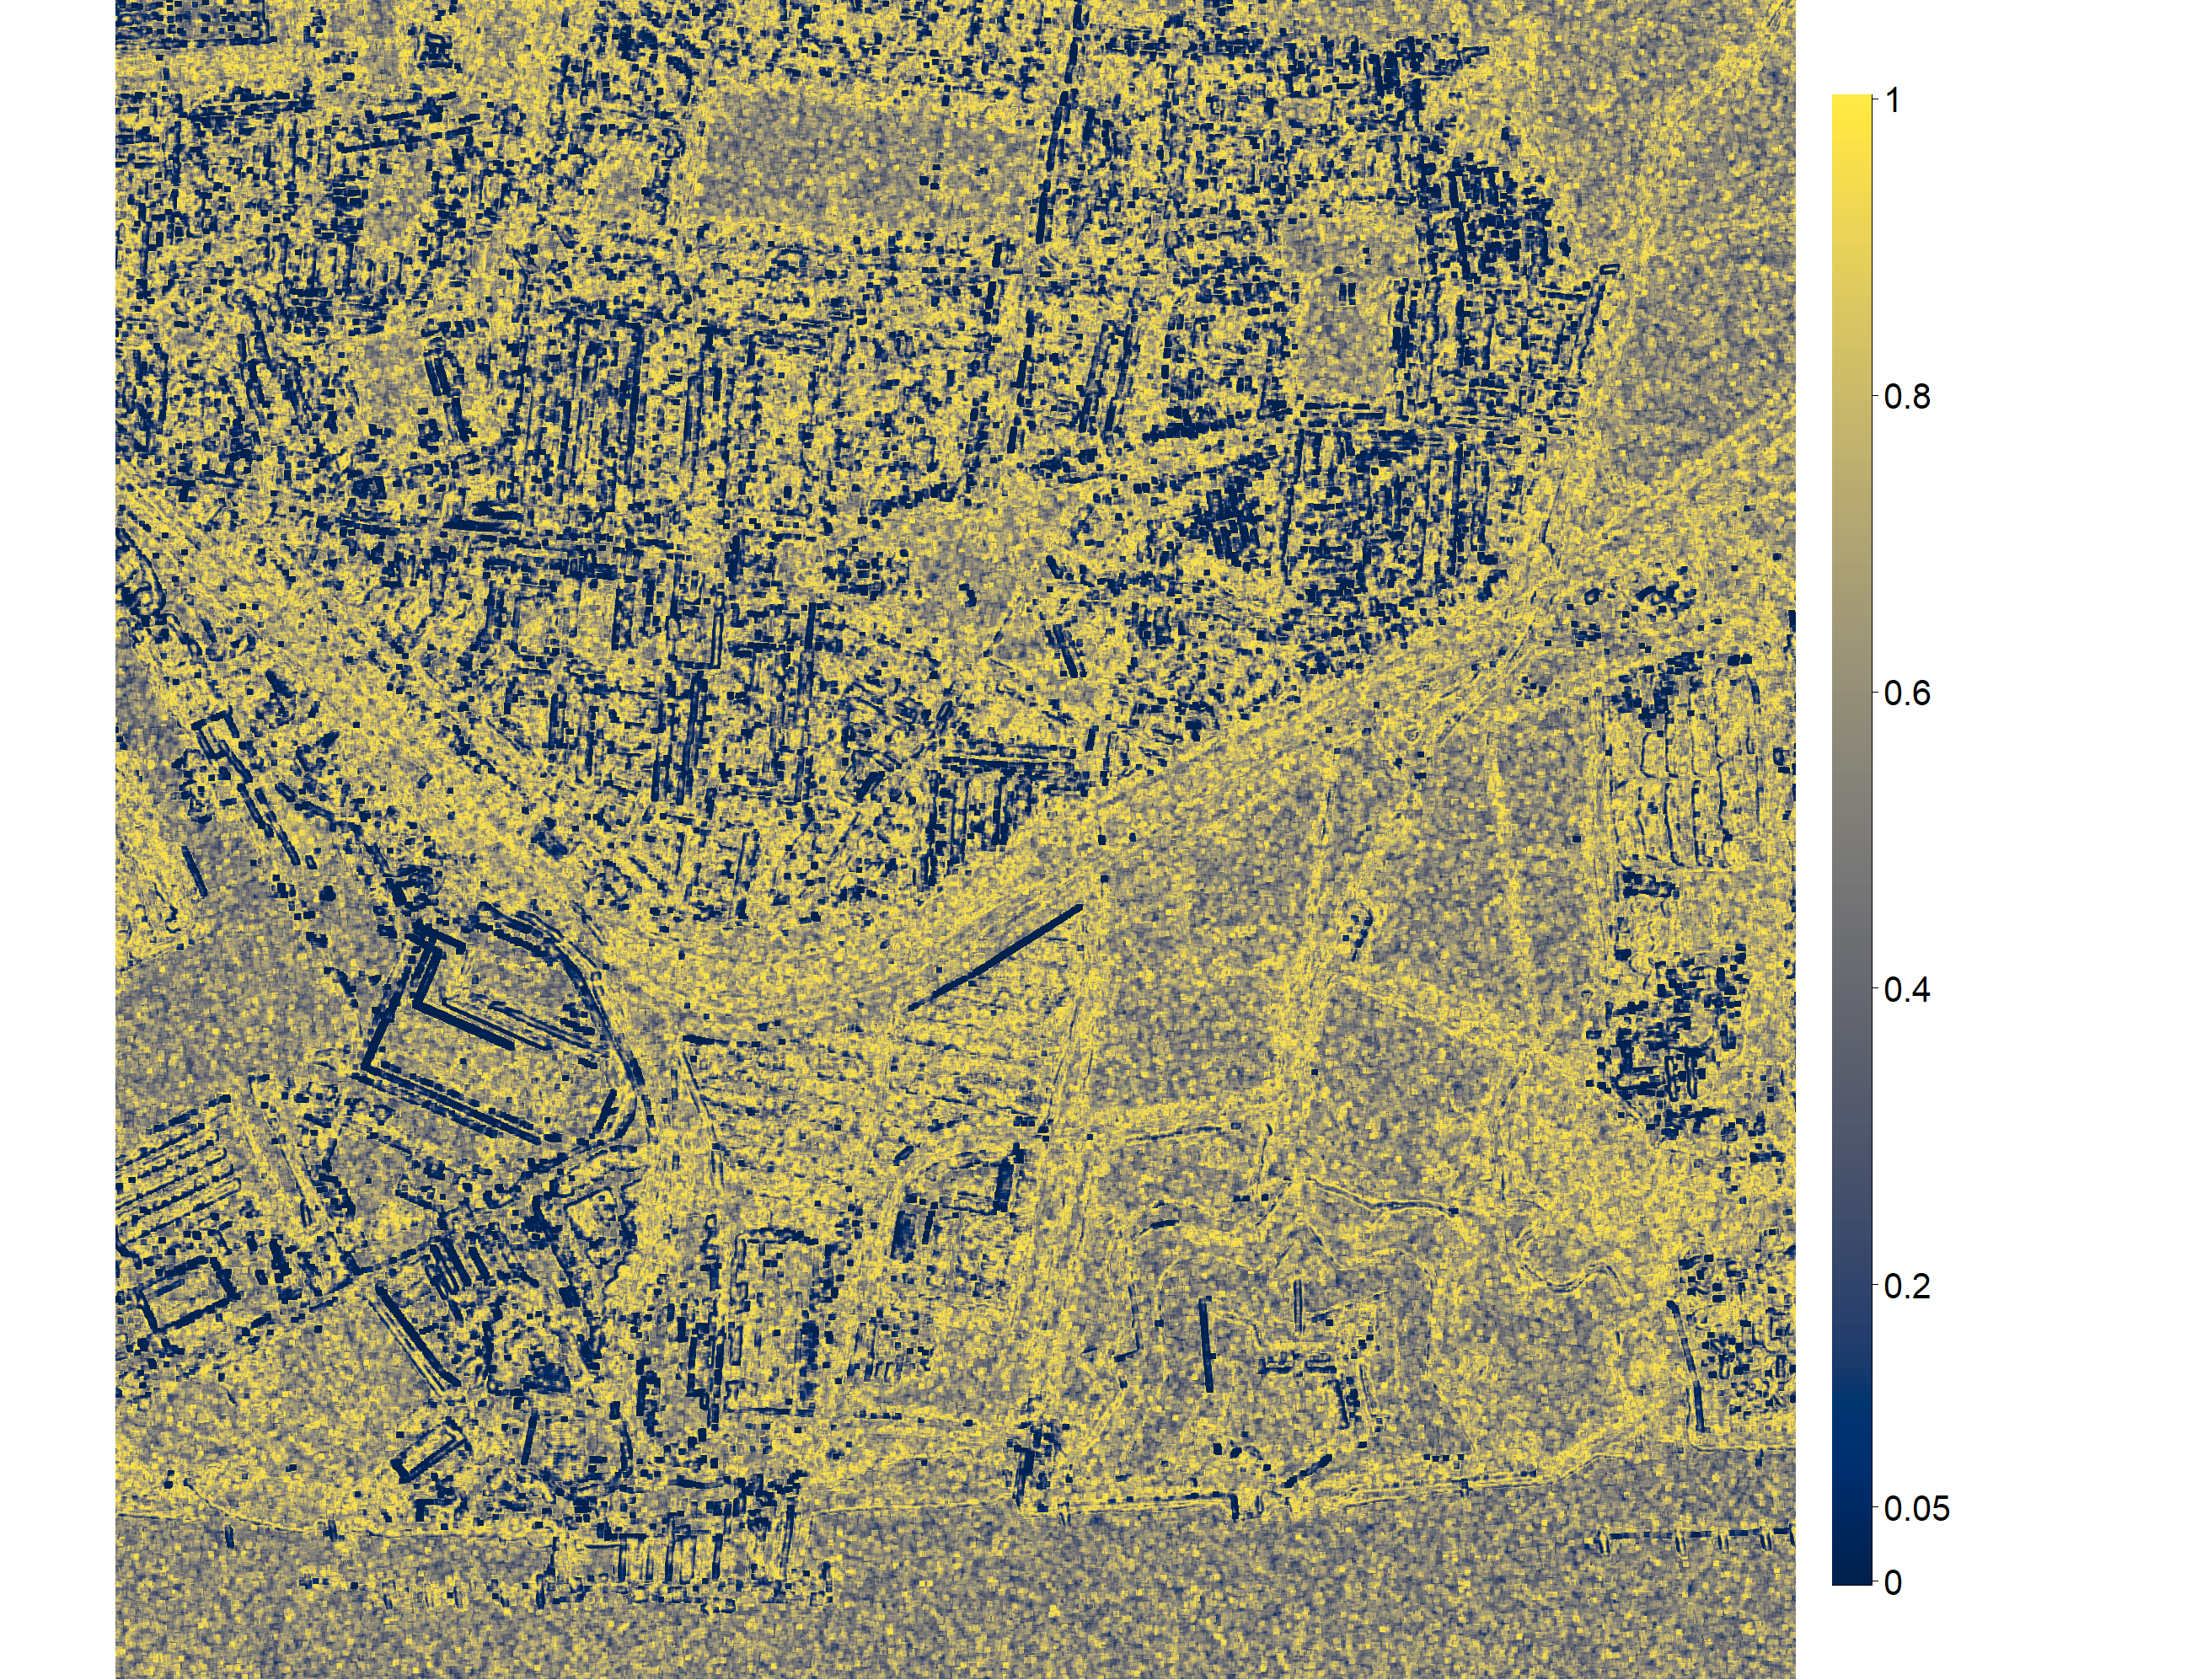
\includegraphics[width=\linewidth]{./Figures/H_pvalue_london_Shannon_c1.png}
%DIFDELCMD <         %%%
\DIFdelendFL \DIFaddbeginFL \DIFaddFL{\hspace{0.00001\textwidth}
    }\begin{subfigure}{0.18\textwidth}
        \includegraphics[width=\linewidth]{./Figures-R1/p-values_shannon-london_H1.png}
        \DIFaddendFL \caption{$p$-value map for $\tiny{S_{\widetilde{H}_{\text{AO}}}}$ }
        \DIFdelbeginFL %DIFDELCMD < \label{fig:london-d}
%DIFDELCMD <     %%%
\DIFdelendFL \DIFaddbeginFL \label{fig:london-shann}
    \DIFaddendFL \end{subfigure}
    \DIFdelbeginFL %DIFDELCMD < \begin{subfigure}{0.17\textwidth}
%DIFDELCMD <         \includegraphics[width=\linewidth]{./Figures/H_005_london_shannon.png}
%DIFDELCMD <         %%%
\DIFdelendFL \DIFaddbeginFL \DIFaddFL{\hspace{0.00001\textwidth}
    }\begin{subfigure}{0.145\textwidth}
        \includegraphics[width=\linewidth]{./Figures-R1/H_005_london_shannon.png}
        \DIFaddendFL \caption{Binary map for $\small{S_{\widetilde{H}_{\text{AO}}}}$}
        \DIFdelbeginFL %DIFDELCMD < \label{fig:london-e}
%DIFDELCMD <     %%%
\DIFdelendFL \DIFaddbeginFL \label{fig:london-005-shann}
    \DIFaddendFL \end{subfigure}
    \caption{Detection of heterogeneous areas in a SAR image over London, UK: comparison with the tests $\small{S_{\widetilde{H}_{\lambda}}}$ and $\small{S_{\widetilde{H}_{\text{AO}}}}$.}
    \label{fig:london}
\end{figure*}

\begin{figure*}[hbt]
    \centering
        \DIFdelbeginFL %DIFDELCMD < \begin{subfigure}{0.17\textwidth}
%DIFDELCMD <         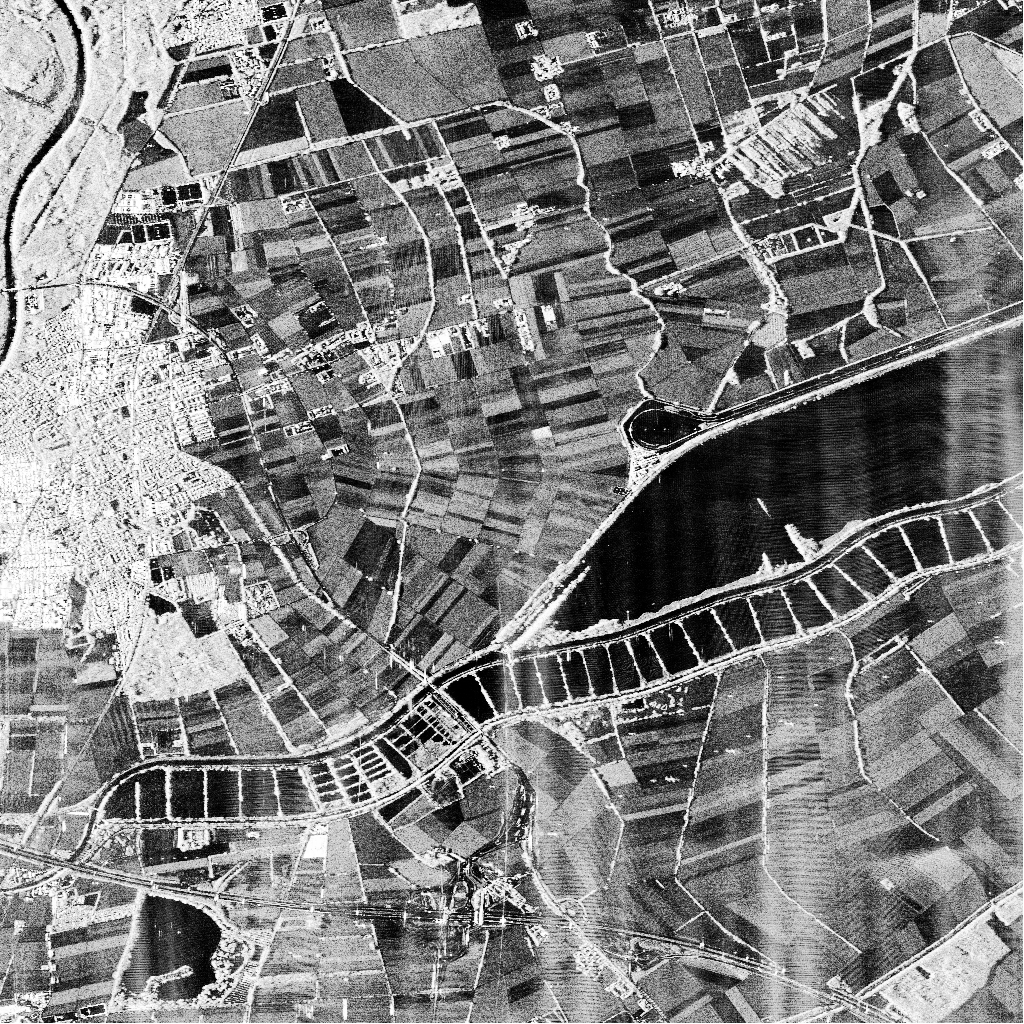
\includegraphics[width=\linewidth]{./Figures/munich_1024_2.png}
%DIFDELCMD <         %%%
\DIFdelendFL \DIFaddbeginFL \begin{subfigure}{0.145\textwidth}
        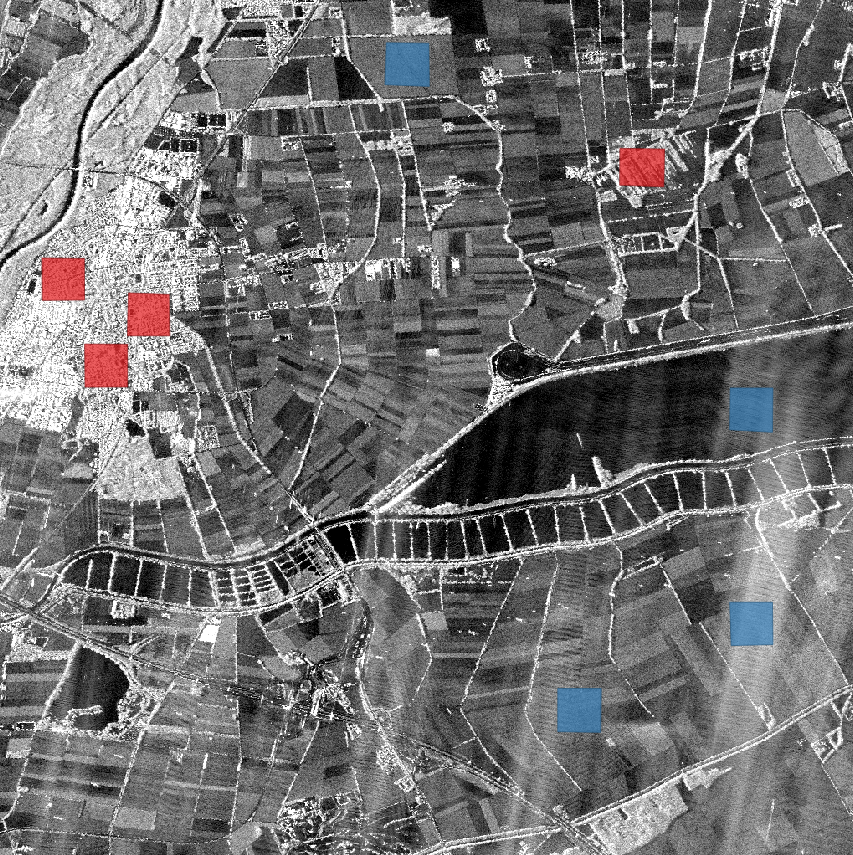
\includegraphics[width=\linewidth]{./Figures-R1/munich_roi.png}
        \DIFaddendFL \caption{SAR image}
        \DIFdelbeginFL %DIFDELCMD < \label{fig:munich-a}
%DIFDELCMD <     %%%
\DIFdelendFL \DIFaddbeginFL \label{fig:munich-sar}
    \DIFaddendFL \end{subfigure}
    \DIFdelbeginFL %DIFDELCMD < \begin{subfigure}{0.23\textwidth}
%DIFDELCMD <         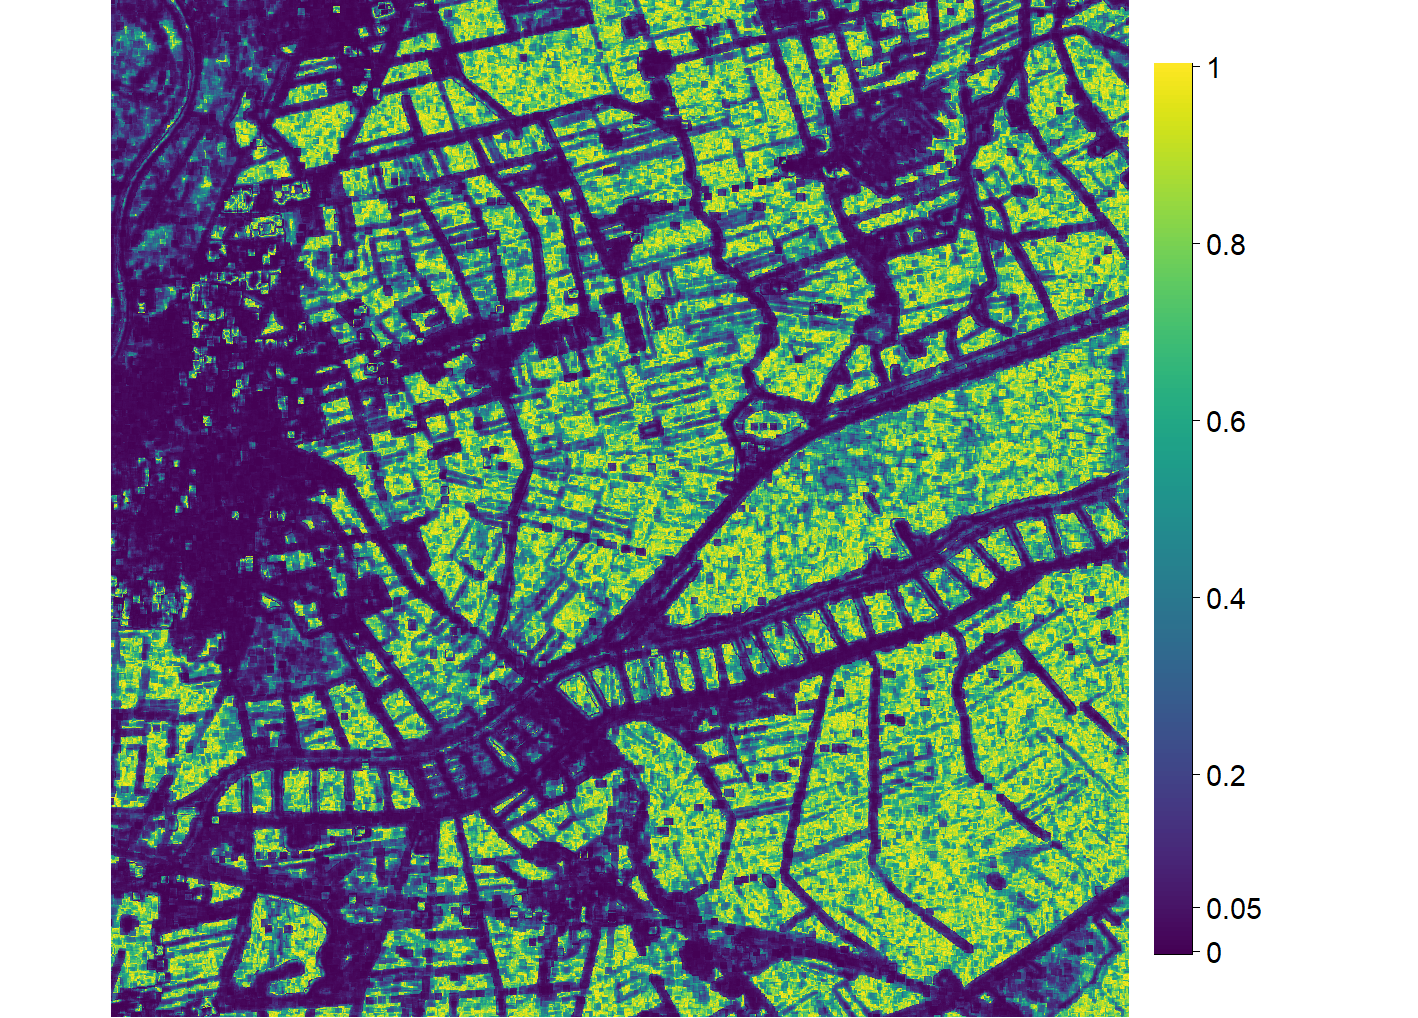
\includegraphics[width=\linewidth]{./Figures/H_pvalue_muni_renyi.png}
%DIFDELCMD <         %%%
\DIFdelendFL \DIFaddbeginFL \DIFaddFL{\hspace{0.00001\textwidth}
  }\begin{subfigure}{0.137\textwidth}
        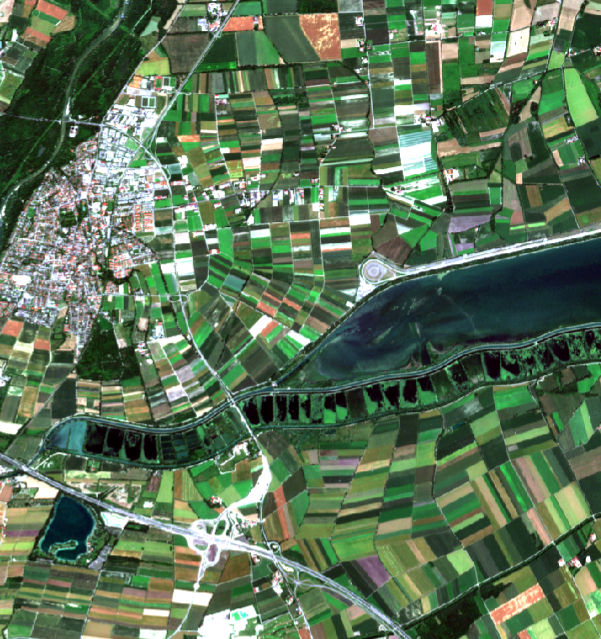
\includegraphics[width=\linewidth]{./Figures-R1/munich_optical.png}
        \caption{\DIFaddFL{Optical image}}
        \label{fig:munich-optical}
    \end{subfigure}
    \DIFaddFL{\hspace{0.00001\textwidth}
    }\begin{subfigure}{0.178\textwidth}
        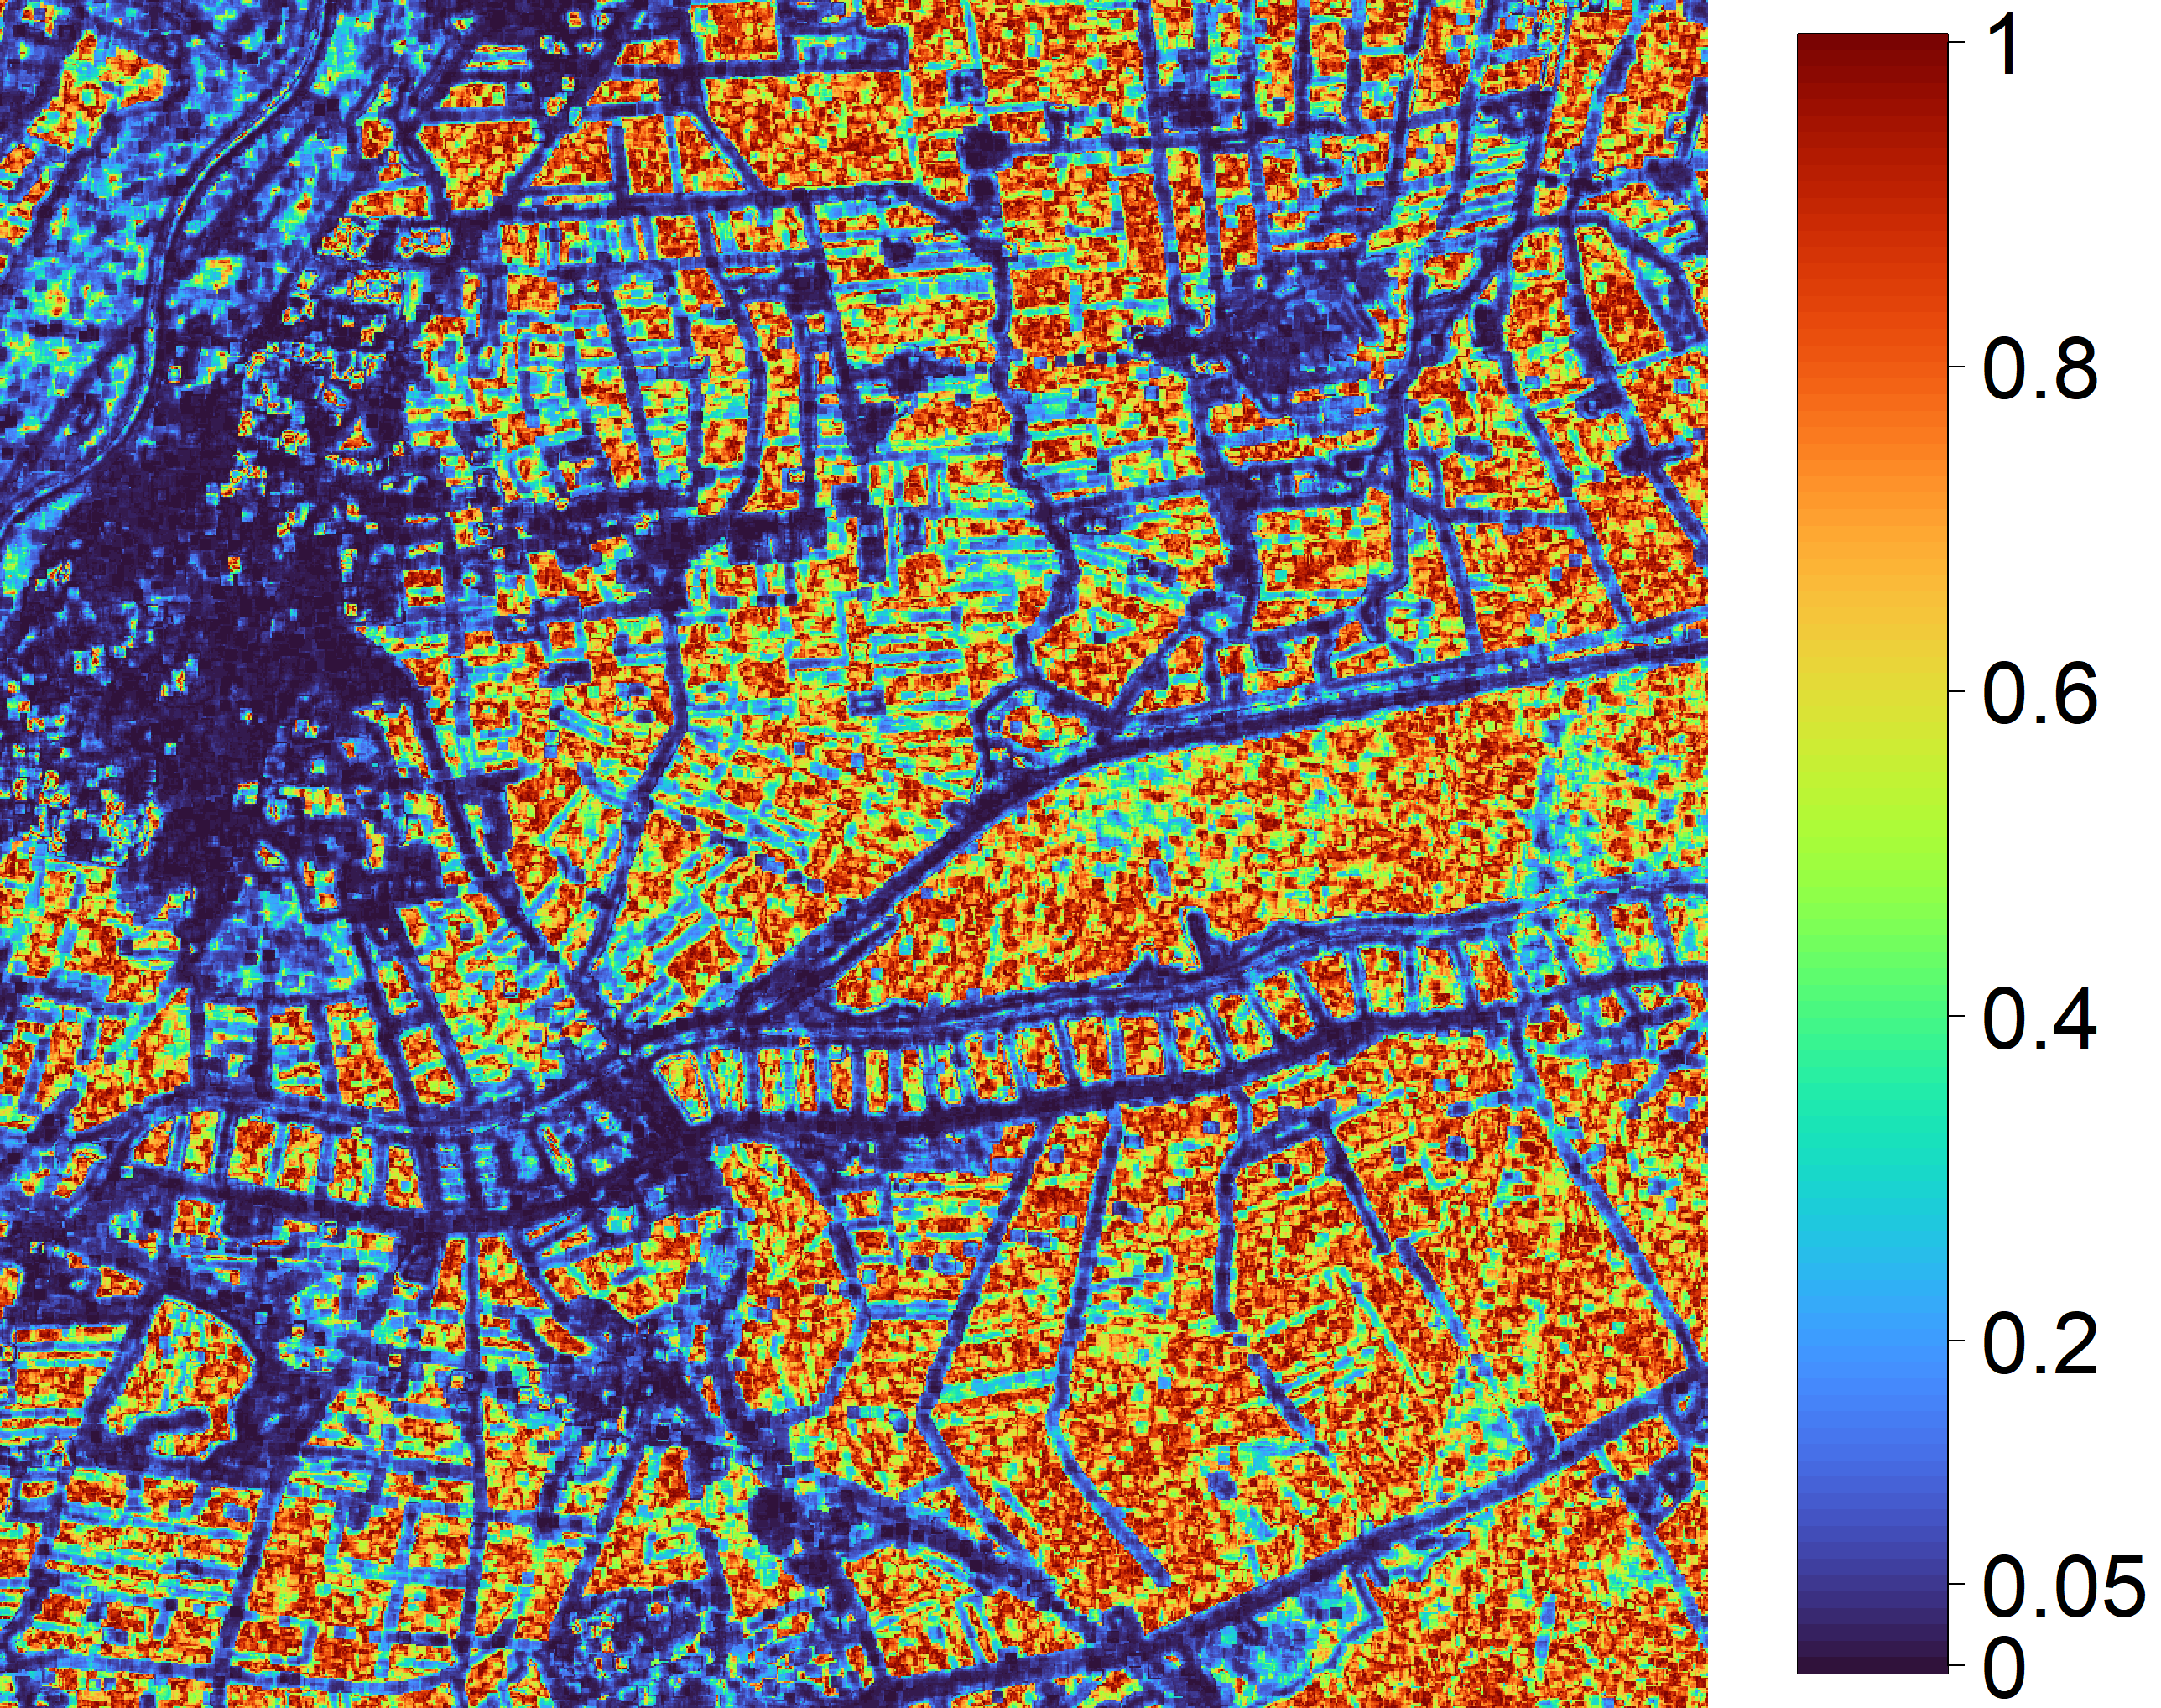
\includegraphics[width=\linewidth]{./Figures-R1/p-values_renyi-munich_H.png}
        \DIFaddendFL \caption{$p$-value map for $\small{S_{\widetilde{H}_{\lambda}}}$}
        \DIFdelbeginFL %DIFDELCMD < \label{fig:munich-b}
%DIFDELCMD <     %%%
\DIFdelendFL \DIFaddbeginFL \label{fig:munich-renyi}
    \DIFaddendFL \end{subfigure}
    \DIFdelbeginFL %DIFDELCMD < \begin{subfigure}{0.16\textwidth}
%DIFDELCMD <         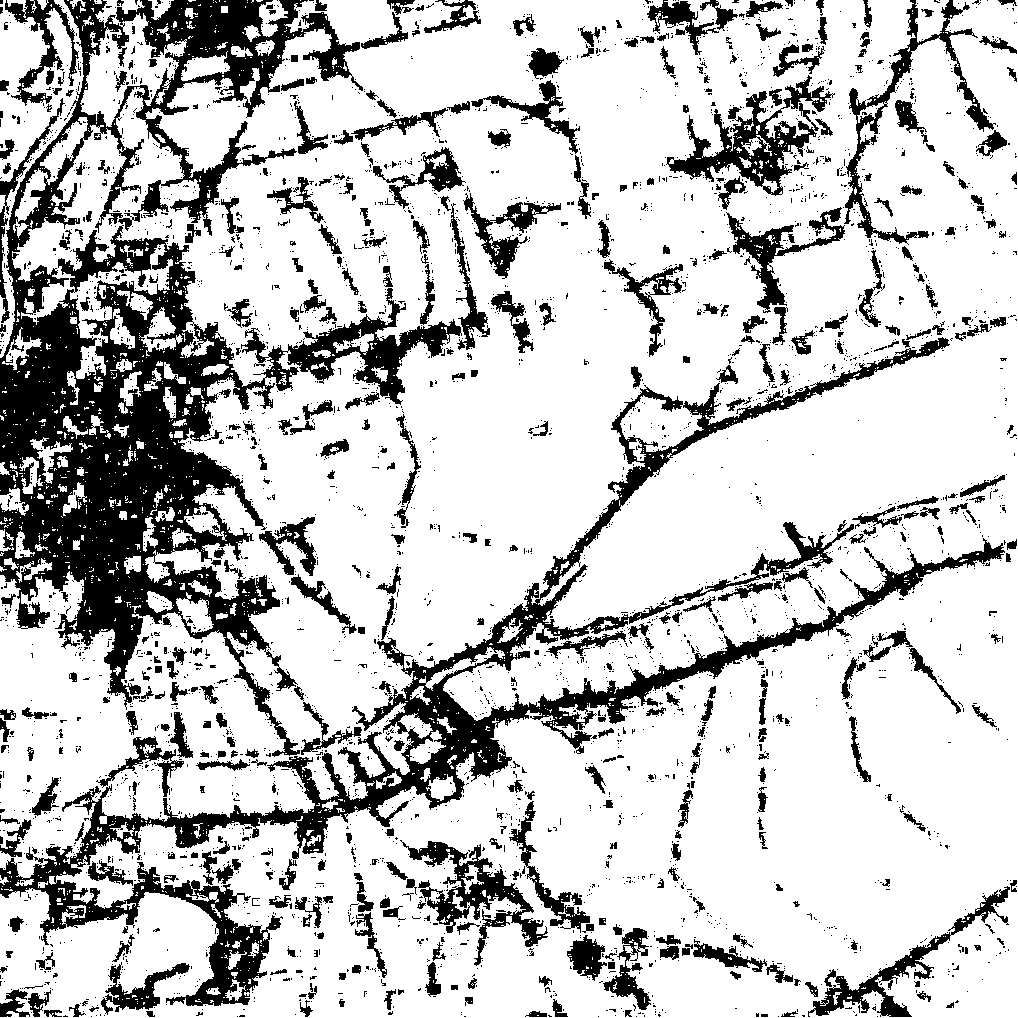
\includegraphics[width=\linewidth]{./Figures/H_005_munich_renyi.png}
%DIFDELCMD <         %%%
\DIFdelendFL \DIFaddbeginFL \DIFaddFL{\hspace{0.00001\textwidth}
    }\begin{subfigure}{0.144\textwidth}
        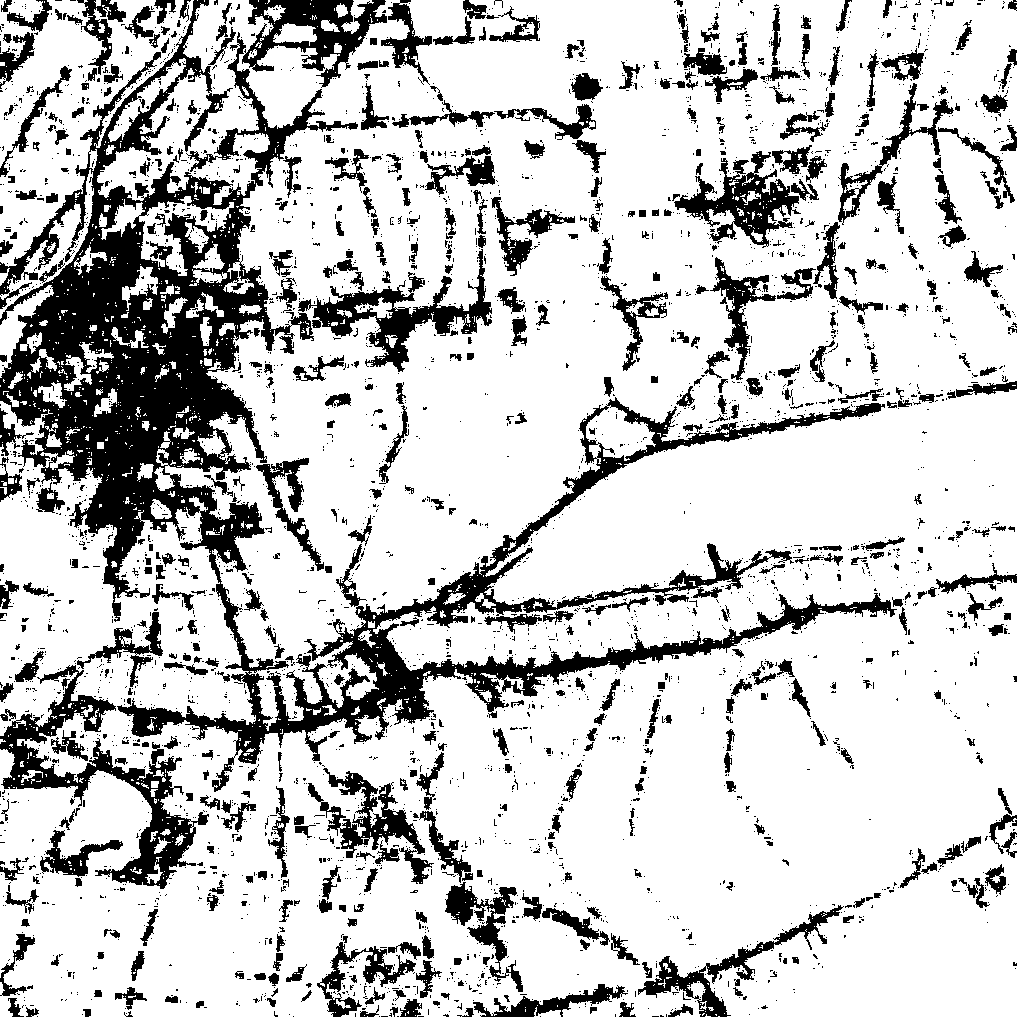
\includegraphics[width=\linewidth]{./Figures-R1/H_005_renyi_munich.png}
        \DIFaddendFL \caption{Binary map for $\small{S_{\widetilde{H}_{\lambda}}}$}
        \DIFdelbeginFL %DIFDELCMD < \label{fig:munich-c}
%DIFDELCMD <     %%%
\DIFdelendFL \DIFaddbeginFL \label{fig:munich-005-renyi}
    \DIFaddendFL \end{subfigure}
    \DIFdelbeginFL %DIFDELCMD < \begin{subfigure}{0.23\textwidth}
%DIFDELCMD <         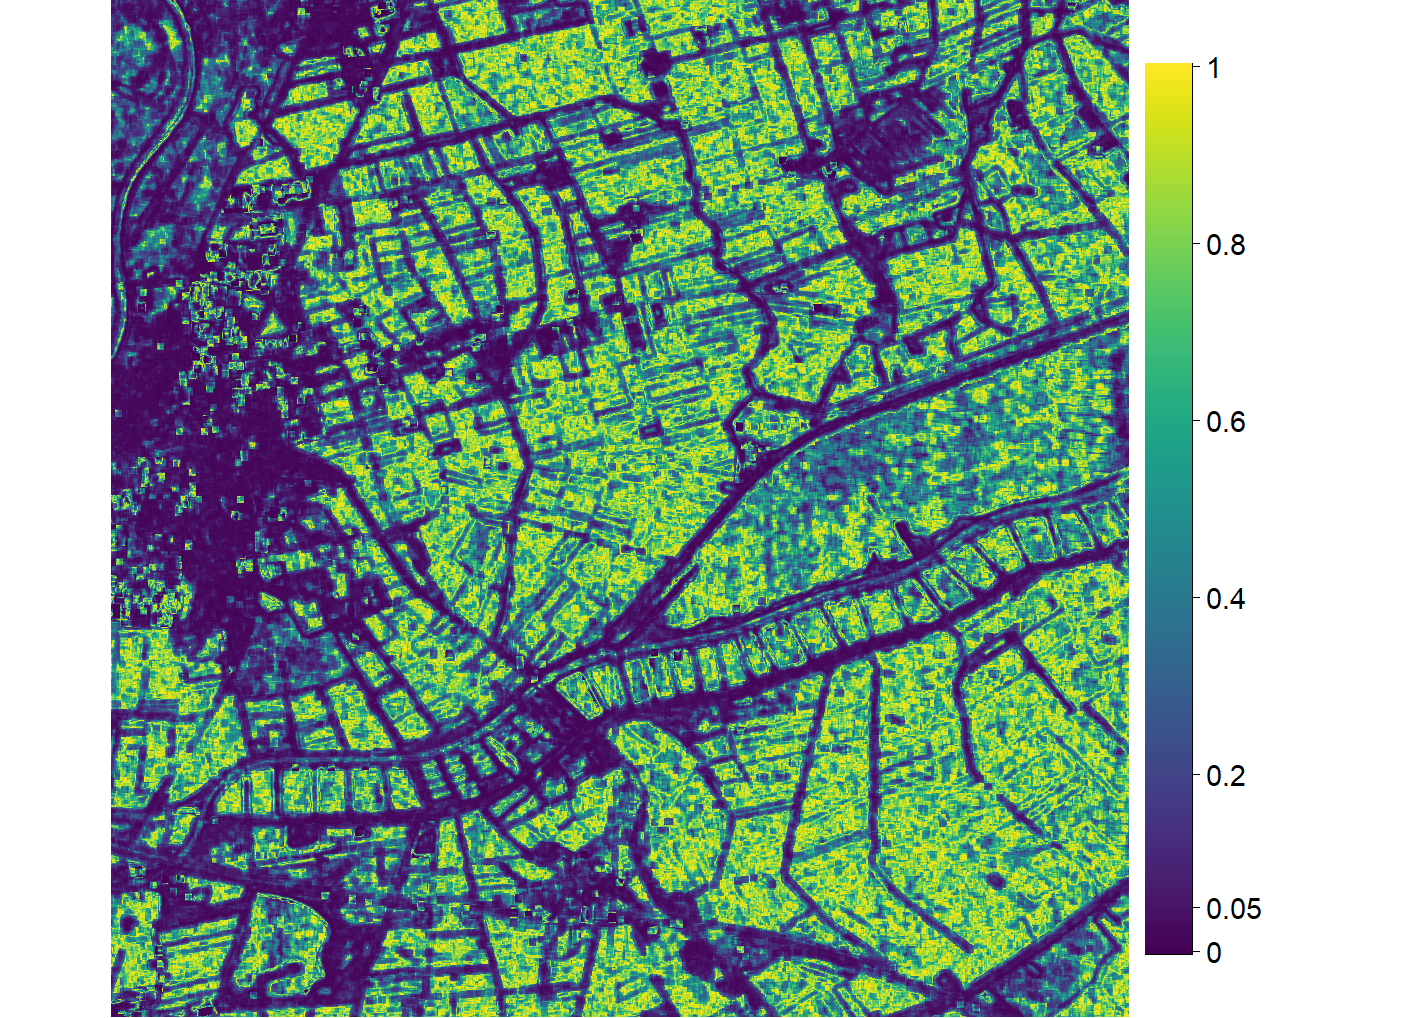
\includegraphics[width=\linewidth]{./Figures/H_pvalue_muni_Shan22.png}
%DIFDELCMD <         %%%
\DIFdelendFL \DIFaddbeginFL \DIFaddFL{\hspace{0.00001\textwidth}
    }\begin{subfigure}{0.178\textwidth}
        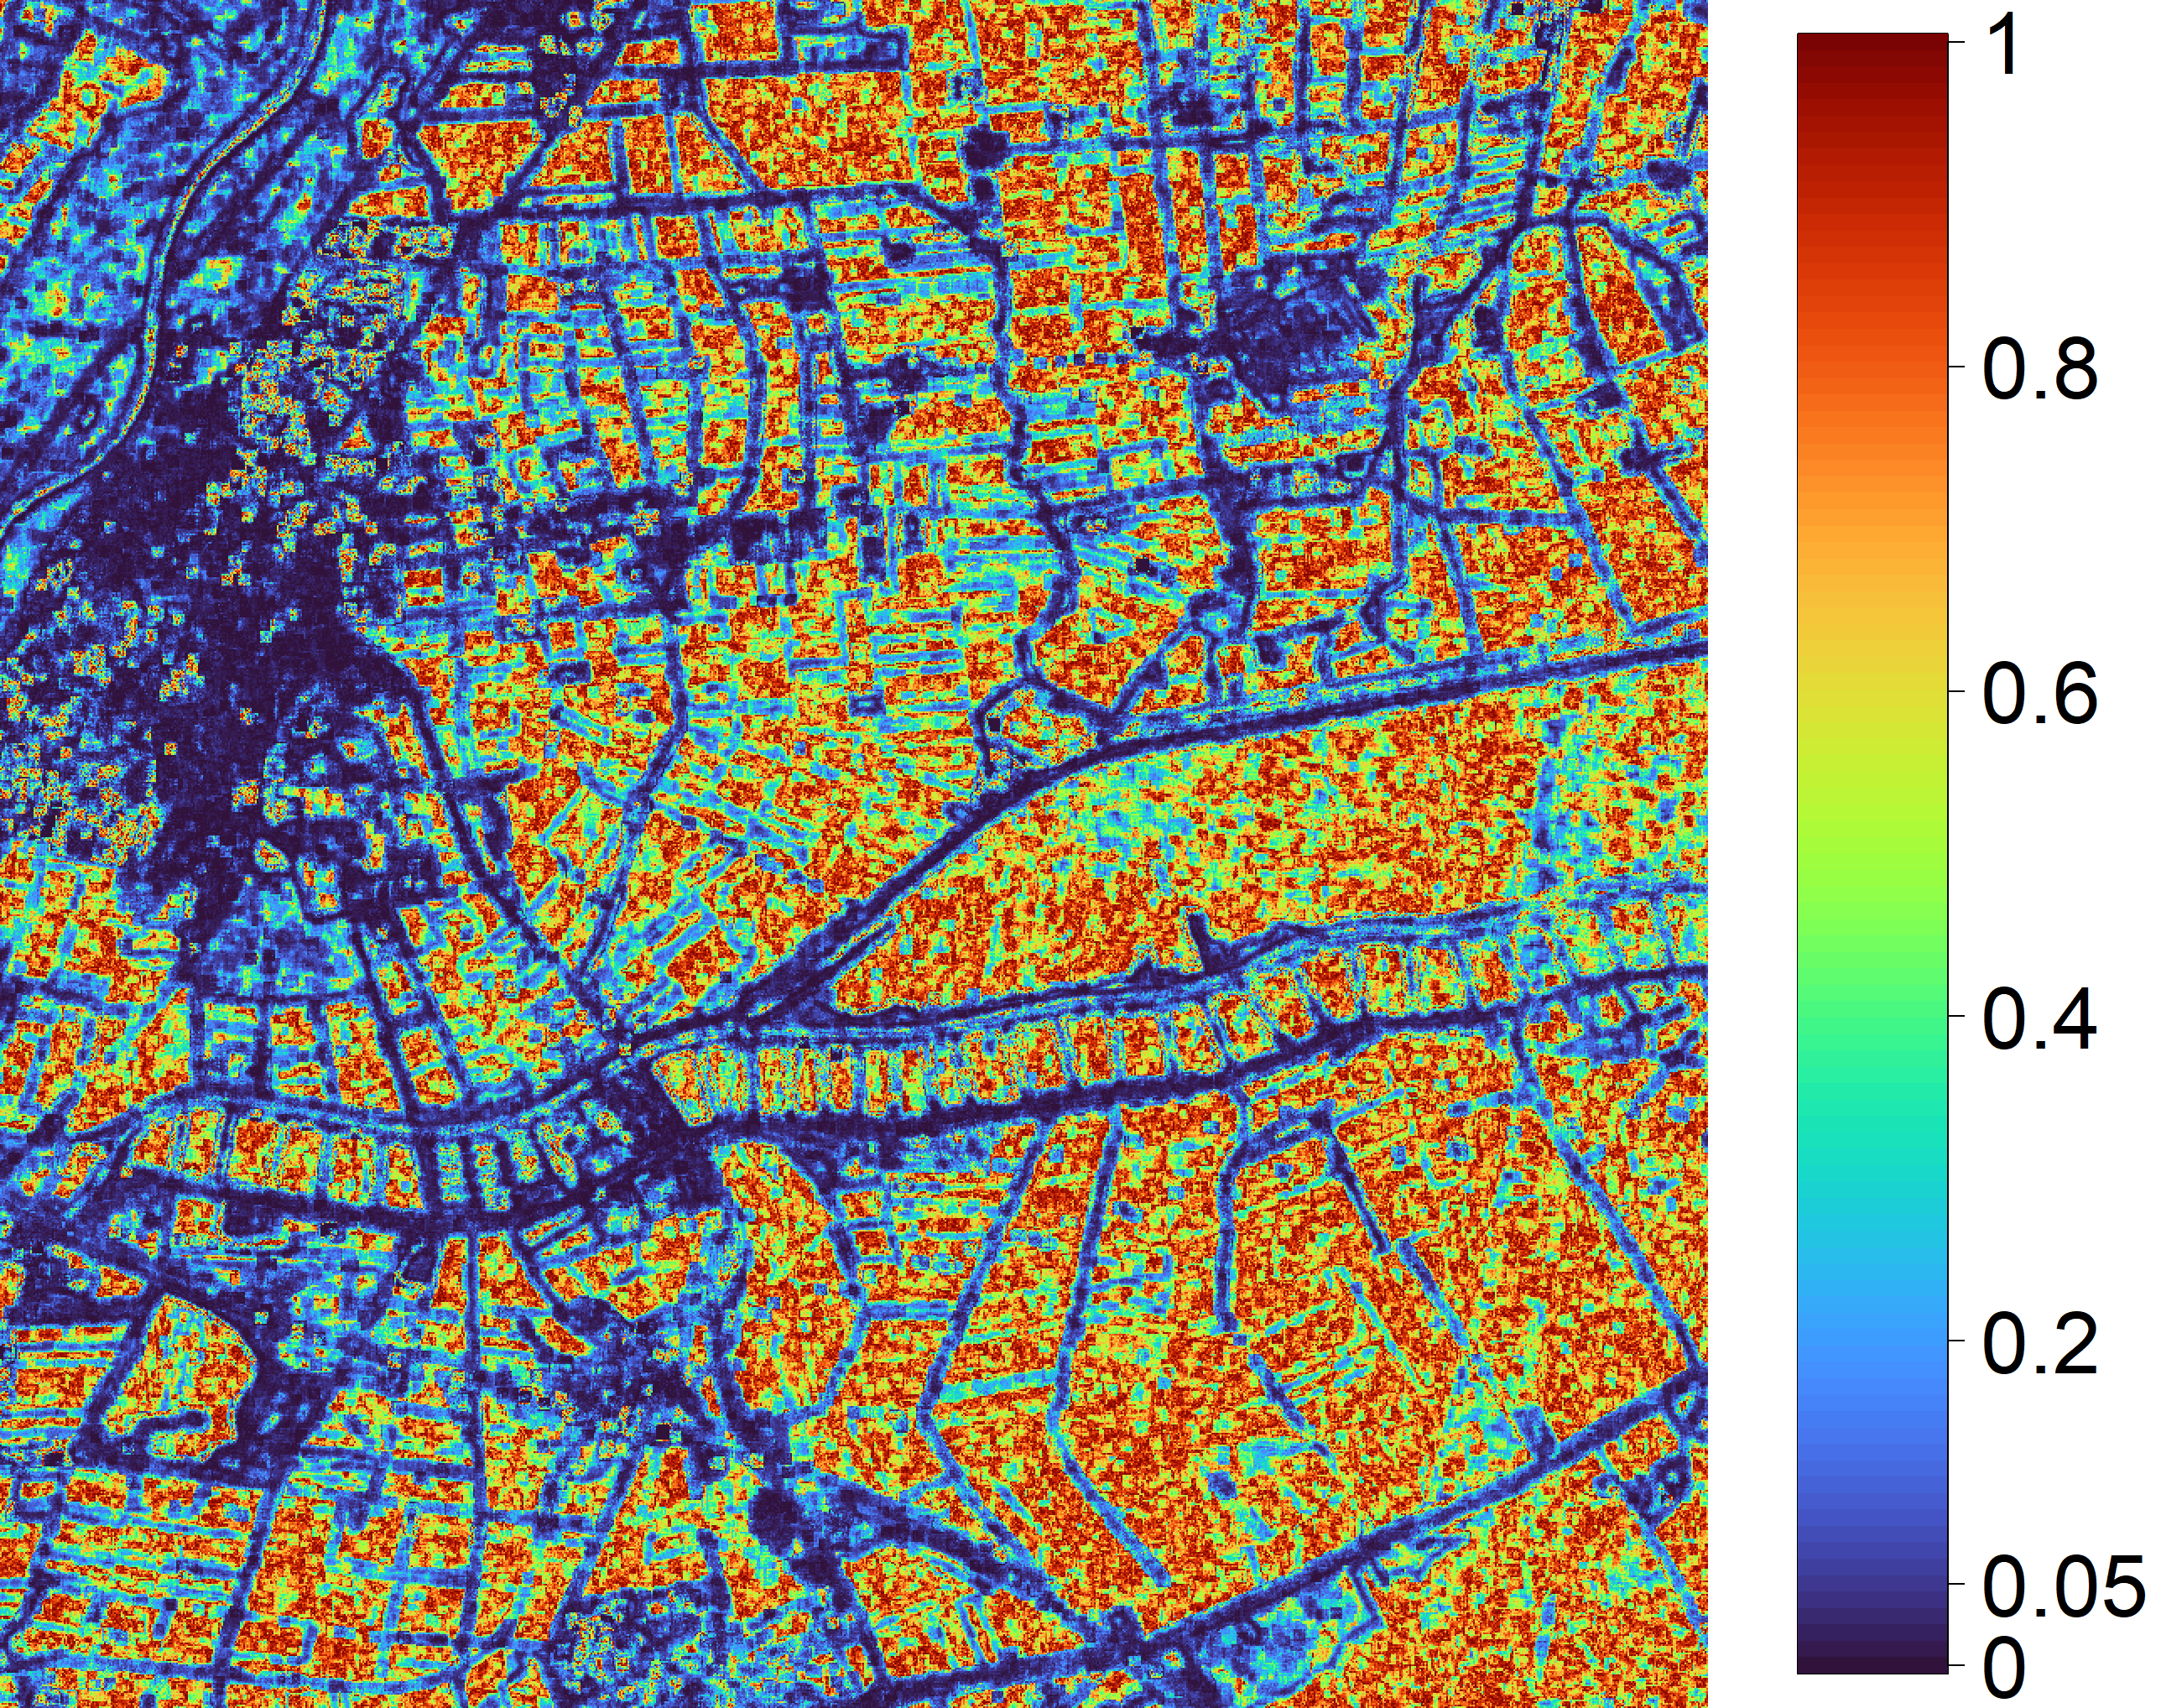
\includegraphics[width=\linewidth]{./Figures-R1/p-values_shannon-munich_H.png}
        \DIFaddendFL \caption{$p$-value map for $S_{\widetilde{H}_{\text{AO}}}$}
        \DIFdelbeginFL %DIFDELCMD < \label{fig:munich-d}
%DIFDELCMD <     %%%
\DIFdelendFL \DIFaddbeginFL \label{fig:munich-shann}
    \DIFaddendFL \end{subfigure}
   \DIFdelbeginFL %DIFDELCMD < \begin{subfigure}{0.16\textwidth}
%DIFDELCMD <         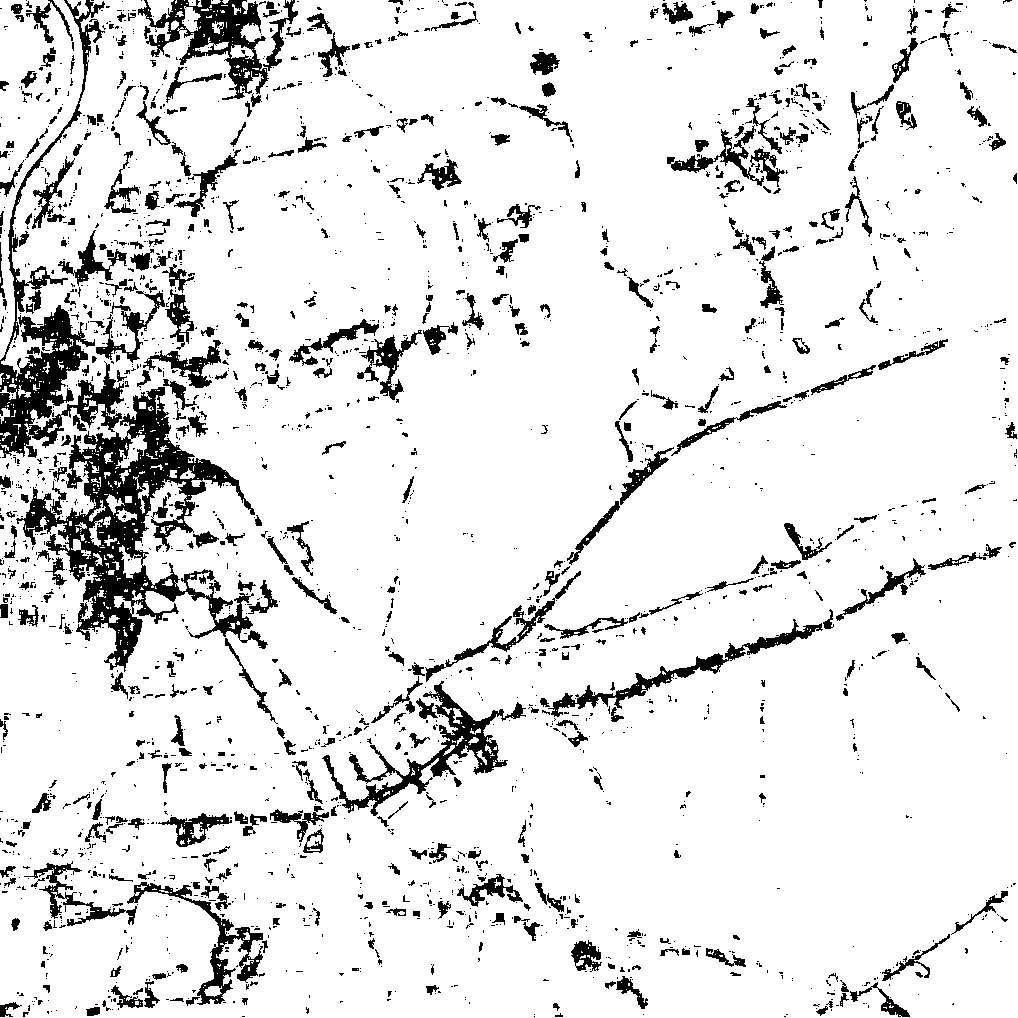
\includegraphics[width=\linewidth]{./Figures/H_005_munich_sh_AO_L12.png}
%DIFDELCMD <         %%%
\DIFdelendFL \DIFaddbeginFL \DIFaddFL{\hspace{0.00001\textwidth}
    }\begin{subfigure}{0.144\textwidth}
        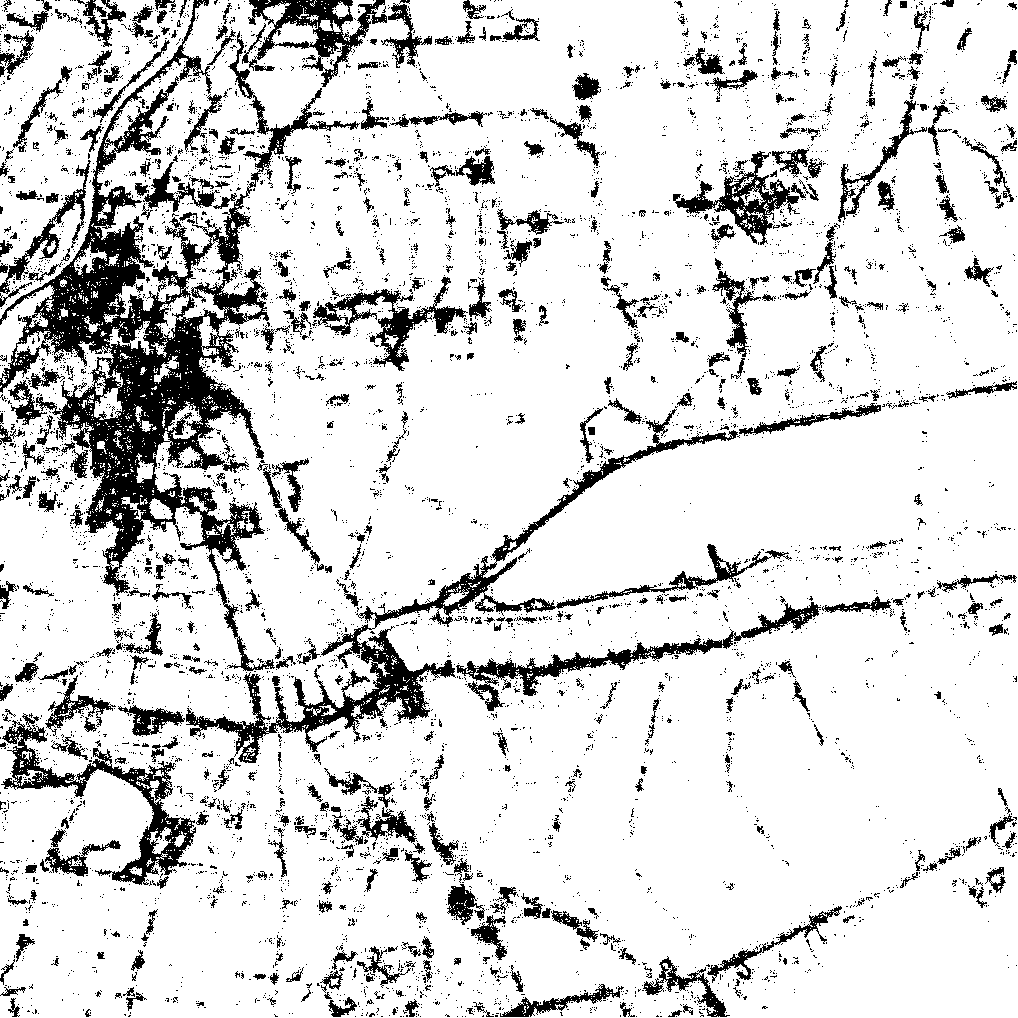
\includegraphics[width=\linewidth]{./Figures-R1/H_005_shannon_munich.png}
        \DIFaddendFL \caption{Binary map for $\small{S_{\widetilde{H}_{\text{AO}}}}$}
        \DIFdelbeginFL %DIFDELCMD < \label{fig:munich-e}
%DIFDELCMD <     %%%
\DIFdelendFL \DIFaddbeginFL \label{fig:munich-005-shann}
    \DIFaddendFL \end{subfigure}
    \caption{Detection of heterogeneous areas in a SAR image over Munich, Germany: comparison with the tests $\small{S_{\widetilde{H}_{\lambda}}}$ and $\small{S_{\widetilde{H}_{\text{AO}}}}$.}
    \label{fig:munich}
\end{figure*}

\begin{figure*}[hbt]
    \centering
        \DIFdelbeginFL %DIFDELCMD < \begin{subfigure}{0.16\textwidth}
%DIFDELCMD <         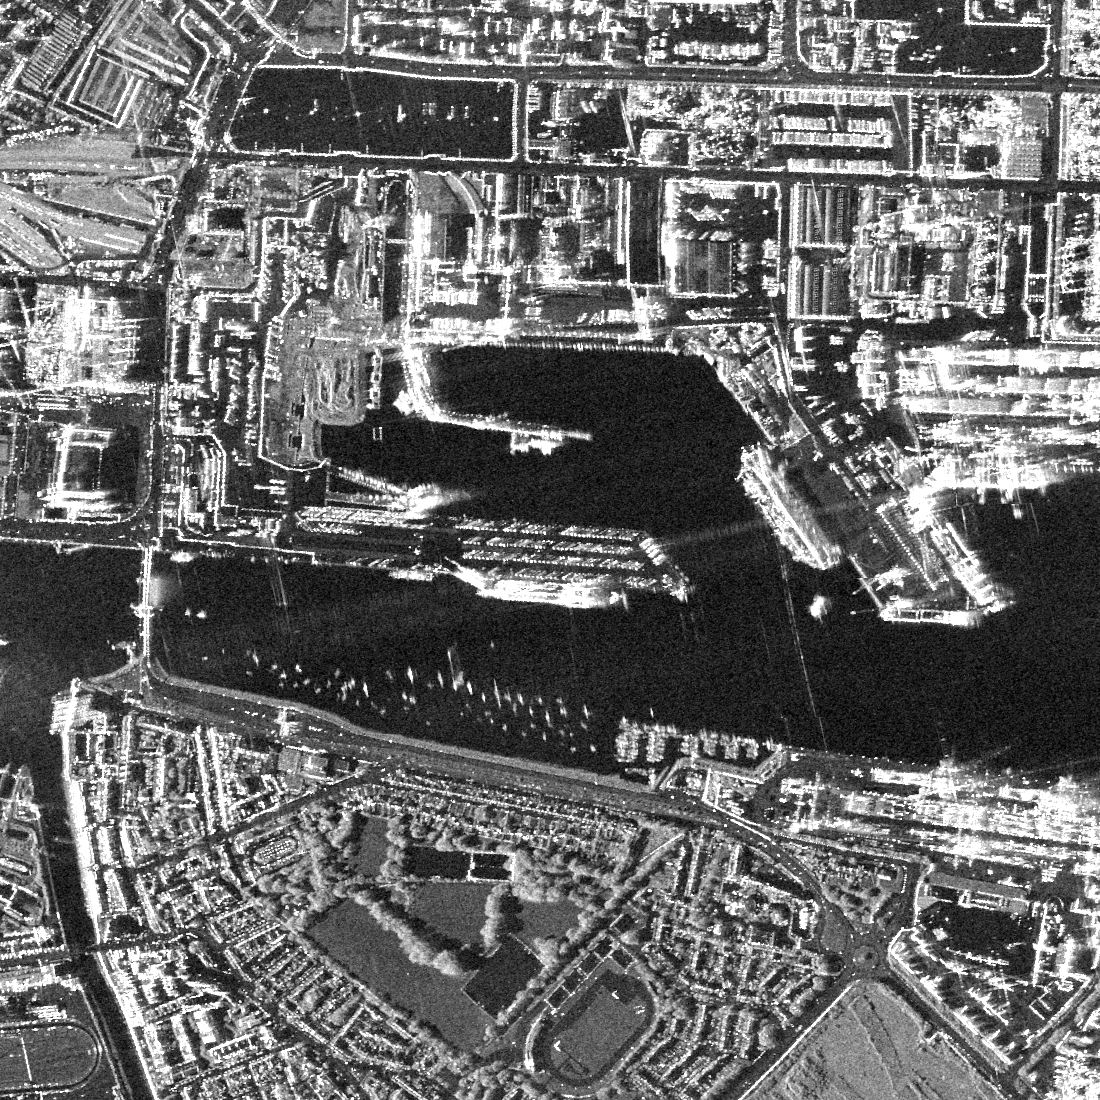
\includegraphics[width=\linewidth]{./Figures/dublin_1100_hh.png}
%DIFDELCMD <         %%%
\DIFdelendFL \DIFaddbeginFL \begin{subfigure}{0.145\textwidth}
        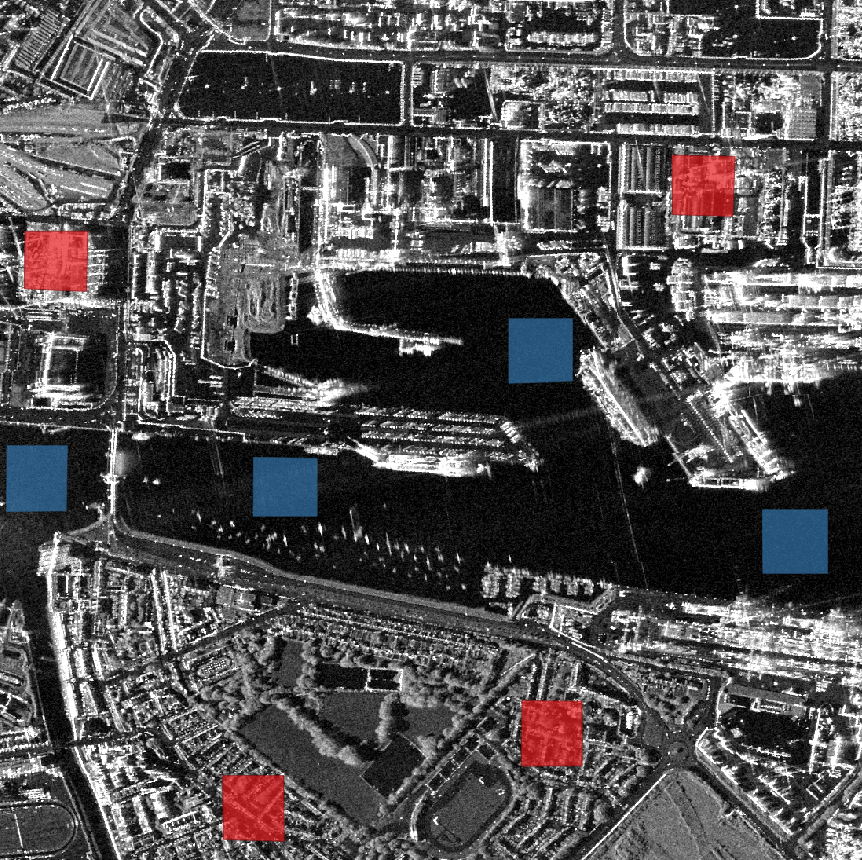
\includegraphics[width=\linewidth]{./Figures-R1/dublin_roi3.png}
        \DIFaddendFL \caption{SAR image}
        \DIFdelbeginFL %DIFDELCMD < \label{fig:dublin-a}
%DIFDELCMD <     %%%
\DIFdelendFL \DIFaddbeginFL \label{fig:dublin-sar}
    \DIFaddendFL \end{subfigure}
    \DIFdelbeginFL %DIFDELCMD < \begin{subfigure}{0.22\textwidth}
%DIFDELCMD <         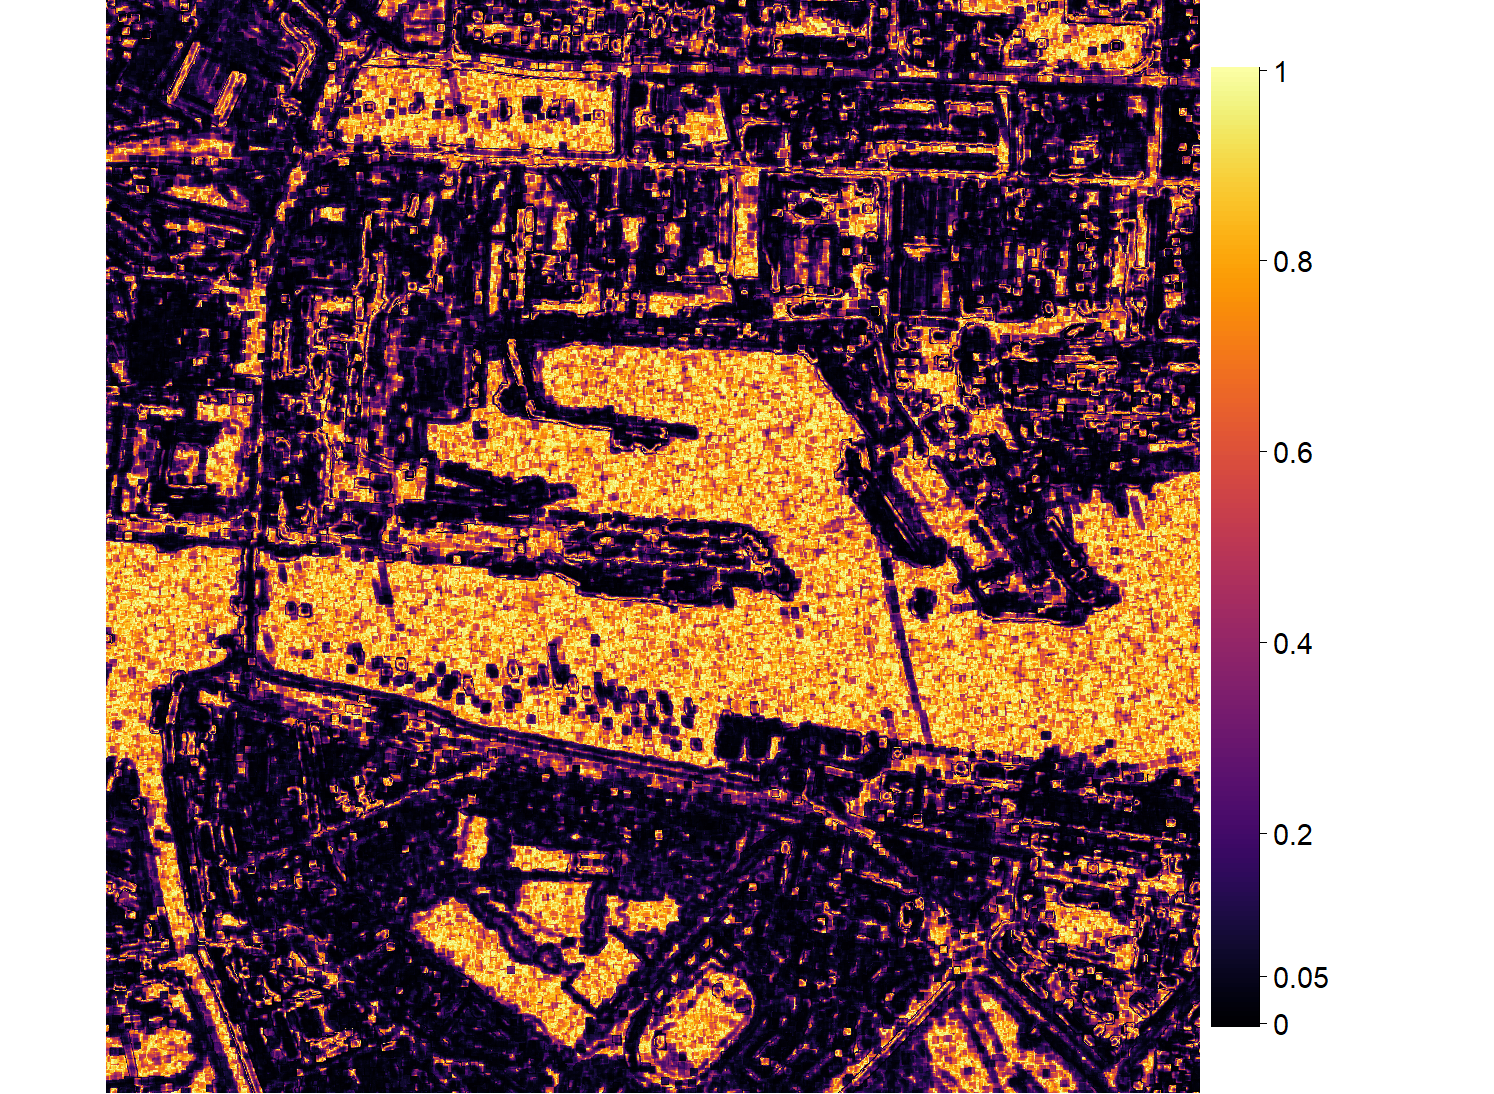
\includegraphics[width=\linewidth]{./Figures/dublin_renyi_09_w7_b100.png}
%DIFDELCMD <         %%%
\DIFdelendFL \DIFaddbeginFL \DIFaddFL{\hspace{0.00001\textwidth}
}\begin{subfigure}{0.145\textwidth}
        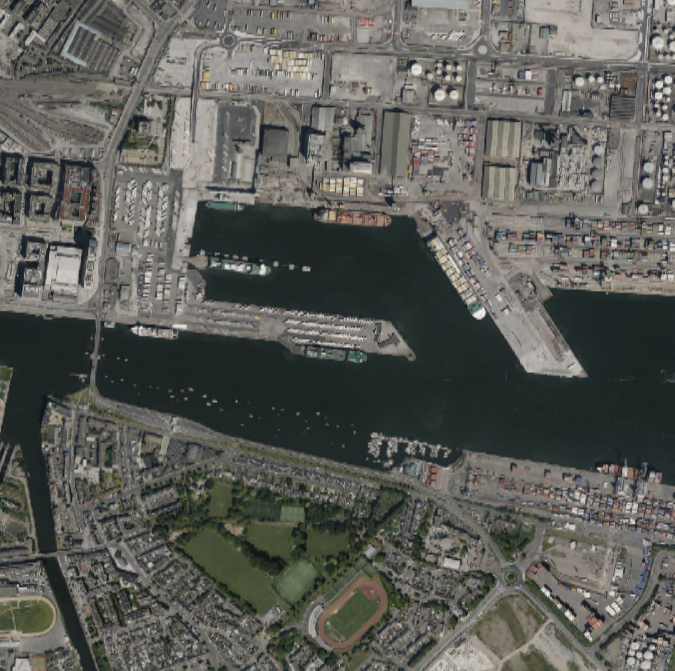
\includegraphics[width=\linewidth]{./Figures-R1/dublin.png}
        \DIFaddendFL \caption{\DIFaddbeginFL \DIFaddFL{Optical image}}
        \label{fig:dublin-optical}
    \end{subfigure}
    \DIFaddFL{\hspace{0.00001\textwidth}
    }\begin{subfigure}{0.178\textwidth}
        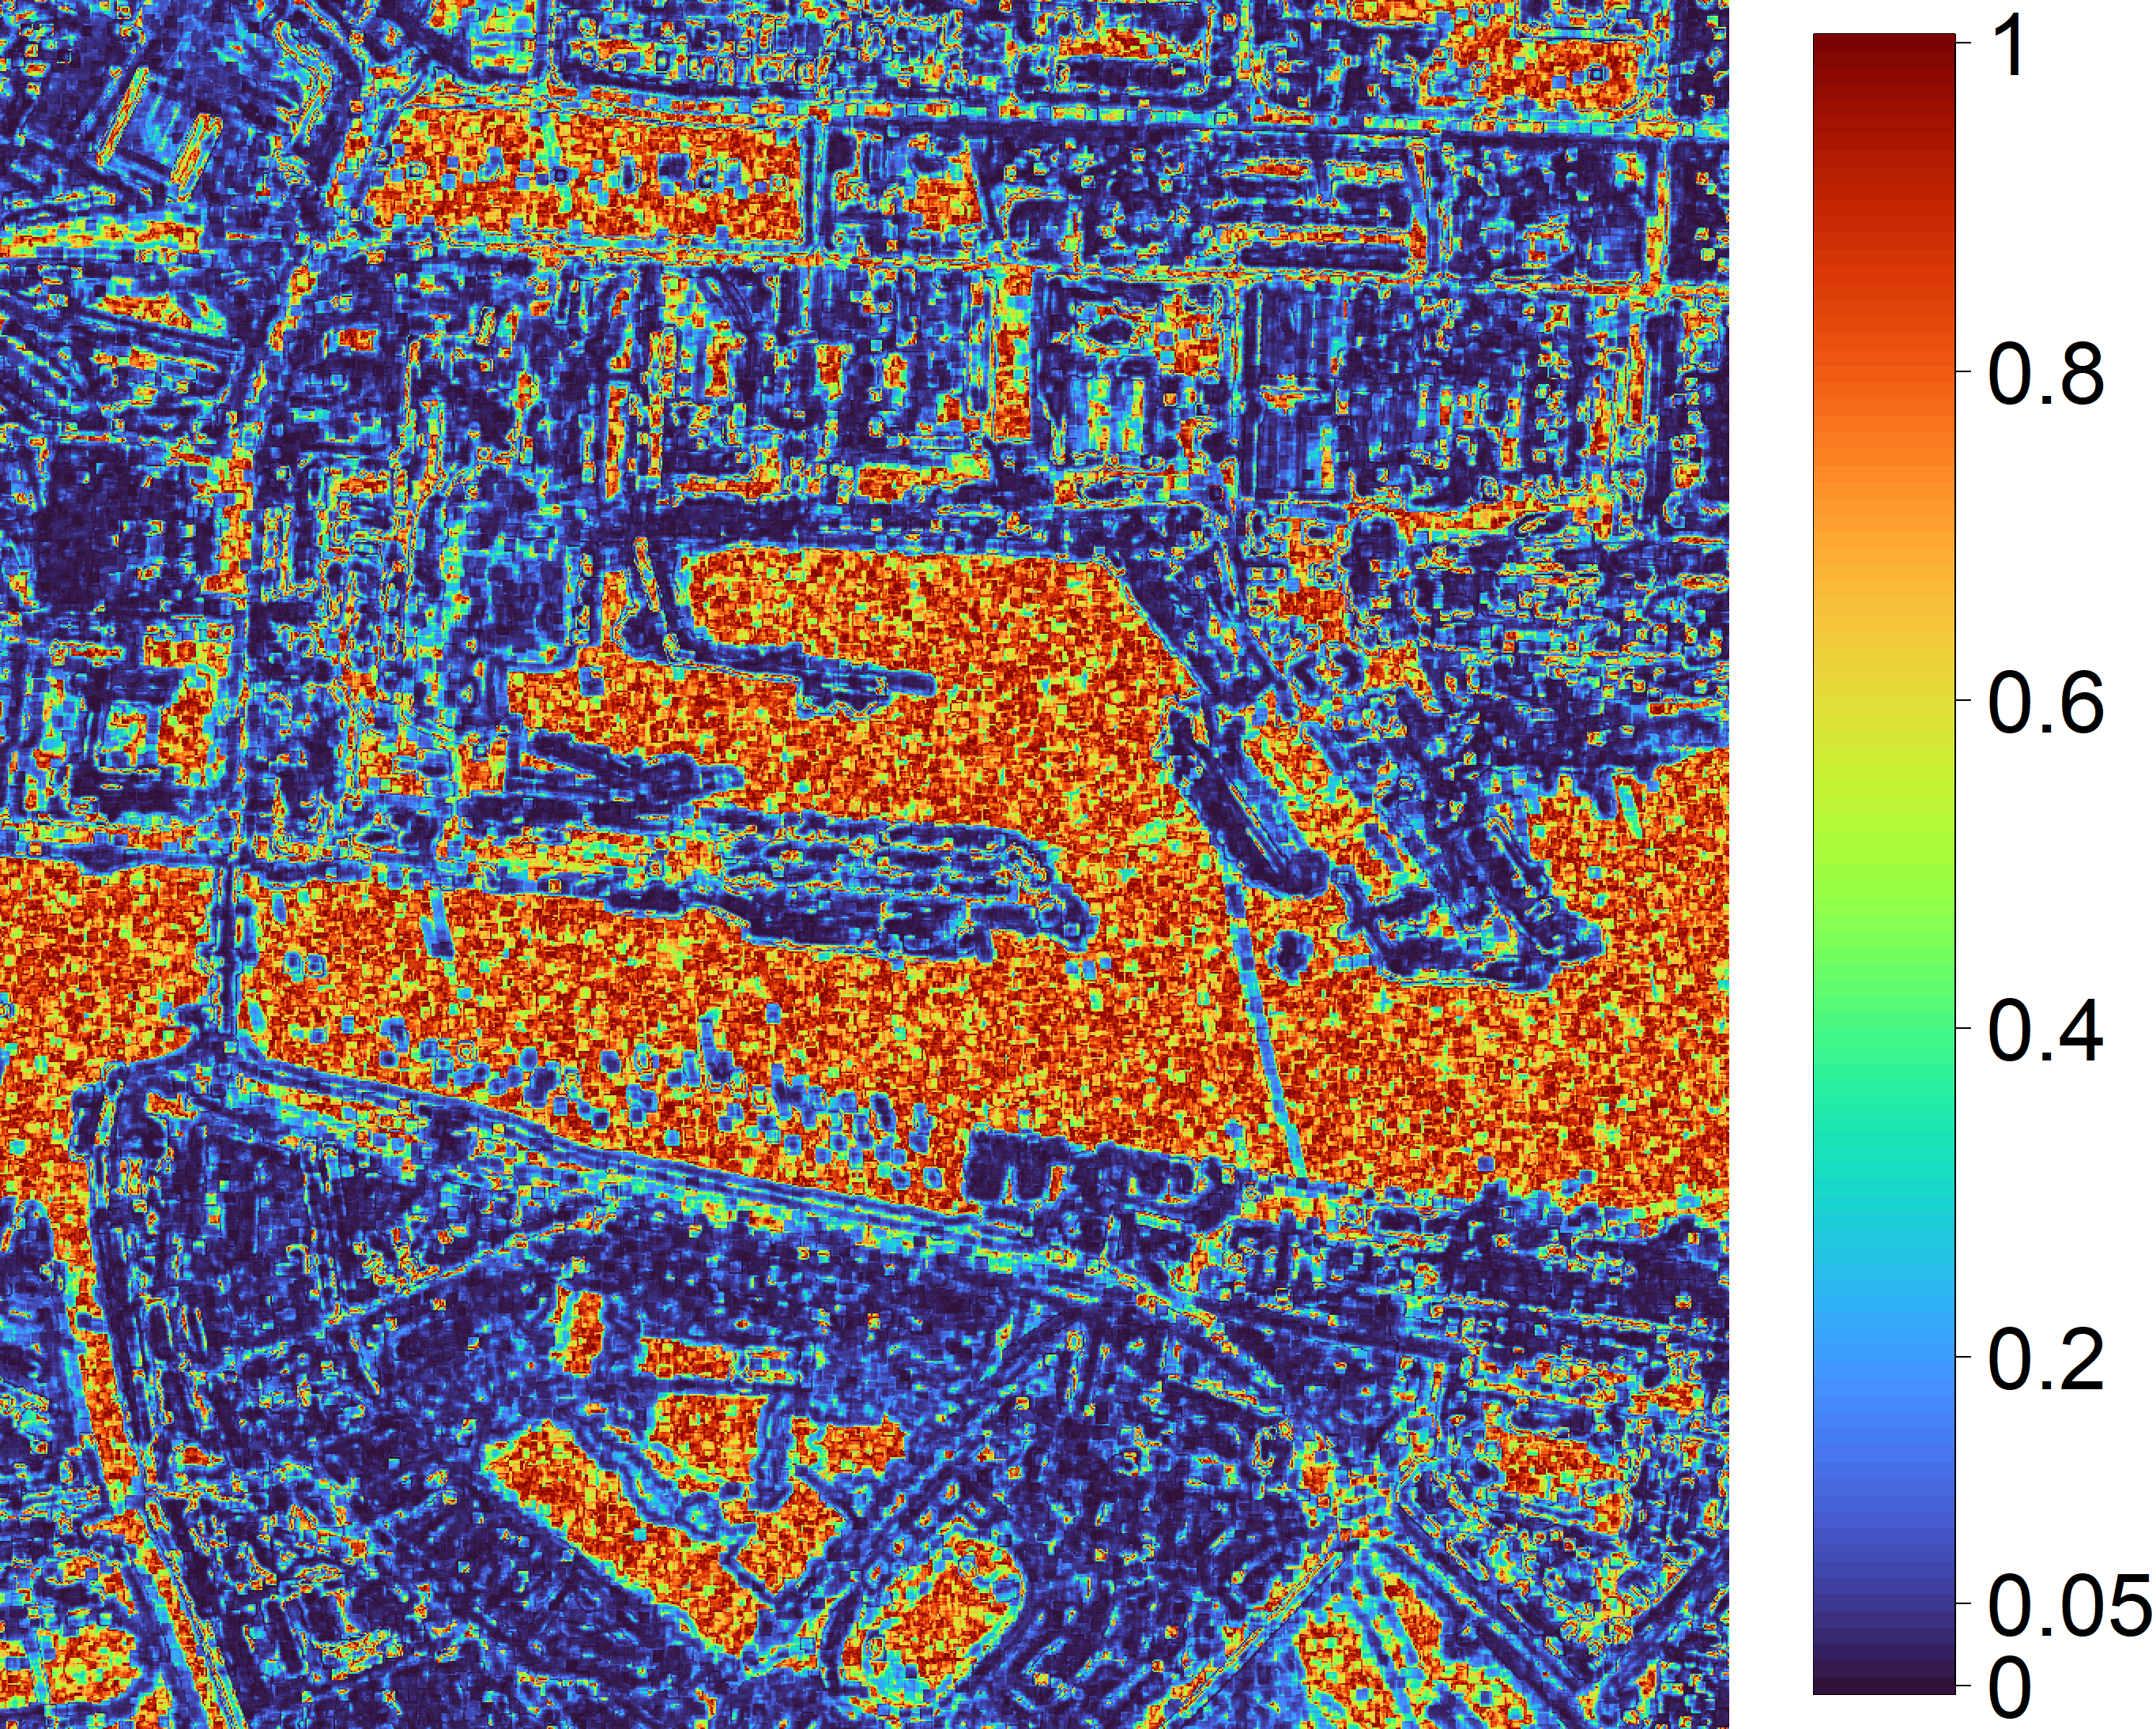
\includegraphics[width=\linewidth]{./Figures-R1/p-values_renyi-dublin-H1.png}
        \caption{\DIFaddendFL $p$-value map \DIFdelbeginFL \DIFdelFL{for }\DIFdelendFL $\small{S_{\widetilde{H}_{\lambda}}}$}
        \DIFdelbeginFL %DIFDELCMD < \label{fig:dublin-b}
%DIFDELCMD <     %%%
\DIFdelendFL \DIFaddbeginFL \label{fig:dublin-renyi}
    \DIFaddendFL \end{subfigure}
    \DIFdelbeginFL %DIFDELCMD < \begin{subfigure}{0.16\textwidth}
%DIFDELCMD <         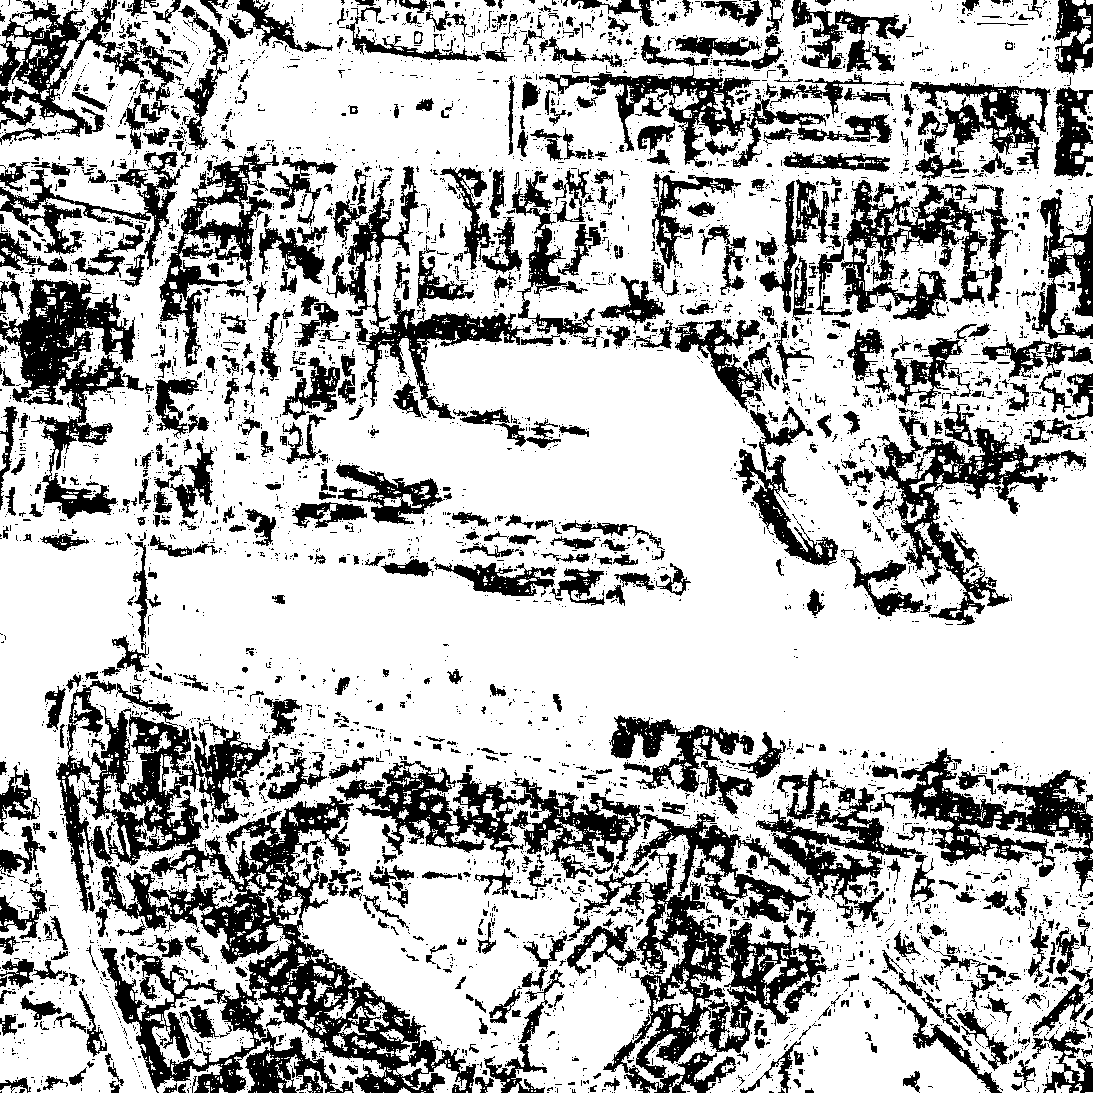
\includegraphics[width=\linewidth]{./Figures/H_005_dublin_renyi_09_w7_b100.png}
%DIFDELCMD <         %%%
\DIFdelendFL \DIFaddbeginFL \DIFaddFL{\hspace{0.00001\textwidth}
    }\begin{subfigure}{0.144\textwidth}
        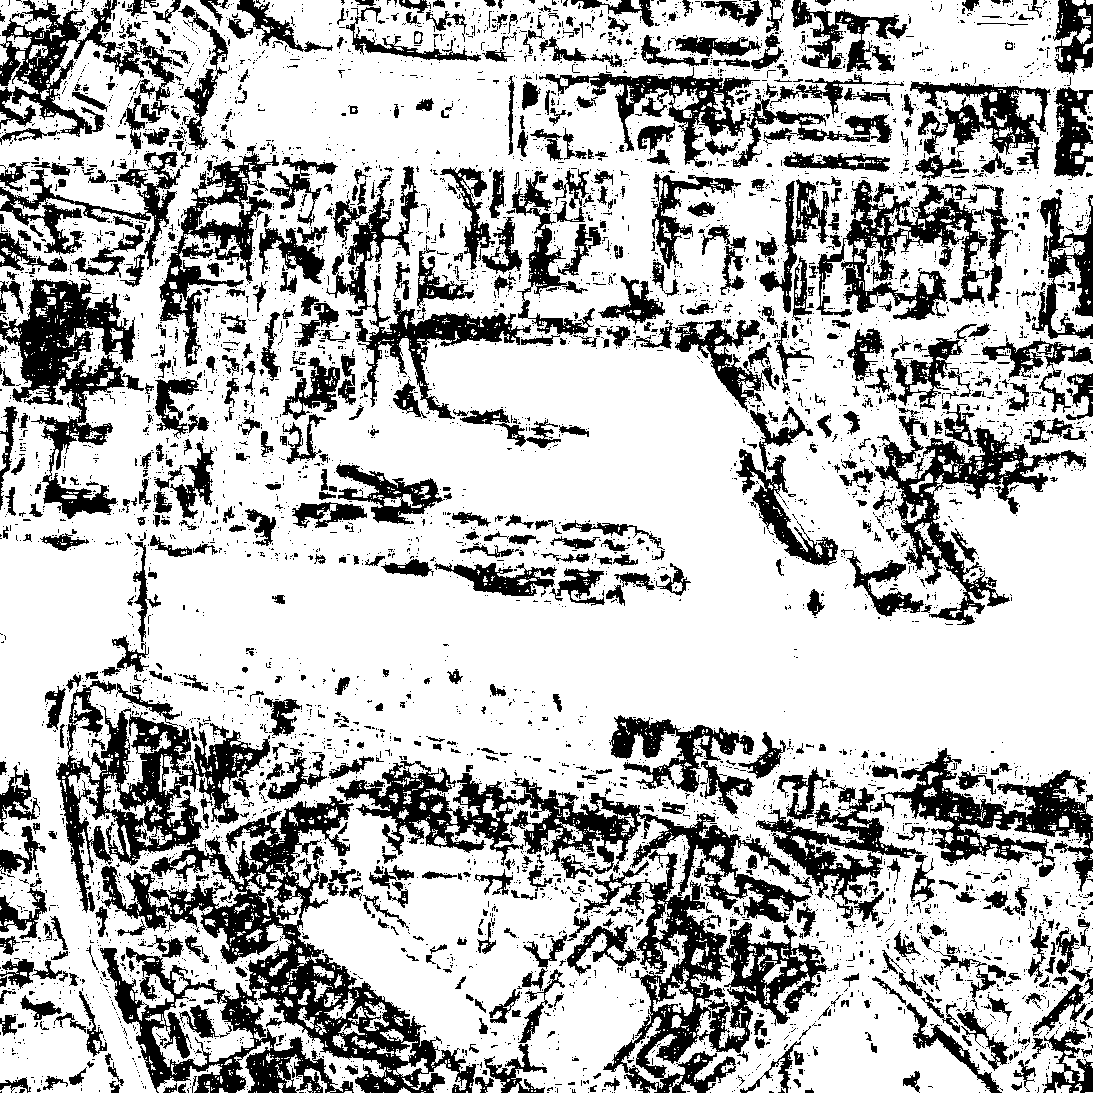
\includegraphics[width=\linewidth]{./Figures-R1/H_005_dublin_renyi.png}
        \DIFaddendFL \caption{Binary map \DIFdelbeginFL \DIFdelFL{for }\DIFdelendFL $\small{S_{\widetilde{H}_{\lambda}}}$}
        \DIFdelbeginFL %DIFDELCMD < \label{fig:dublin-c}
%DIFDELCMD <     %%%
\DIFdelendFL \DIFaddbeginFL \label{fig:dublin-005-renyi}
    \DIFaddendFL \end{subfigure}
    \DIFdelbeginFL %DIFDELCMD < \begin{subfigure}{0.22\textwidth}
%DIFDELCMD <         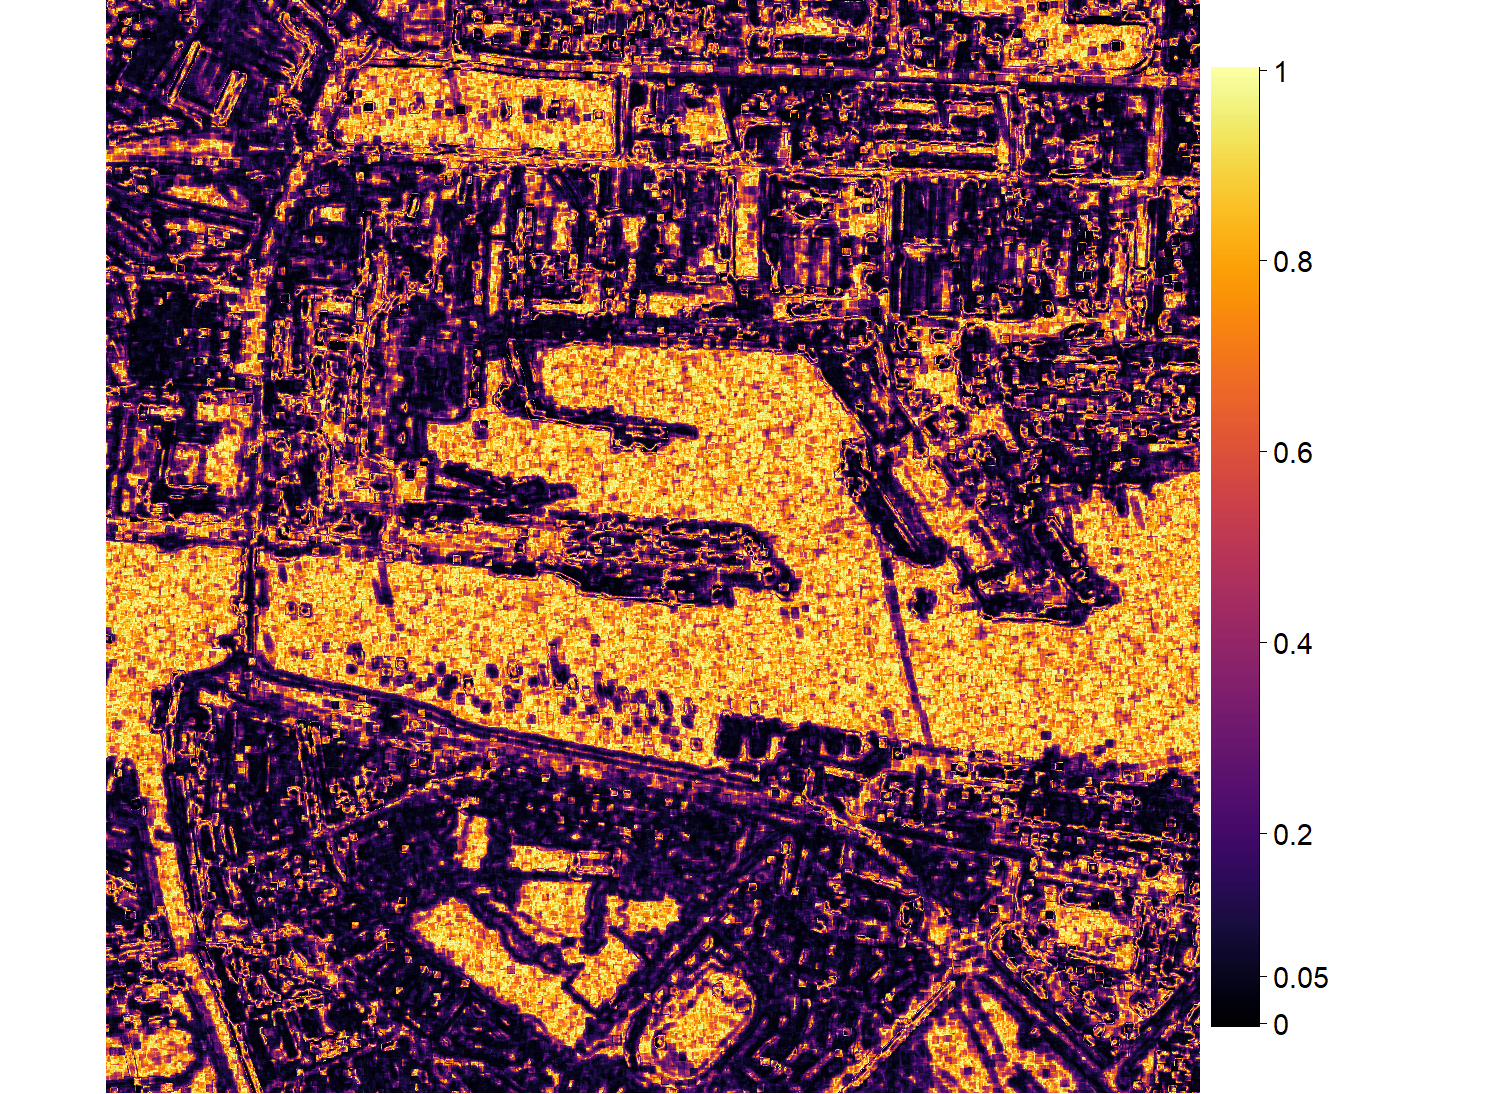
\includegraphics[width=\linewidth]{./Figures/AO_w7_L16_b100.png}
%DIFDELCMD <         %%%
\DIFdelendFL \DIFaddbeginFL \DIFaddFL{\hspace{0.00001\textwidth}
    }\begin{subfigure}{0.178\textwidth}
        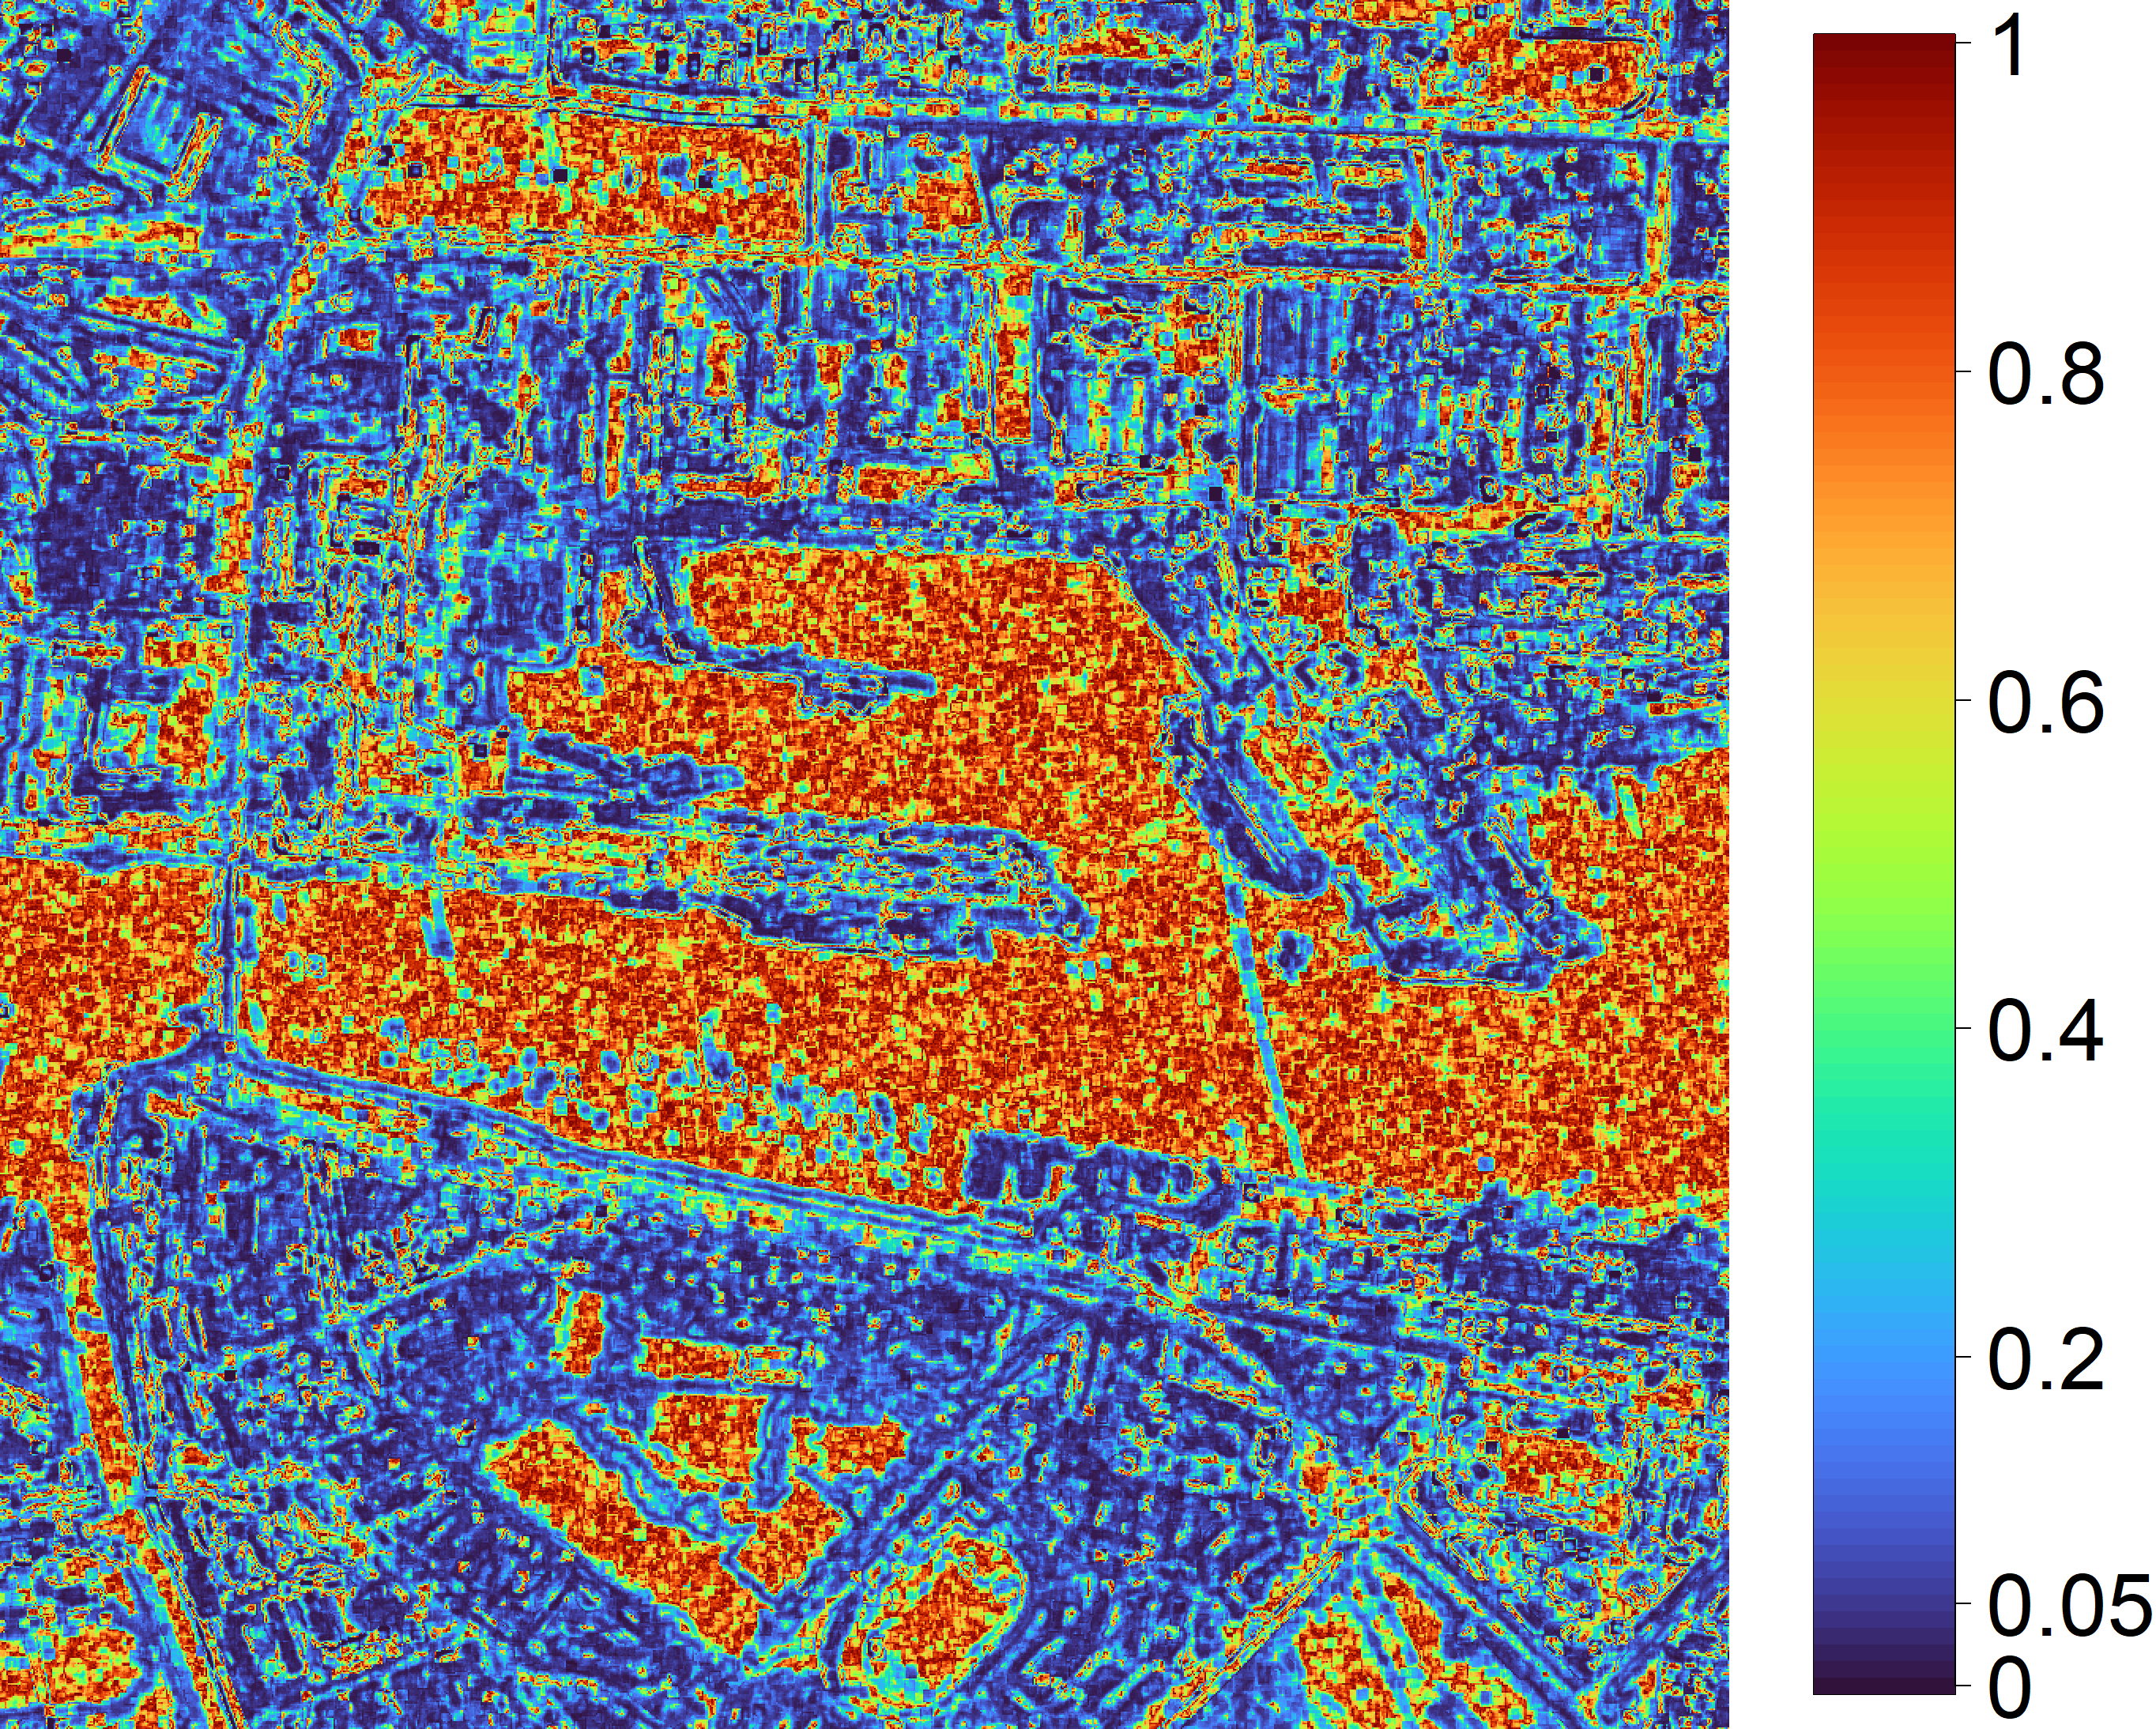
\includegraphics[width=\linewidth]{./Figures-R1/p-values_shannon-dublin-H1.png}
        \DIFaddendFL \caption{$p$-value \DIFdelbeginFL \DIFdelFL{map for $S_{\widetilde{H}_{\text{AO}}}$}%DIFDELCMD < \MBLOCKRIGHTBRACE
%DIFDELCMD <         \label{fig:dublin-d}
%DIFDELCMD <     \end{subfigure}
%DIFDELCMD <     \begin{subfigure}{0.16\textwidth}
%DIFDELCMD <         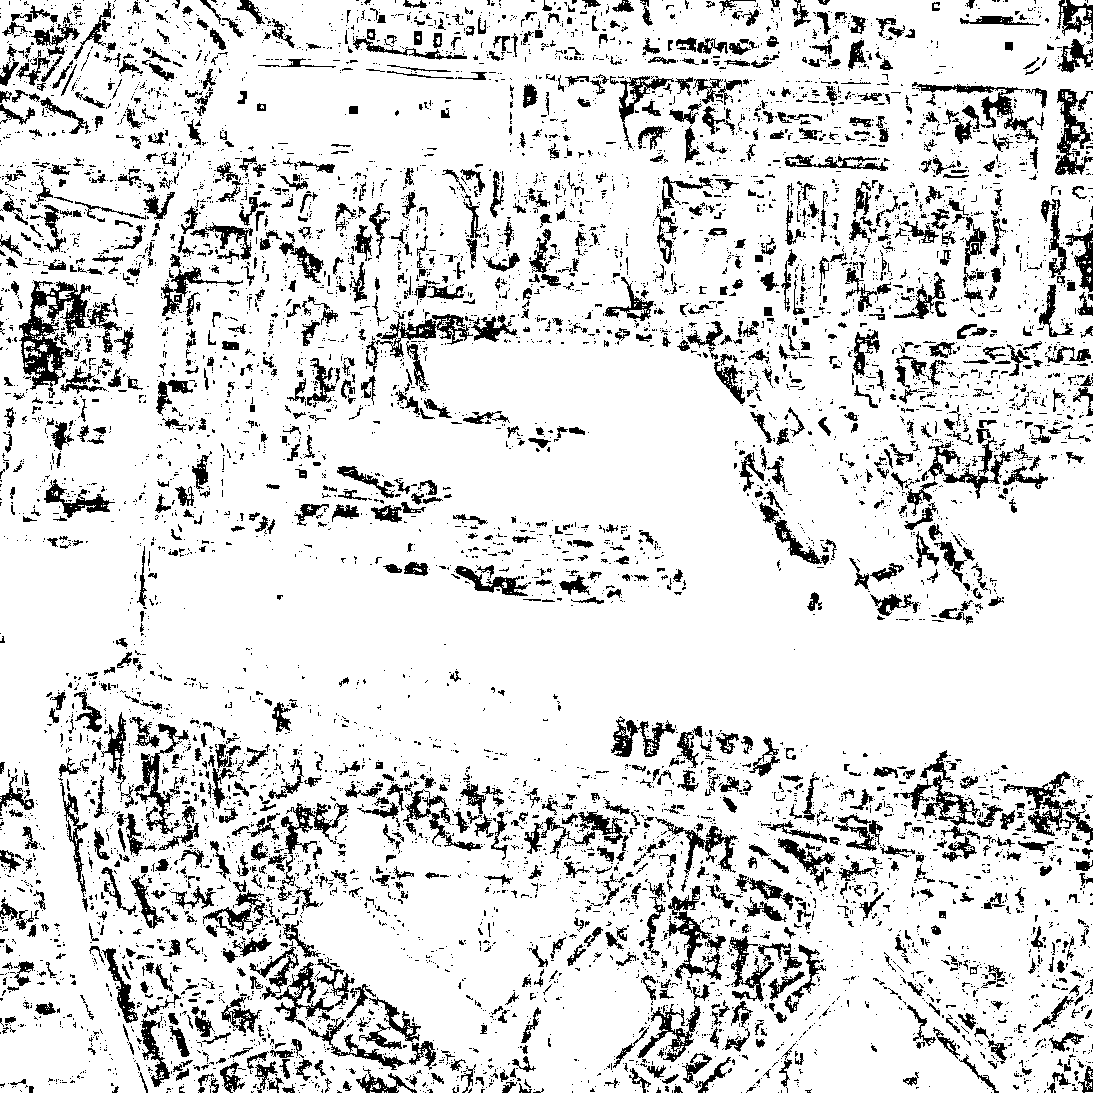
\includegraphics[width=\linewidth]{./Figures/H_005_AO_w7_L16_b100.png}
%DIFDELCMD <         \caption{%%%
\DIFdelFL{Binary map for }\DIFdelendFL $\small{S_{\widetilde{H}_{\text{AO}}}}$}
        \DIFdelbeginFL %DIFDELCMD < \label{fig:dublin-e}
%DIFDELCMD <     %%%
\DIFdelendFL \DIFaddbeginFL \label{fig:dublin-shann}
    \DIFaddendFL \end{subfigure}
    \DIFaddbeginFL \DIFaddFL{\hspace{0.0000001\textwidth}
    }\begin{subfigure}{0.144\textwidth}
        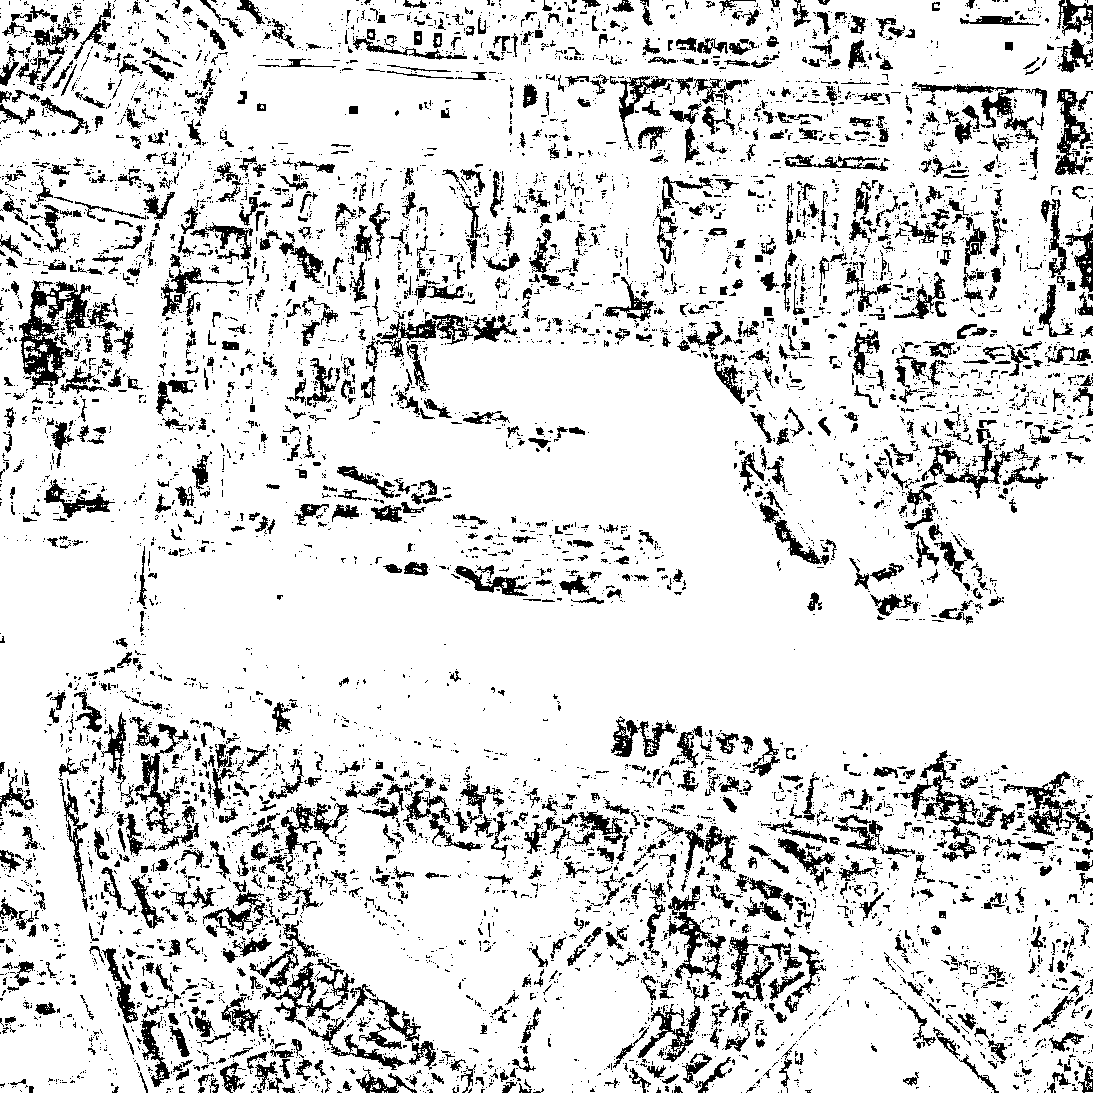
\includegraphics[width=\linewidth]{./Figures-R1/H_005_dublin-shannon.png}
        \caption{\DIFaddFL{Binary $\small{S_{\widetilde{H}_{\text{AO}}}}$}}
        \label{fig:dublin-005-shann}
    \end{subfigure}
    \DIFaddendFL \caption{Detection of heterogeneous areas in a SAR image over Dublin Port, Ireland: comparison with the tests $\small{S_{\widetilde{H}_{\lambda}}}$ and $\small{S_{\widetilde{H}_{\text{AO}}}}$.}
    \DIFdelbeginFL %DIFDELCMD < 

%DIFDELCMD <     %%%
\DIFdelendFL \label{fig:dublin}
\end{figure*}

\DIFaddbegin \subsection{\DIFadd{Quantitative Evaluation}}\label{quantitative-evaluation}

\DIFadd{Eight polygonal regions of interest (ROIs) were manually selected for
each scene (Figs.~\ref{fig:london-sar}-\ref{fig:dublin-sar}):
heterogeneous areas (red, class 1) and homogeneous areas (blue, class
0). These ROIs were rasterized to match the SAR resolution, forming a
partial ground truth. We thresholded the \(p\)-value maps at 0.05,
labeling each pixel as heterogeneous (1) or homogeneous (0) and then
compared these decision maps with the ground truth to compute: F1-score
(\(F_1\)), Kappa coefficient (\(\kappa\)), and overall accuracy (OA).
Table~\ref{tab:table_metrics} summarizes the results. Across all scenes,
the Rényi-based test outperformed Shannon's in all metrics, with notable
gains in London (\(F_1\): 0.695 vs.~0.617; \(\kappa\): 0.626 vs.~0.542),
highlighting its ability to capture heterogeneity under strong speckle
(single-look).
}

\renewcommand{\arraystretch}{1.1}

\begin{table}[hbt]
\centering\centering
\caption{\label{tab:table_metrics}\DIFaddFL{Quantitative measures of heterogeneity detection}}
\resizebox{\ifdim\width>\linewidth\linewidth\else\width\fi}{!}{
\fontsize{7}{9}\selectfont
\begin{tabu} to \linewidth {>{\centering}X>{\centering}X>{\centering}X>{\centering}X>{\centering}X}
\toprule
\multicolumn{1}{c}{\textbf{Scene}} & \multicolumn{1}{c}{\textbf{Test}} & \multicolumn{1}{c}{$\bm{F_1}$} & \multicolumn{1}{c}{$\kappa$} & \multicolumn{1}{c}{\textbf{OA}}\\
\midrule
 & $S_{\widetilde{H}_{\lambda}}$ & \bm{$0.695$} & \bm{$0.626$} & \bm{$0.877$}\\

\multirow[b]{-2}{*}{\centering\arraybackslash London} & $S_{\widetilde{H}_{\text{AO}}}$ & $0.617$ & $0.542$ & $0.854$\\
\cmidrule{1-5}
 & $S_{\widetilde{H}_{\lambda}}$ & \bm{$0.924$} & \bm{$0.861$} & \bm{$0.931$}\\

\multirow[b]{-2}{*}{\centering\arraybackslash Munich} & $S_{\widetilde{H}_{\text{AO}}}$ & $0.883$ & $0.794$ & $0.897$\\
\cmidrule{1-5}
 & $S_{\widetilde{H}_{\lambda}}$ & \bm{$0.865$} & \bm{$0.753$} & \bm{$0.875$}\\

\multirow[b]{-2}{*}{\centering\arraybackslash Dublin} & $S_{\widetilde{H}_{\text{AO}}}$ & $0.645$ & $0.464$ & $0.858$\\
\bottomrule
\end{tabu}}
\end{table}

\DIFadd{Using the same ROIs as ground truth, we evaluated the continuous
\(p\)-value maps by computing receiver operating characteristic (ROC)
curves over all decision thresholds~(Fig.~\ref{fig:roc}). Each curve
plots the probability of detection (Pd) versus the probability of false
alarm (PFA). Pd reflects the proportion of heterogeneous pixels
correctly detected, while PFA represents the proportion of homogeneous
pixels misclassified as heterogeneous.
}

\begin{figure}[hbt]
  \centering
  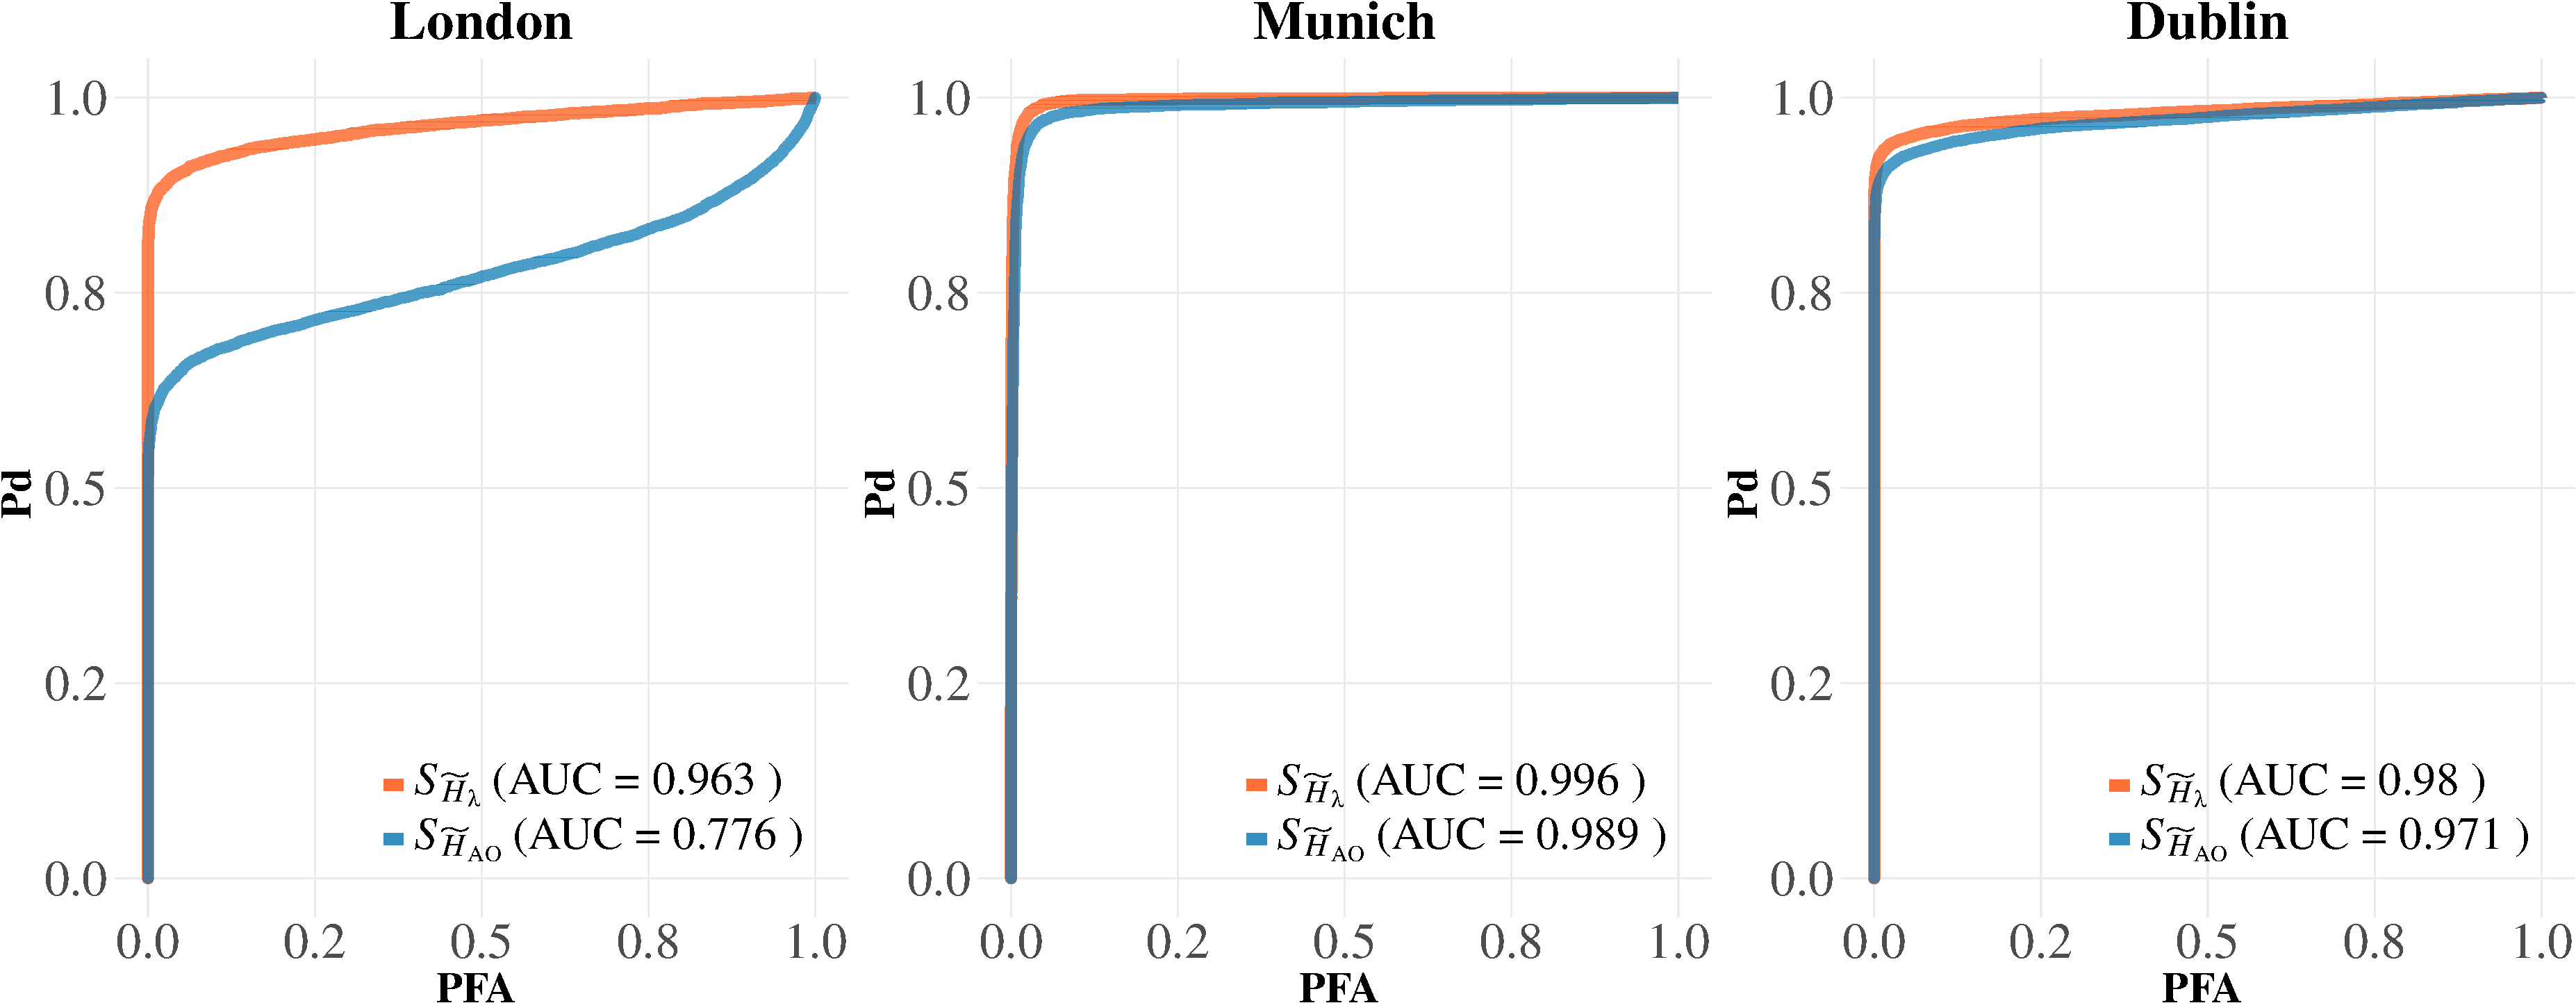
\includegraphics[width=0.49\textwidth]{Figures-R1/ROC1-1.pdf}
  \caption{\DIFaddFL{ROC curves comparing the tests $S_{\widetilde{H}_{\lambda}}$ and $S_{\widetilde{H}_{\text{AO}}}$.}}
  \label{fig:roc}
\end{figure}

\DIFadd{The area under each ROC curve (AUC) quantifies global detection
performance. The Rényi-based test achieved higher AUCs across all
scenes---London: 0.963 vs.~0.776; Munich: 0.996 vs.~0.989; Dublin: 0.980
vs.~0.971---demonstrating superior robustness compared to the
Shannon-based test under various terrain conditions and textures.
}

\DIFaddend \section{Conclusions}\label{sec:conclusion}

This study presented a \DIFdelbegin \DIFdel{new }\DIFdelend statistical approach based on Rényi entropy for
detecting heterogeneity in SAR images, distinguishing between fully
developed speckle and heterogeneous clutter. The proposed test \DIFdelbegin \DIFdel{performance was
evaluated by }\DIFdelend \DIFaddbegin \DIFadd{was
validated with synthetic experiments via }\DIFaddend a Monte Carlo study\DIFdelbegin \DIFdel{. The results showed
that the method }\DIFdelend \DIFaddbegin \DIFadd{,
demonstrating that it }\DIFaddend effectively controls the probability of Type~I
error while maintaining \DIFdelbegin \DIFdel{a }\DIFdelend high detection performance that improves \DIFdelbegin \DIFdel{as the
sample sizeincreases}\DIFdelend \DIFaddbegin \DIFadd{with
sample size}\DIFaddend .

\DIFdelbegin \DIFdel{The effectiveness of the Rényi entropy-based test in SAR images was
compared with the Shannon entropy-based test using }\DIFdelend \DIFaddbegin \DIFadd{Using SAR data, we compared the Rényi-based test with a Shannon-based
counterpart through }\DIFaddend \(p\)-value \DIFdelbegin \DIFdel{and
binary maps. The differences between the two methods are evident in the
binary maps at a \(0.05\) significance level. Although both tests
successfully detected heterogeneous regions, the }\DIFdelend \DIFaddbegin \DIFadd{maps and binary decisions. Visual
analysis showed greater sensitivity of the }\DIFaddend Rényi-based test \DIFdelbegin \DIFdel{performed better due to its flexibility in adjusting the \(\lambda\)
parameter, allowing for finer texture variation differentiation}\DIFdelend \DIFaddbegin \DIFadd{to textural
variations. Quantitative evaluation with ground truth ROIs and standard
classification metrics confirmed the superior performance of the
Rényi-based test across all scenes.
}

\DIFadd{Although machine learning-based SAR classifiers are widely used, our
focus is on interpretable, statistically grounded methods that yield
analytical significance measures. This makes them suitable for rapid
detection, screening, and environments with limited data availability}\DIFaddend .

Future work will explore \DIFdelbegin \DIFdel{additional statistical metrics to improve the comparison between both tests and better quantify their differences in
detecting heterogeneity.
}%DIFDELCMD < 

%DIFDELCMD < \appendix[Derivation of the Rényi Entropy of $\mathcal{G}^0_I$]{}
%DIFDELCMD < 

%DIFDELCMD < %%%
\DIFdel{Let \(Z \sim \mathcal{G}^0_I(\alpha, \gamma, L)\) as defined in
Ref.~\mbox{%DIFAUXCMD
\citeproc{ref-Frery2024}{{[}13{]}}}\hskip0pt%DIFAUXCMD
. We compute
\(I = \int_0^\infty [f_{\mathcal{G}^0_I}(z)]^\lambda dz\) using the pdf}%DIFDELCMD < \\
%DIFDELCMD < %%%
\begin{displaymath}
\DIFdel{f_{\mathcal{G}^0_I}(z) = C \frac{z^{L-1}}{(\gamma + Lz)^{L-\alpha}},  
\quad C = \frac{L^L \Gamma(L - \alpha)}{\gamma^\alpha \Gamma(-\alpha) \Gamma(L)}. \label{eq:pdf_G0I}
}\end{displaymath}%DIFAUXCMD
%DIFDELCMD <  %%%
\DIFdel{Setting \(t = Lz/\gamma\), we obtain}%DIFDELCMD < \\
%DIFDELCMD < %%%
\begin{displaymath}
\DIFdel{I = C^\lambda \frac{\gamma^{1-\lambda+\lambda\alpha}}{L^{\lambda L + 1 - \lambda}}  
\int_0^\infty \frac{t^{\lambda(L-1)}}{(1+t)^{\lambda(L-\alpha)}} dt.
}\end{displaymath}%DIFAUXCMD
%DIFDELCMD <  %%%
\DIFdel{Applying the Beta function identity,
\(B(a,b) = \int_0^\infty \frac{t^{a-1}}{(1+t)^{a+b}} dt\) with
\(a = \lambda(L-1) + 1\), \(b = \lambda(-\alpha+1) - 1\), we get}%DIFDELCMD < \\
%DIFDELCMD < %%%
\begin{displaymath}
\DIFdel{I= \gamma^{\,1 - \lambda}\,
   L^{\,\lambda - 1}
   \Bigl(\tfrac{\Gamma(L - \alpha)}{\Gamma(-\alpha)\,\Gamma(L)}\Bigr)^\lambda
   \,B(a,b).
}\end{displaymath}%DIFAUXCMD
%DIFDELCMD <  %%%
\DIFdel{Using the }\DIFdelend \DIFaddbegin \DIFadd{the integration of the improved }\DIFaddend Rényi \DIFdelbegin \DIFdel{entropy definition in
\eqref{E:entropy2}: \(H_\lambda(Z) = (1-\lambda)^{-1} \ln I\), and
substituting \(\gamma = -\mu(\alpha + 1)\),
we obtain the final
expression for \(\mathcal{G}^0_I(\mu, \alpha, L)\) in \eqref{eq-HGI0}}\DIFdelend \DIFaddbegin \DIFadd{estimator
into SAR classification pipelines, both supervised and unsupervised,
extending its utility beyond heterogeneity testing}\DIFaddend .

\DIFdelbegin \section*{\DIFdel{Computational Information}}%DIFAUXCMD
%DIFDELCMD < \label{computational-information}
%DIFDELCMD < %%%
\addcontentsline{toc}{section}{\DIFdel{Computational Information}}
%DIFAUXCMD
%DIFDELCMD < 

%DIFDELCMD < %%%
\DIFdel{This article was written in Quarto and is fully reproducible. We used
RStudio version 2024.12.1+563, and R version 4.4.2.
}%DIFDELCMD < 

%DIFDELCMD < %%%
\DIFdelend \section*{References}\label{references}
\addcontentsline{toc}{section}{References}

\phantomsection\label{refs}
\begin{CSLReferences}{0}{0}
\DIFdelbegin \bibitem[\citeproctext]{ref-Yu2023}
\DIFdelend \DIFaddbegin \bibitem[\citeproctext]{ref-Mondini2021}
\DIFaddend \CSLLeftMargin{{[}1{]} }%
\DIFdelbegin %DIFDELCMD < \CSLRightInline{H. Yu, X. Yin, Z. Liu, S. Zhou, C. Li, and H. Jiang,
%DIFDELCMD < {``\href{https://doi.org/10.1109/jstars.2023.3257548}{A novel
%DIFDELCMD < unsupervised evaluation metric based on heterogeneity features for SAR
%DIFDELCMD < image segmentation},''} \emph{IEEE Journal of Selected Topics in Applied
%DIFDELCMD < Earth Observations and Remote Sensing}, vol. 16, pp. 2851--2867, 2023. }
%DIFDELCMD < %%%
\DIFdelend \DIFaddbegin \CSLRightInline{A. C. Mondini, F. Guzzetti, K.-T. Chang, O. Monserrat,
T. R. Martha, and A. Manconi,
{``\href{https://doi.org/10.1016/j.earscirev.2021.103574}{Landslide
failures detection and mapping using synthetic aperture radar: Past,
present and future},''} \emph{Earth-Science Reviews}, vol. 216, p.
103574, 2021. }
\DIFaddend 

\DIFdelbegin \bibitem[\citeproctext]{ref-Akbarizadeh2012}
\DIFdelend \DIFaddbegin \bibitem[\citeproctext]{ref-Zeng2020}
\DIFaddend \CSLLeftMargin{{[}2{]} }%
\DIFdelbegin %DIFDELCMD < \CSLRightInline{G. Akbarizadeh,
%DIFDELCMD < {``\href{https://doi.org/10.1109/tgrs.2012.2194787}{A new
%DIFDELCMD < statistical-based kurtosis wavelet energy feature for texture
%DIFDELCMD < recognition of SAR images},''} \emph{IEEE Transactions on Geoscience and
%DIFDELCMD < Remote Sensing}, vol. 50, no. 11, pp. 4358--4368, 2012. }
%DIFDELCMD < %%%
\DIFdelend \DIFaddbegin \CSLRightInline{Z. Zeng \emph{et al.},
{``\href{https://doi.org/10.1016/j.jhydrol.2019.124377}{Towards high
resolution flood monitoring: An integrated methodology using passive
microwave brightness temperatures and sentinel synthetic aperture radar
imagery},''} \emph{Journal of Hydrology}, vol. 582, p. 124377, 2020. }
\DIFaddend 

\DIFdelbegin \bibitem[\citeproctext]{ref-Mondini2021}
\DIFdelend \DIFaddbegin \bibitem[\citeproctext]{ref-Baraha2023}
\DIFaddend \CSLLeftMargin{{[}3{]} }%
\DIFdelbegin %DIFDELCMD < \CSLRightInline{A. C. Mondini, F. Guzzetti, K.-T. Chang, O. Monserrat,
%DIFDELCMD < T. R. Martha, and A. Manconi,
%DIFDELCMD < {``\href{https://doi.org/10.1016/j.earscirev.2021.103574}{Landslide
%DIFDELCMD < failures detection and mapping using synthetic aperture radar: Past,
%DIFDELCMD < present and future},''} \emph{Earth-Science Reviews}, vol. 216, p.
%DIFDELCMD < 103574, 2021. }
%DIFDELCMD < %%%
\DIFdelend \DIFaddbegin \CSLRightInline{S. Baraha and A. K. Sahoo,
{``\href{https://doi.org/10.1016/j.sigpro.2023.109156}{Synthetic
aperture radar image and its despeckling using variational methods: A
review of recent trends},''} \emph{Signal Processing}, vol. 212, p.
109156, 2023. }
\DIFaddend 

\DIFdelbegin \bibitem[\citeproctext]{ref-Zeng2020}
\DIFdelend \DIFaddbegin \bibitem[\citeproctext]{ref-Nascimento2014}
\DIFaddend \CSLLeftMargin{{[}4{]} }%
\DIFdelbegin %DIFDELCMD < \CSLRightInline{Z. Zeng \emph{et al.},
%DIFDELCMD < {``\href{https://doi.org/10.1016/j.jhydrol.2019.124377}{Towards high
%DIFDELCMD < resolution flood monitoring: An integrated methodology using passive
%DIFDELCMD < microwave brightness temperatures and sentinel synthetic aperture radar
%DIFDELCMD < imagery},''} \emph{Journal of Hydrology}, vol. 582, p. 124377, 2020. }
%DIFDELCMD < %%%
\DIFdelend \DIFaddbegin \CSLRightInline{A. D. C. Nascimento, M. M. Horta, A. C. Frery, and R. J.
Cintra, {``Comparing edge detection methods based on stochastic
entropies and distances for {PolSAR} imagery,''} \emph{{IEEE} Journal of
Selected Topics in Applied Earth Observations and Remote Sensing}, vol.
7, no. 2, pp. 648--663, 2014. }
\DIFaddend 

\DIFdelbegin \bibitem[\citeproctext]{ref-Argenti2013}
\DIFdelend \DIFaddbegin \bibitem[\citeproctext]{ref-Nobre2016}
\DIFaddend \CSLLeftMargin{{[}5{]} }%
\DIFdelbegin %DIFDELCMD < \CSLRightInline{F. Argenti, A. Lapini, T. Bianchi, and L. Alparone,
%DIFDELCMD < {``\href{https://doi.org/10.1109/mgrs.2013.2277512}{A tutorial on
%DIFDELCMD < speckle reduction in synthetic aperture radar images},''} \emph{IEEE
%DIFDELCMD < Geoscience and Remote Sensing Magazine}, vol. 1, no. 3, pp. 6--35, 2013.
%DIFDELCMD < }
%DIFDELCMD < %%%
\DIFdelend \DIFaddbegin \CSLRightInline{R. H. Nobre, F. A. A. Rodrigues, R. C. P. Marques, J. S.
Nobre, J. F. S. R. Neto, and F. N. S. Medeiros,
{``\href{https://doi.org/10.1109/lsp.2016.2606760}{SAR image
segmentation with {R}ényi's entropy},''} \emph{IEEE Signal Processing
Letters}, vol. 23, no. 11, pp. 1551--1555, 2016. }
\DIFaddend 

\DIFdelbegin \bibitem[\citeproctext]{ref-Choi2019}
\DIFdelend \DIFaddbegin \bibitem[\citeproctext]{ref-Chan2022}
\DIFaddend \CSLLeftMargin{{[}6{]} }%
\DIFdelbegin %DIFDELCMD < \CSLRightInline{H. Choi and J. Jeong,
%DIFDELCMD < {``\href{https://doi.org/10.3390/rs11101184}{Speckle noise reduction
%DIFDELCMD < technique for SAR images using statistical characteristics of speckle
%DIFDELCMD < noise and discrete wavelet transform},''} \emph{Remote Sensing}, vol.
%DIFDELCMD < 11, no. 10, p. 1184, 2019. }
%DIFDELCMD < %%%
\DIFdelend \DIFaddbegin \CSLRightInline{D. Chan, J. Gambini, and A. C. Frery,
{``\href{https://doi.org/10.3390/rs14030509}{Entropy-based non-local
means filter for single-look SAR speckle reduction},''} \emph{Remote
Sensing}, vol. 14, no. 3, p. 509, 2022. }
\DIFaddend 

\DIFdelbegin \bibitem[\citeproctext]{ref-Baraha2023}
\DIFdelend \DIFaddbegin \bibitem[\citeproctext]{ref-Shannon1948}
\DIFaddend \CSLLeftMargin{{[}7{]} }%
\DIFdelbegin %DIFDELCMD < \CSLRightInline{S. Baraha and A. K. Sahoo,
%DIFDELCMD < {``\href{https://doi.org/10.1016/j.sigpro.2023.109156}{Synthetic
%DIFDELCMD < aperture radar image and its despeckling using variational methods: A
%DIFDELCMD < review of recent trends},''} \emph{Signal Processing}, vol. 212, p.
%DIFDELCMD < 109156, 2023. }
%DIFDELCMD < %%%
\DIFdelend \DIFaddbegin \CSLRightInline{C. E. Shannon, {``A mathematical theory of
communication,''} \emph{The Bell System Technical Journal}, vol. 27, no.
3, pp. 379--423, 1948. }
\DIFaddend 

\DIFdelbegin \bibitem[\citeproctext]{ref-Nascimento2014}
\DIFdelend \DIFaddbegin \bibitem[\citeproctext]{ref-Cassetti2022}
\DIFaddend \CSLLeftMargin{{[}8{]} }%
\DIFdelbegin %DIFDELCMD < \CSLRightInline{A. D. C. Nascimento, M. M. Horta, A. C. Frery, and R. J.
%DIFDELCMD < Cintra, {``Comparing edge detection methods based on stochastic
%DIFDELCMD < entropies and distances for {PolSAR} imagery,''} \emph{{IEEE} Journal of
%DIFDELCMD < Selected Topics in Applied Earth Observations and Remote Sensing}, vol.
%DIFDELCMD < 7, no. 2, pp. 648--663, 2014. }
%DIFDELCMD < %%%
\DIFdelend \DIFaddbegin \CSLRightInline{J. Cassetti, D. Delgadino, A. Rey, and A. C. Frery,
{``Entropy estimators in {SAR} image classification,''} \emph{Entropy},
vol. 24, no. 4, p. 509, 2022. }
\DIFaddend 

\DIFdelbegin \bibitem[\citeproctext]{ref-Nobre2016}
\DIFdelend \DIFaddbegin \bibitem[\citeproctext]{ref-Gallet2024}
\DIFaddend \CSLLeftMargin{{[}9{]} }%
\DIFdelbegin %DIFDELCMD < \CSLRightInline{R. H. Nobre, F. A. A. Rodrigues, R. C. P. Marques, J. S.
%DIFDELCMD < Nobre, J. F. S. R. Neto, and F. N. S. Medeiros,
%DIFDELCMD < {``\href{https://doi.org/10.1109/lsp.2016.2606760}{SAR image
%DIFDELCMD < segmentation with {R}ényi's entropy},''} \emph{IEEE Signal Processing
%DIFDELCMD < Letters}, vol. 23, no. 11, pp. 1551--1555, 2016. }
%DIFDELCMD < %%%
\DIFdelend \DIFaddbegin \CSLRightInline{M. Gallet, A. Mian, and A. Atto,
{``\href{https://doi.org/10.1109/icassp48485.2024.10448227}{Renyi
divergences learning for explainable classification of {SAR} image
pairs},''} in \emph{2024 {IEEE} {I}nternational {C}onference on
{A}coustics, {S}peech and {S}ignal {P}rocessing {(ICASSP)}}, 2024, pp.
7445--7449. }
\DIFaddend 

\DIFdelbegin \bibitem[\citeproctext]{ref-Cassetti2022}
\DIFdelend \DIFaddbegin \bibitem[\citeproctext]{ref-Parikh2019}
\DIFaddend \CSLLeftMargin{{[}10{]} }%
\DIFdelbegin %DIFDELCMD < \CSLRightInline{J. Cassetti, D. Delgadino, A. Rey, and A. C. Frery,
%DIFDELCMD < {``Entropy estimators in {SAR} image classification,''} \emph{Entropy},
%DIFDELCMD < vol. 24, no. 4, p. 509, 2022. }
%DIFDELCMD < %%%
\DIFdelend \DIFaddbegin \CSLRightInline{H. Parikh, S. Patel, and V. Patel,
{``\href{https://doi.org/10.1080/19479832.2019.1655489}{Classification
of {SAR} and {PolSAR} images using deep learning: A review},''}
\emph{International Journal of Image and Data Fusion}, vol. 11, no. 1,
pp. 1--32, 2019. }
\DIFaddend 

\DIFdelbegin \bibitem[\citeproctext]{ref-Chan2022}
\DIFdelend \DIFaddbegin \bibitem[\citeproctext]{ref-Frery2024}
\DIFaddend \CSLLeftMargin{{[}11{]} }%
\DIFdelbegin %DIFDELCMD < \CSLRightInline{D. Chan, J. Gambini, and A. C. Frery,
%DIFDELCMD < {``\href{https://doi.org/10.3390/rs14030509}{Entropy-based non-local
%DIFDELCMD < means filter for single-look SAR speckle reduction},''} \emph{Remote
%DIFDELCMD < Sensing}, vol. 14, no. 3, p. 509, 2022. }
%DIFDELCMD < %%%
\DIFdelend \DIFaddbegin \CSLRightInline{A. C. Frery, J. Alpala, and A. D. C. Nascimento,
{``\href{https://doi.org/10.3390/rs16111973}{Identifying heterogeneity
in {SAR} data with new test statistics},''} \emph{Remote Sensing}, vol.
16, no. 11, p. 1973, 2024. }
\DIFaddend 

\DIFdelbegin \bibitem[\citeproctext]{ref-Shannon1948}
\DIFdelend \DIFaddbegin \bibitem[\citeproctext]{ref-Frery1997}
\DIFaddend \CSLLeftMargin{{[}12{]} }%
\DIFdelbegin %DIFDELCMD < \CSLRightInline{C. E. Shannon, {``A mathematical theory of
%DIFDELCMD < communication,''} \emph{The Bell System Technical Journal}, vol. 27, no.
%DIFDELCMD < 3, pp. 379--423, 1948. }
%DIFDELCMD < %%%
\DIFdelend \DIFaddbegin \CSLRightInline{A. C. Frery, H.-J. Muller, C. C. F. Yanasse, and S. J.
S. SantAnna, {``A model for extremely heterogeneous clutter,''}
\emph{{IEEE} Transactions on Geoscience and Remote Sensing}, vol. 35,
no. 3, pp. 648--659, 1997. }
\DIFaddend 

\DIFdelbegin \bibitem[\citeproctext]{ref-Frery2024}
\DIFdelend \DIFaddbegin \bibitem[\citeproctext]{ref-AlLabadi2024}
\DIFaddend \CSLLeftMargin{{[}13{]} }%
\DIFdelbegin %DIFDELCMD < \CSLRightInline{A. C. Frery, J. Alpala, and A. D. C. Nascimento,
%DIFDELCMD < {``\href{https://doi.org/10.3390/rs16111973}{Identifying heterogeneity
%DIFDELCMD < in {SAR} data with new test statistics},''} \emph{Remote Sensing}, vol.
%DIFDELCMD < 16, no. 11, p. 1973, 2024. }
%DIFDELCMD < %%%
\DIFdelend \DIFaddbegin \CSLRightInline{L. Al-Labadi, Z. Chu, and Y. Xu,
{``\href{https://doi.org/10.1007/s00180-024-01507-z}{Advancements in
{R}ényi entropy and divergence estimation for model assessment},''}
\emph{Computational Statistics}, 2024. }
\DIFaddend 

\DIFdelbegin \bibitem[\citeproctext]{ref-Frery1997}
\DIFdelend \DIFaddbegin \bibitem[\citeproctext]{ref-Alpala2024}
\DIFaddend \CSLLeftMargin{{[}14{]} }%
\DIFdelbegin %DIFDELCMD < \CSLRightInline{A. C. Frery, H.-J. Muller, C. C. F. Yanasse, and S. J.
%DIFDELCMD < S. SantAnna, {``A model for extremely heterogeneous clutter,''}
%DIFDELCMD < \emph{{IEEE} Transactions on Geoscience and Remote Sensing}, vol. 35,
%DIFDELCMD < no. 3, pp. 648--659, 1997. }
%DIFDELCMD < %%%
\DIFdelend \DIFaddbegin \CSLRightInline{R. J. Alpala, A. D. C. Nascimento, and A. C. Frery,
{``\href{https://doi.org/10.1109/migars61408.2024.10544448}{Identifying
departures from the fully developed speckle hypothesis in intensity
{SAR} data with non-parametric estimation of the entropy},''} in
\emph{2024 {I}nternational {C}onference on {M}achine {I}ntelligence for
{G}eo{A}nalytics and {R}emote {S}ensing ({MIGARS})}, 2024, pp. 1--4. }
\DIFaddend 

\DIFdelbegin \bibitem[\citeproctext]{ref-renyi1961measures}
\DIFdelend \DIFaddbegin \bibitem[\citeproctext]{ref-vasicek1976test}
\DIFaddend \CSLLeftMargin{{[}15{]} }%
\DIFdelbegin %DIFDELCMD < \CSLRightInline{A. Rényi, {``On measures of entropy and information,''}
%DIFDELCMD < in \emph{Proceedings of the fourth {B}erkeley {S}ymposium on
%DIFDELCMD < {M}athematical {S}tatistics and {P}robability}, 1961, vol. 4, pp.
%DIFDELCMD < 547--562. }
%DIFDELCMD < 

%DIFDELCMD < \bibitem[\citeproctext]{ref-Ribeiro2021}
%DIFDELCMD < \CSLLeftMargin{{[}16{]} }%%%
%DIF < 
%DIFDELCMD < \CSLRightInline{M. Ribeiro \emph{et al.},
%DIFDELCMD < {``\href{https://doi.org/10.3390/e23020222}{The entropy universe},''}
%DIFDELCMD < \emph{Entropy}, vol. 23, no. 2, p. 222, 2021. }
%DIFDELCMD < 

%DIFDELCMD < \bibitem[\citeproctext]{ref-vasicek1976test}
%DIFDELCMD < \CSLLeftMargin{{[}17{]} }%%%
%DIF < 
\DIFdelend \CSLRightInline{O. Vasicek, {``A test for normality based on sample
entropy,''} \emph{Journal of the Royal Statistical Society Series B:
Statistical Methodology}, vol. 38, no. 1, pp. 54--59, 1976. }

\DIFdelbegin \bibitem[\citeproctext]{ref-Bert1992}
%DIFDELCMD < \CSLLeftMargin{{[}18{]} }%%%
%DIF < 
%DIFDELCMD < \CSLRightInline{B. Van Es, {``Estimating functionals related to a
%DIFDELCMD < density by a class of statistics based on spacings,''}
%DIFDELCMD < \emph{Scandinavian Journal of Statistics}, vol. 19, pp. 61--72, 1992. }
%DIFDELCMD < 

%DIFDELCMD < \bibitem[\citeproctext]{ref-Ebrahimi1994}
%DIFDELCMD < \CSLLeftMargin{{[}19{]} }%%%
%DIF < 
%DIFDELCMD < \CSLRightInline{N. Ebrahimi, K. Pflughoeft, and E. S. Soofi, {``Two
%DIFDELCMD < measures of sample entropy,''} \emph{Statistics \& Probability Letters},
%DIFDELCMD < vol. 20, no. 3, pp. 225--234, 1994. }
%DIFDELCMD < 

%DIFDELCMD < \bibitem[\citeproctext]{ref-Wieczorkowski1999}
%DIFDELCMD < \CSLLeftMargin{{[}20{]} }%%%
%DIF < 
%DIFDELCMD < \CSLRightInline{R. Wieczorkowski and P. Grzegorzewski, {``Entropy
%DIFDELCMD < estimators-improvements and comparisons,''} \emph{Communications in
%DIFDELCMD < Statistics-Simulation and Computation}, vol. 28, no. 2, pp. 541--567,
%DIFDELCMD < 1999. }
%DIFDELCMD < 

%DIFDELCMD < %%%
\DIFdelend \bibitem[\citeproctext]{ref-IbrahimAlOmari2014}
\DIFdelbegin %DIFDELCMD < \CSLLeftMargin{{[}21{]} }%%%
\DIFdelend \DIFaddbegin \CSLLeftMargin{{[}16{]} }\DIFaddend %
\CSLRightInline{A. I. Al-Omari, {``Estimation of entropy using random
sampling,''} \emph{Journal of Computational and Applied Mathematics},
vol. 261, pp. 95--102, 2014. }
\DIFdelbegin %DIFDELCMD < 

%DIFDELCMD < \bibitem[\citeproctext]{ref-AlLabadi2024}
%DIFDELCMD < \CSLLeftMargin{{[}22{]} }%%%
%DIF < 
%DIFDELCMD < \CSLRightInline{L. Al-Labadi, Z. Chu, and Y. Xu,
%DIFDELCMD < {``\href{https://doi.org/10.1007/s00180-024-01507-z}{Advancements in
%DIFDELCMD < {R}ényi entropy and divergence estimation for model assessment},''}
%DIFDELCMD < \emph{Computational Statistics}, 2024. }
%DIFDELCMD < 

%DIFDELCMD < \bibitem[\citeproctext]{ref-Alpala2024}
%DIFDELCMD < \CSLLeftMargin{{[}23{]} }%%%
%DIF < 
%DIFDELCMD < \CSLRightInline{R. J. Alpala, A. D. C. Nascimento, and A. C. Frery,
%DIFDELCMD < {``\href{https://doi.org/10.1109/migars61408.2024.10544448}{Identifying
%DIFDELCMD < departures from the fully developed speckle hypothesis in intensity
%DIFDELCMD < {SAR} data with non-parametric estimation of the entropy},''} in
%DIFDELCMD < \emph{2024 {I}nternational {C}onference on {M}achine {I}ntelligence for
%DIFDELCMD < {G}eo{A}nalytics and {R}emote {S}ensing ({MIGARS})}, 2024, pp. 1--4. }
%DIFDELCMD < %%%
\DIFdelend 

\end{CSLReferences}


% Can use something like this to put references on a page
% by themselves when using endfloat and the captionsoff option.
\ifCLASSOPTIONcaptionsoff
  \newpage
\fi

% trigger a \newpage just before the given reference
% number - used to balance the columns on the last page
% adjust value as needed - may need to be readjusted if
% the document is modified later
%\IEEEtriggeratref{8}
% The "triggered" command can be changed if desired:
%\IEEEtriggercmd{\enlargethispage{-5in}}

% Uncomment when use biblatex with style=ieee
%\renewcommand{\bibfont}{\footnotesize} % for IEEE bibfont size

\pagebreak[3]
% that's all folks
\end{document}

